\chapter{Syntactically driven metathesis}\label{ch:SynMet}

\section{Introduction}
In this chapter I analyse the morphological use of metathesis
in Amarasi to mark discourse structures.
The final member of a phrase or clause uses
metathesis to mark that the situation/event encoded
by the clause is unresolved and requires another clause to achieve resolution.
A discourse U\=/form (unmetathesised) typically
occurs in a parallel and complementary relationship
with an M\=/form (metathesised), the latter of which resolves the former.

Example \qf{ex:02/08/13, p.20 -2} is a question-answer
pair in which a question with a final U\=/form
is resolved by an answer in the M\=/form.
Example \qf{ex:130909-6, 0.39 -2} contains two events.
The second event is encoded in the M\=/form and is dependent
on the prior clause with a final U\=/form for its realisation.

\begin{exe}
	\ex{\glll \textnormal{\tcb{Q:}} hoo \bxA{mu-be\tbr{ʔi}}? \hspace{10mm} \textnormal{\tcb{A:}} au \bxB{u-be\tbr{iʔ}}! {\lk}\\
						{} hoo {\gp}mu-beʔi {} {} au {\gp}u-beʔi \\
						{} {\hoo} \gp\muu-capable{\tbrU} {} {} {\au} \gp\qu-capable{\tbrM} \\
			\glt	\lh{Q: }`Can you do it?' \hspace{19.75mm}`Yes I can!'
						\txrf{observation 02/08/13, p.20}}\vspace{4pt}\label{ex:02/08/13, p.20 -2} 
	\ex{\glll	m-ak hai nua =kai \bxA{m-taiko\tbr{bi}} =m hai \bxB{m-ma\tbr{et}} okeʔ {\lk}\\
						m-ak hai nua =kai {\gp}m-taikobi =ma hai {\gp}m-mate okeʔ \\
						\m-say {\hai} two {\kai} \gp\m-fall{\tbrU} =and {\hai} \gp\m-die{\tbrM} all \\
			\glt	`So we two will fall down and (then) both die.'
						\txrf{130909-6, 0.39} {\emb{130909-6-00-39.mp3}{\spk{}}{\apl}}}\label{ex:130909-6, 0.39 -2}
\end{exe}

Discourse U\=/forms are used by speakers to signal that
the event or situation is not resolved.
Such a U\=/form represents half of a whole
which requires resolution by another clause.
Discourse-driven U\=/forms leave the audience in a state of  suspense
with the speaker signalling that more information
is required to resolve the situation or event
encoded by a clause with a final U\=/form.

Nearly all word classes which are not canonical nominals
(as defined in \srf{sec:NomWorCla}) have discourse-driven U\=/forms.
These word classes are listed in \qf{ex:WorClaDisMet} below.
I refer to these word classes as \emph{non-nominals} throughout this chapter.
The label `non-nominal' is not ideal as place names,
demonstratives, and pronouns all have many nominal characteristics.
However, there does not seem to be a more appropriate term
which covers all of the word classes in \qf{ex:WorClaDisMet}.

\begin{exe}
	\ex{Word classes with discourse-driven U\=/forms:}\label{ex:WorClaDisMet}
		\begin{xlist}
			\ex{verbs}
			\ex{numerals}
			\ex{place names}
			\ex{number enclitics (\ve{eni} `{\ein}', \ve{=esa}, `{\es}')}
			\ex{demonstratives (\ve{nana} `{\naan}')}
			\ex{determiners (\ve{=ana} `{\aan}')}
			\ex{pronouns (\ve{ini} `{\iin}', \ve{sini} `{\siin}', \ve{hiti} `{\hiit}')}
			\ex{adverbials (\ve{=ena} `{\een}', \ve{=aha} `just')}
		\end{xlist}
\end{exe}

The use of U\=/forms is productive for verbs, numerals, and place names.
For the other word classes listed in \qf{ex:WorClaDisMet},
particularly the number enclitic \ve{=eni} `{\ein}',
the adverbials \ve{=ena} `{\een}' or \ve{=aha} `just',
as well as the demonstratives and determiners,
the use of U\=/forms is less productive, though there
are still many instances in which U\=/forms with
these latter classes signal a lack of resolution.

Discourse U\=/forms typically occur in certain constructions and environments.
These constructions and environments include dependent coordination (\srf{sec:DepCoo}),
tail-head linkage (\srf{sec:TaiHeaLin}), poetic parallelism (\srf{sec:PoePar}),
chiasmus (\srf{sec:CenChi}) and interactions between speakers (\srf{sec:IntUnm}).
These five constructions are summarised in \trf{tab:ConDisUfoTypOcc}
above along with the typical structure of each.
There are 423 discourse-driven U\=/forms in my corpus.
Of these, 406 (96\%) clearly occur in one of the five
constructions/environments given in \trf{tab:ConDisUfoTypOcc}.\footnote{
		With 423 attestations, discourse (un)metathesis is a
		well-attested morphological process.
		For comparison, my corpus has 152 instances of partial reduplication (\srf{sec:Red})
		and 48 of the reciprocal prefix \ve{ma(k)-} (\srf{sec:RecPre}).}

\begin{table}[ht]
	\caption[Constructions in which discourse U\=/forms typically occur]
					{Constructions in which discourse U\=/forms typically occur\su{†}}\label{tab:ConDisUfoTypOcc}
	\centering
		\begin{threeparttable}[b]
		\begin{tabular}{rll}
			\lsptoprule
			Construction & Typical Structure  &\\ \midrule
				&&\\[-6pt]
			Dependent coordination &
				\xytext{\fbox{event\sub{1}{\U}}\xybarconnect[2][->]{2}&(conj.)&\fbox{event\sub{2}({\M})}} &\S\ref{sec:DepCoo}\\
				&&\\[-6pt]\hline
				&&\\[-3pt]
			Tail-head linkage & 
				\xytext{\fbox{event\sub{1}{\M}}\xybarconnect[2][-](D,D){1}&\fbox{event\sub{1}{\U}}\xybarconnect[2][->]{2}&(conj.)&\fbox{event\sub{2}\vp{\M}}} &\S\ref{sec:TaiHeaLin}\\
				&&\\[-6pt]\hline
				&&\\[-6pt]
			Poetic parallelism &
				\xytext{\fbox{synonym\sub{1}{\U}}\xybarconnect[2][-](D,D){2}\xybarconnect[2][->]{2}&conj.&\fbox{synonym\sub{2}{\M}}} &\S\ref{sec:PoePar}\\
				&&\\[-6pt]\hline
				&&\\[-3pt]
			Chiasmus & 
				\xytext{\fbox{information\sub{1}}\xybarconnect[2][-](D,D){2}\xybarconnect[2][<-]{1}&\fbox{U\=/form\vp{\sub{1}}}\xybarconnect[2][->]{1}&\fbox{information\sub{1}}} &\S\ref{sec:CenChi}\\
				&&\\[-6pt]\hline
				&&\\[-6pt]
			Interaction & 
				\xytext{Speaker\sub{1}:&\fbox{U\=/form}\xybarconnect[2][-](D,D){2}\xybarconnect[2][->]{2}&Speaker\sub{2}:&\fbox{M\=/form}} &\S\ref{sec:IntUnm}\\
				&&\\[-6pt] %\hline
				\lspbottomrule
				\end{tabular}
			\begin{tablenotes}
				\item [†] An arrow indicates the form which resolves a U\=/form
												and a line joining two forms indicates forms
												which are semantically identical or parallel.
												Event\sub{1} and event\sub{2} refer to
												two different events or situations,
												with event\sub{1} beginning before event\sub{2}.
			\end{tablenotes}
		\end{threeparttable}
\end{table}

Before I discuss the details of U\=/forms in Amarasi discourse,
I discuss several other facts which provide helpful background information:
the co-occurrence of syntactically driven M\=/forms
and discourse-driven U\=/forms (\srf{sec:SynDisDriMet}),
the fact that the M\=/form is the semantically
unmarked form of non-nominals (\srf{sec:DefFor1}),
phonotactic constraints which block the use
of discourse U\=/forms (\srf{sec:PhoCon}),
and some of the general structures of Amarasi discourse (\srf{sec:DisStrAma}).

\section{Syntactically and discourse-driven metathesis}\label{sec:SynDisDriMet}
Discourse-driven U\=/forms occur with
the final members of phrases, while syntactically driven
M\=/forms occur with the medial members of phrases.
As a result, they are in complementary distribution and 
there is no competition between these two morphological uses of metathesis.
Two illustrative examples are given in \qf{ex2:160326, 5.37}
and \qf{ex2:160326, 18.26} below.

In \qf{ex2:160326, 5.37} the first member of the serial verb
construction \ve{ta-hiin t-ana} `figure out, get to know'
occurs in the M\=/form to mark that
it is modified by the second verb, as discussed in \srf{sec:SVC},
while the final verb occurs in the U\=/form
to signal that the entire verb phrase requires more information to achieve resolution.
See example \qf{ex:160326, 5.37-5.45} on page \pageref{ex:160326, 5.37-5.45}
for more discussion of \qf{ex2:160326, 5.37} and its context.

\begin{exe}
	\ex{\glll	siin neem na-tua Koorʔoot ees reʔ oras mee \hspace{35mm} ka= ta-hi\tbr{in} t-a\tbr{na} =f.\\
						sini neem na-tua Koorʔoto esa reʔ oras mee {} ka= ta-hini t-ana =f.\\
						{\siin} {\nema} \na-settle Koro{\Q}oto{\M} {\esc} {\req} time where {} {\ka}= {\tg}-know{\tbrM} {\tg}-{\ana\tbrU} ={\fa}\\
			\glt	`They came and settled in Koro{\Q}oto, it was at a time which hasn't been figured out.'
						\txrf{160326, 5.37} {\emb{160326-05-37.mp3}{\spk{}}{\apl}}}\label{ex2:160326, 5.37}
\end{exe}

Similarly, in \qf{ex2:160326, 18.26} below the first member
of the noun phrase \ve{kaan auk-k=eni} `praise names' occurs in the M\=/form to signal
that it is modified by the following nominal,
as discussed in Chapter \ref{ch:SynMet}.
This nominal in turn occurs in the M\=/form due to the following
vowel-initial enclitic, as discussed in Chapter \ref{ch:PhoMet}.
The final member of this phrase is the number enclitic \ve{=eni} `{\ein}'
which occurs in the U\=/form to signal that the entire phrase requires
more information to achieve resolution.
See example \qf{ex:160326, 18.26} on page \pageref{ex:160326, 18.26}
for more discussion of this example.

\begin{exe}
	\ex{\glll	siin naiʔ Bain mone \sf{kusus}, \hspace{60mm} siin ka\tbr{an} a\tbr{uk}-k=e\tbr{ni} bisa, Mea aiʔ Tutun.\\
						sini naiʔ Bani mone \sf{kusus} {} sini kana aku-k=eni bisa Mea aiʔ Tutun\\
						{\siin} {\naiq} Bani{\M} male exclusive {} {\siin} name{\tbrM} praise.name{\tbrMv}-{\k=\ein\tbrU} can Mea or Tutun\\
			\glt	`Members of the Bani clan classified as male can
						exclusively have the praise names Mea or Tutun.'
						\txrf{160326, 18.26} {\emb{160326-18-26.mp3}{\spk{}}{\apl}}}\label{ex2:160326, 18.26}
\end{exe}

To summarise, syntactically driven M\=/forms only
occur with medial members of phrases, while discourse
driven U\=/forms only occur with final members of phrases.
As a result, there is no competition between them.
In a single phrase the medial members
can occur in the M\=/form to signal the internal
syntactic structure of the phrase, while the final
member can occur in the U\=/form to signal the discourse
status of the entire phrase.
\section{The nominal word class}\label{sec:NomWorCla}
Content words (non-functors) in Amarasi fall into
two major word classes: nominals and verbs.
Some roots are specified as nominal roots,
some roots are specified as verbal roots and some 
roots are precategorial \citep{don08}, being specified as neither nominal nor verbal.
\trf{tab:AmaWorCla} lists the most salient morphosyntactic criteria
which allow us to distinguish between nominals and verbs in Amarasi.

\begin{table}[h]
	\caption[Amarasi word classes]{Amarasi word classes\su{†}}\label{tab:AmaWorCla}
	\centering
		\begin{threeparttable}\stl{0.4em}
			\begin{tabular}{rcccccccc}\lsptoprule
											&agr-&{\at}&{\b}&{\mak}&C{\#}{\ra}{\0}&\tsc{subj/obj}&=Det&=Num\\ \midrule
				Nominal 			&--&--&--&--&{✔}&{✔}&{✔}&{✔}\\
				Precategorial	&{✔}&{✔}&{✔}&{✔}&{✔}&{✔}&{✔}&{✔}\\
				Verb	 				&{✔}&{✔}&{✔}&{✔}&--&--&--&--\\ \lspbottomrule
			\end{tabular}
		\begin{tablenotes}
			\item[†]	agr-: take verbal agreement prefixes (\srf{sec:VerAgrPre}),
								{\at} can be nominalised with the circumfix \ve{a-{\ldots}-t} (\srf{sec:NomA--t}),
								{\b} can take the transitive suffix \ve{-b} (\srf{sec:TraSuf}), 
								{\mak} can take the reciprocal prefix \ve{ma(k)-} (\srf{sec:RecPre}),
								C{\#}{\ra}{\0} final consonant can be deleted to derive verbs (\srf{sec:BasVerDer}),
								\tsc{subj/obj} can be the subject or object of a verb,
								=Det can take definiteness marking determiners (\srf{sec:Det}),
								=Num can take number enclitics (\srf{sec:NumEnc sec:OthNomMod}).
		\end{tablenotes}
		\end{threeparttable}
\end{table}

In this section I discuss the four criteria in \trf{tab:AmaWorCla}
which allow us to identify a nominal word class:
verbal derivation (\srf{sec:BasVerDer}),
verbal arguments (\srf{sec:VerArg}), determiner modification (\srf{sec:Det})
and number enclitic modification (\srf{sec:NumEnc}).

There is no morphosyntactic basis for distinguishing
separate classes of nouns and adjectives.
All differences in the behaviour of these putative 
categories are straightforwardly explained by their semantics.
For instance, only adjective-like nominals have been attested modified by \ve{besi} `very'.
This can be explained by the fact that some
nominals, such as \ve{reʔuf} `bad', are gradable,
while other nominals, such as \ve{fatu} `stone', are not gradable in Amarasi.

When it is necessary to distinguish between these semantic categories,
I call nominals which refer to things \emph{thing nominals}
and nominals which describe such things \emph{property nominals}.
Many nominals do not belong clearly to either of these semantic categories.
Three such examples are: \ve{mnanuʔ} `long/length, deep/depth'
\ve{kase} `foreign(er)' and \ve{anaʔ} `small, baby'.

\subsection{Base for verbal derivation}\label{sec:BasVerDer}
Amarasi has a morphological process of subtraction which derives a verb from a nominal.
Under this process the final consonant of a nominal root is deleted.
Verbs derived by this process are usually intransitive.
Examples of verbs derived from nominals by word-final consonant deletion
are given in \qf{ex:VCNoun->VVerb} below.
Verbs are listed with the \tsc{3sg} prefix \ve{na-/n-}.

In many cases the deleted consonant is historically analysable as a suffix.
Thus, for instance, Amarasi \ve{mnasiʔ} `aged, old'
is cognate with Termanu `old' \it{lasi-k} and Dengka `old' \it{lasi-ʔ}
with a final suffix \it{-k/-ʔ} which is
a productive suffix in the languages of Rote.
However, such final consonants are no longer
analysable as suffixes in Amarasi.

Furthermore, such nominal/verb pairs include several
in which the final consonant of the noun is an inheritance from Proto-Malayo-Polynesian.
Examples include are *quza\tbr{n} > \ve{ura\tbr{n}} `rain' {\ra} \ve{na-ʔura} `rains',
*ma-diŋdi\tbr{ŋ} > \ve{mainiki\tbr{n}} `cold' {\ra} \ve{n-mainiki} `is cold',
and *tapi\tbr{s} > \ve{tai\tbr{s}} `sarong' {\ra} \ve{na-tai} `clothes s.o.'.

\begin{exe}
	\ex{{\ldots}VC{\#} nominal {\ra} {\ldots}V{\#} verb}\label{ex:VCNoun->VVerb}
		\sn{\stl{0.4em}\gw\begin{tabular}{llcll}
			`rain'					&\ve{ura\tbr{n}} 			&\ra& \ve{na-ʔura} 		& `rains'\\
			`cold' 					&\ve{mainiki\tbr{n}}	&\ra& \ve{n-mainiki}	& `is cold' \\
			`sea snail' 		&\ve{kbatu\tbr{s}}		&\ra& \ve{na-kbatu} 	& `gathers sea snails' \\
			`digging stick'	&\ve{ʔsua\tbr{k}}			&\ra& \ve{na-ʔsua} 		& `digs with a digging stick' \\
			`umbrella' 			&\ve{tenu\tbr{k}}			&\ra& \ve{n-tenu} 		& `shades' \\
			`sarong' 				&\ve{tai\tbr{s}}			&\ra& \ve{na-tai} 		& `(s/he) clothes s.o.' \\
			`dry' 					&\ve{meto\tbr{ʔ}}			&\ra& \ve{n-meto} 		& `is dry' \\
			`aged, old'			&\ve{mnasi\tbr{ʔ}}		&\ra& \ve{na-mnasi}		& `becomes old' \\
			`bad' 					&\ve{reʔu\tbr{f}}			&\ra& \ve{n-reʔu}			& `is broken/bad' \\
		\end{tabular}}%
\end{exe}

\subsection{Subject and object}\label{sec:VerArg}
Nominal phrases are eligible to be the subject or object of a verb.
Amarasi word order is subject verb object (SVO).
%Verbs agree with the subject (\S \ref{sec:VerAgrPre}, \srf{sec:ProArg}).
Any extended nominal phrase can be a subject or object in Amarasi
while there are no examples of verbs as objects or subjects in my entire corpus.
Two examples of a nominal as the subject of a clause are given in \qf{ex:120715-3, 0.33} below.

\begin{exe}
	\ex{\gll	\brac{SUBJ} \tbr{beʔi} \bracr{} na-suna =te,
						\brac{SUBJ} \tbr{naʔi} \bracr{} n-sapi ʔso-- ʔpanu ʔsonoʔ. \\
						{} PM {} \na-spin ={\te} {} PF {} \n-shave {} shell{\Mc} spoon \\
			\glt	\lh{\brac{SUBJ}}`While the grandmothers were spinning thread,
						the grandfathers \newline\hp{\brac{SUBJ}`}would cut coconut shells into spoons.'
						\txrf{120715-3, 0.33} {\emb{120715-3-00-33.mp3}{\spk{}}{\apl}}}\label{ex:120715-3, 0.33}
\end{exe}

Two examples of a nominal phrase with a single nominal in post-verbal position
as the object of the clause are given in
\qf{ex:130914-2, 0.46} and \qf{ex:130902-1, 4.32} below.

\begin{exe}
	\ex{\gll	n-naaʔ \brac{OBJ} {\tbr{benas} \bracr{}} he n-nao =t, afi--\\
						\n-hold {} machete {\he} \n-go ={\te} yesterday\\
			\glt	`He was holding a machete to go, yesterday{\ldots}'
						\txrf{130914-2, 0.46} {\emb{130914-2-00-46.mp3}{\spk{}}{\apl}}}\label{ex:130914-2, 0.46}
	\ex{\gll	neno nima =te, hai m-piir \brac{OBJ} \sf{\tbr{bupati}} \bracr{}  \\
						day five ={\te} {\hai} {\m}-elect {} regent\\
			\glt	`After five days we'll elect a regent.'
						\txrf{130902-1, 4.32} {\emb{130902-1-04-32.mp3}{\spk{}}{\apl}}}\label{ex:130902-1, 4.32}
\end{exe}

When the object nominal has already been introduced
in the discourse and/or is a known participant,
it is preceded by \ve{reʔ}.
Such uses of \ve{reʔ} are glossed {\reqt} `topic'.\footnote{
		The other function of \ve{reʔ} is as a general purpose relativiser, (glossed {\req}).
		In Koro{\Q}oto village \ve{reʔ} has the optional alternate form \ve{neʔ}
		and in Ro{\Q}is Amarasi it has the form \ve{heʔ}.}
Two examples of topical objects preceded by \ve{reʔ}
are given in \qf{ex:160326, 4.16-4.31} and \qf{ex:160326, 10.06} below,
each of which is extracted from a history of the village of \emph{Koro{\Q}oto}.
In example \qf{ex:160326, 4.16-4.31} the topical participant
is introduced as a subject in \qf{ex:160326, 4.16}.
It is repeated as subject in \qf{ex:160326, 4.25}
and when it is an object in \qf{ex:160326, 4.31} it is preceded by \ve{reʔ}.

\begin{exe}
	\ex{How the hamlet of Koro{\Q}oto got its name: \txrf{160326} {\emb{160326-04-16-04-31.mp3}{\spk{}}{\apl}}}\label{ex:160326, 4.16-4.31}
		\begin{xlist}
		\ex{\gll	neot=esa =te, siin n-took na-mfa{\tl}faun =ate \tbr{koorgw}=ees, a|n-kae.\\
							time={\es} ={\te} {\siin} \n-sit \na-{\prd}many ={\te} bird={\es} \a\n-cry\\
				\glt	`One time while they were all sitting together a bird cried.' \txrf{4.16}}\label{ex:160326, 4.16}
		\ex{\gll	\tbr{koro} ia n-kae =t n-ak: ``koorʔoot, koorʔoot, koorʔoot.''\\
							bird {\ia} \n-cry ={\te} \n-say \hphantom{``}koor{\Q}oot koor{\Q}oot koor{\Q}oot\\
				\glt	`This bird cried out: ``koor{\Q}oot, koor{\Q}oot, koor{\Q}oot''.' \txrf{4.25}}\label{ex:160326, 4.25}
		\ex{\gll	siin hai beʔi naʔi =siin n-aim \brac{OBJ} \tbr{reʔ} \tbr{koro} {ia. \bracr{}}\\
							{\siin} {\hai} PM PF ={\siinN} \n-look.for {} {\reqt} bird this\\
				\glt	`Those ancestors of ours looked for this bird.' \txrf{4.31}}\label{ex:160326, 4.31}
	\end{xlist}
\end{exe}

In example \qf{ex:160326, 10.06} the object of the locational verb \ve{n-bi}
is \ve{Koor{ʔ}oot} `Koro{\Q}oto' which has long since been established
as a highly topical participant in this story.

\begin{exe}
		\ex{\gll	\sf{na,} \sf{{\j}adi} noki-noki =te, na-tua {n-bi \hspace{3mm}\brac{OBJ}} \tbr{reʔ} {\tbr{Koorʔoot} \bracr{}} sero ʔroo.\\
							well so eventually ={\te} \na-live \n-{\bi} {\reqt} Koro{\Q}oto rather long\\
				\glt	`Eventually they'd been living in Koro{\Q}oto a while.'
							\txrf{160326, 10.06} {\emb{160326-10-06.mp3}{\spk{}}{\apl}}}\label{ex:160326, 10.06}
\end{exe}

Nominal phrases containing only a property nominal can also be verbal arguments.
Two examples of such nominal phrases as the object of a verb
are given in \qf{ex:120715-4, 0.45} and \qf{ex:140726, 0.00} below.\footnote{
	There is no morphosyntactic basis for separating
	the locational verbs \ve{n-bi} \tsc{\bi} (realis locative)
	and \ve{n-eu} \tsc{\eu} (dative) from the word class of verbs.}

\begin{exe}
		\ex{\gll a|n-moʔe =ma n-poo\j=ena n-bi \brac{OBJ} \tbr{metoʔ}. \bracr{}\\
						%	{\a}n-moʔe =ma n-poi=ena n-bi {} metoʔ {}\\
							{\a\n}-make =and {\n}-exit={\een} {\n}-{\bi} {} dry {}\\
				\glt	\lh{a|}`He made and went out onto a dry place.'
							\txrf{120715-4, 0.45} {\emb{120715-4-00-45.mp3}{\spk{}}{\apl}}}\label{ex:120715-4, 0.45}
	\ex{\gll	baisenu-t =ma ronaen n-eu \brac{OBJ} \tbr{mutiʔ} =ma {mnatuʔ \bracr{} }
						et muit ma-hine-ʔ =ma mnatuʔ neee.\\
					%	baisenu-t ma ronaen n-eu {} mutiʔ =ma mnatuʔ {} et mutiʔ ma-hineʔ ma mnatuʔ nehh\\
						look.up-{\at} =and greeting {\n}-{\eu} {} white and gold {\et} white{\M} {\ma}-know-{\ma} =and gold \tsc{pause}\\
			\glt	`Greetings and honour to (those like) silver and gold, wise silver and gold'
						(figurative for `wise and honoured dignitaries'.)
						\txrf{140726, 0.00} {\emb{140726-00-00.mp3}{\spk{}}{\apl}}}\label{ex:140726, 0.00}
\end{exe}

Other parts of the extended nominal phrase including numbers,
demonstratives, and quantifiers can also be the subject and object of a verb.
Examples are given in \srf{sec:OthNomMod}.

\subsubsection{Pronominal subjects and objects}\label{sec:ProArg}
Pronouns are a subclass of nominals in Amarasi.
They can be distinguished from other nominals
as they inflect for case: nominative or accusative.
Nominative pronouns are given in \trf{tab:NomPro}
and accusative pronouns in \trf{tab:AccPro}.
Nominative pronouns are used for subjects,
and accusative pronouns for objects and/or benefactives.\footnote{
		Accusative pronouns are also used as the second element in 
		a pronominal equative clause (\srf{sec:EquCla}).}
(The Ro{\Q}is \tsc{3sg} nominative pronoun is \ve{hiin}.)

\begin{table}[h]
	\caption{Amarasi pronouns}\label{tab:AmaPr}
	\begin{subtable}[b]{0.49\textwidth}
		\centering\caption{Nominative pronouns}\label{tab:NomPro}
			\begin{tabular}{rll} \lsptoprule
						& \tsc{sg}	&	\tsc{pl}	\\ \midrule
				1		& \ve{au}		& \ve{hai}	\\
				1,2	& 					& \ve{hiit}	\\
				2		& \ve{hoo}	& \ve{hii}	\\
				3		& \ve{iin}	& \ve{siin}	\\ \lspbottomrule
			\end{tabular}
	\end{subtable}
	\begin{subtable}[b]{0.49\textwidth}
		\centering\caption{Accusative pronouns}\label{tab:AccPro}
			\begin{tabular}{rll} \lsptoprule
						& \tsc{\hp{=}sg}	&	\tsc{\hp{=}pl}	\\ \midrule
				1		& \ve{=kau}	& \ve{=kai}		\\
				1,2	& 					& \ve{=kiit}	\\
				2		& \ve{=koo}	& \ve{=kii}		\\
				3		& \ve{=ee}	& \ve{=siin}	\\ \lspbottomrule
			\end{tabular}
	\end{subtable}
\end{table}

Two examples of nominative pronouns as the subject are given
in \qf{ex:120715-1, 0.30} and \qf{ex:120715-4, 3.05} below,
with the verbal agreement also indicated.
Two examples of an accusative pronoun as the object of a verb
are given in \qf{ex:130907-4, 2.31} and \qf{ex:130902-1, 3.38} below.

\begin{exe}
	\ex{\gll	\tbr{au} he \tbr{u}-toon n-ok kuan Nekmeseʔ.\\
						{\au} {\he} {\qu}-tell \n-{\ok} village Nekmese{\Q}\\
			\glt	`I want to talk about Nekmese{\Q} village.'
						\txrf{120715-1, 0.30} {\emb{120715-1-00-30.mp3}{\spk{}}{\apl}}}\label{ex:120715-1, 0.30}
	\ex{\gll	\tbr{hoo} \tbr{mu}-mnau fatu Brao=n konaʔ hiut?\\
						{\hoo} \muu-remember stone Brao={\ein} hole seven\\
			\glt	`Do you remember the Brao stones' seven holes?'
						\txrf{120715-4, 3.05} {\emb{120715-4-03-05.mp3}{\spk{}}{\apl}} }\label{ex:120715-4, 3.05}
	\ex{\gll	mama na-tuinaʔ =\tbr{kau} =ma,\\
						mum \na-follow ={\kau} =and \\
			\glt	`Mum agreed with me and{\ldots}'
						\txrf{130907-4, 2.32} {\emb{130907-4-02-32.mp3}{\spk{}}{\apl}}}\label{ex:130907-4, 2.31}
	\ex{\gll	ertee\j=ii n-pooʔ =\tbr{kai} =ma hai m-fena =m\\
						neighbourhood.head={\ii} \n-wake ={\kai} =and {\hai} \m-rise =and\\
			\glt	`The neighbourhood head woke us up and we got up'
						\txrf{130902-1, 3.38} {\emb{130902-1-03-38.mp3}{\spk{}}{\apl}}}\label{ex:130902-1, 3.38}
\end{exe}

The third person singular accusative pronoun is the vowel-initial enclitic \ve{=ee}.
Examples are given in \qf{ex:130907-3, 10.29} and \qf{ex:130825-6, 3.33} below.
This enclitic is also a nominal determiner,
marking the definiteness and topicality of a nominal phrase
(see \srf{sec:FunDet} for more details).

\begin{exe}
	\ex{\gll	na-sae-b=\tbr{ee} =m n-eek\j=\tbr{ee} n-nao n-bi Alor.\\
						\na-rise-\b={\eeV} =and \n-take={\eeV} \n-go \n-{\bi} Alor\\
			\glt	`(They) picked him up and took him to Alor.'
						\txrf{130907-3, 10.29} {\emb{130907-3-10-29.mp3}{\spk{}}{\apl}}}\label{ex:130907-3, 10.29}
	\ex{\gll	oras ia au ʔ-oopʔ=\tbr{ee} n-fain et au kuan.\\
						time {\ia} {\au} \q-pour={\eeV} \n-again {\et} {\au} village\\
			\glt	`Now I'm just pouring it back into my (own) village. '
						\txrf{130825-6, 3.33} {\emb{130825-6-03-33.mp3}{\spk{}}{\apl}}}\label{ex:130825-6, 3.33}
\end{exe}

One syntactic test which allows us to identify a word class of nominals
in Amarasi is that nominals can be the subject or object of a verb.

\subsection{Determiners}\label{sec:Det}
Another syntactic criterion which nominals fulfil
is that they can be followed by a determiner.
The Amarasi determiners are given in \trf{tab:AmaNomDet2} below.
They have the same four person values present in the genitive suffixes
(\srf{sec:GenSuf}, \srf{sec:GenSuf ch:SynMet}).

\begin{table}[ht]
	\caption{Amarasi determiners}\label{tab:AmaNomDet2}
	\centering
		\begin{tabular}{lll} \lsptoprule
			Form			&Gloss	& Use\\ \midrule
			\ve{=ii}		&{\ii}	& definite referent near/relevant to speaker\\
			\ve{=ana/=aan}	&{\aan}	&	definite referent near/relevant to addressee\\
			\ve{=ee}		&{\ee}	&	definite referent near/relevant to a third person\\
			\ve{=aa}		&{\aa}	&	definite referent near/relevant to no one (≈ obviative)\\
		\lspbottomrule
		\end{tabular}
\end{table}

All these determiners are vowel-initial enclitics,
and the stem to which they attach undergoes phonologically
conditioned metathesis, as discussed in Chapter \ref{ch:PhoMet}.
(Such phonologically conditioned M\=/forms are glossed `{\Mvv}'.)
These enclitics occur after definite topical nominals,
discussed further in \srf{sec:FunDet} below.

The enclitic \ve{=ee} can also attach
to a verb to mark a third person singular pronominal object.
Similarly, the enclitic \ve{=ii} can attach to a phrase to
raise the discourse prominence of that phrase.
The enclitics \ve{=aan} `{\aan}' and \ve{=aa} `{\aa}' have
only been attested attached to a nominal phrase.
An example of each is given in \qf{ex:130825-6, 6.31} and \qf{ex:120923-1, 7.15} below.

\begin{exe}
	\ex{\gll	Meok Seran aanh=\tbr{aan} naiʔ sekaagw=een?\\
						Meok Seran child={\aan} {\naiq} who={\een}\\
			\glt	`Who is Meok Seran's son, then?' \txrf{130825-6, 6.31} {\emb{130825-6-06-31.mp3}{\spk{}}{\apl}}}\label{ex:130825-6, 6.31}
	\ex{\gll	atoniʔ iin, n-pairoir iin muiʔt=\tbr{aa} =t iin n-hae \sf{{\j}adi}\\
						man {\iin} \n-prepare {\iin} animal={\aa} ={\te} {\iin} \n-tired so\\
			\glt	`Someone prepares his animal (then) he's tired, so {\ldots}'
						\txrf{120923-1, 7.15} {\emb{120923-1-07-15.mp3}{\spk{}}{\apl}}}\label{ex:120923-1, 7.15}
\end{exe}

Property nominals can also take any of the nominal determiners
given in \trf{tab:AmaNomDet2}.
Examples are given in \qf{ex:120923-1, 12.22} and \qf{ex:120715-4, 0.47} below.

\begin{exe}
	\ex{\gll	hoo m-ait\j=ee \sf{berarti} of hoo m-ait mu-faniʔ mapuutʔ=\tbr{ee}.\\
					%	hoo m-aiti=ee \sf{berarti} of hoo m-aiti mu-faniʔ maputuʔ=ee\\
						{\hoo} {\m}-take={\eeV} mean later {\hoo} {\m}-take {\muu}-repeat hot={\ee}\\
			\glt	`(If) you take it, it means that later you'll burn repeatedly.'
						(\emph{lit.} `take repeatedly the hot/heat')\txrf{120923-1, 12.22} {\emb{120923-1-12-22.mp3}{\spk{}}{\apl}}}\label{ex:120923-1, 12.22}
	\ex{\gll	n-poi n-bi meotʔ=\tbr{ee} onai =te\\
						{\n}-exit {\n}-{\bi} dry={\ee} like.that ={\te}\\
			\glt	`Having gone out onto the land like that {\ldots}'
						\txrf{120715-4, 0.47} {\emb{120715-4-00-47.mp3}{\spk{}}{\apl}}}\label{ex:120715-4, 0.47}
\end{exe}

\subsubsection{Function of determiners}\label{sec:FunDet}
Determiners in Amarasi occur attached to definite referents
which could be expected from the discourse context.
They cannot occur on referents with the pragmatic role
of focus (in the sense of \citealt[214]{la94}).
They have four person values,
and naturally pattern with equivalent pronouns,
as illustrated in examples \qf{ex:au niisk ii}--\qf{ex:in niisn aa} below.

\begin{multicols}{2}
	\begin{exe}
		\ex{\glll \tbr{au} niis-k=\tbr{ii}\\
							au nisi-k=ii \\
							\tbr{\au} tooth-\tsc{\k}=\tbr{\ii}\\
				\glt `my tooth'}\label{ex:au niisk ii}
		\ex{\glll \tbr{hoo} niis-m=\tbr{aan}\\
							hoo nisi-m=ana \\
							\tbr{\hoo} tooth-{\mg}=\tbr{\aan}\\
				\glt `your tooth'}\label{ex:hoo niism aan}
	\end{exe}
\end{multicols}
\begin{multicols}{2}
	\begin{exe}
		\ex{\glll \tbr{iin} niis-n=\tbr{ee}\\
							ini nisi-n=ee \\
							\tbr{\iin} tooth-{\N}=\tbr{\ee}\\
				\glt `her/his tooth'}\label{ex:in niisn ee}
		\ex{\glll \tbr{iin} niis-n=\tbr{aa}\\
							ini nisi-n=aa \\
							\tbr{\iin} tooth-{\N}=\tbr{\aa}\\
				\glt `someone's tooth'}\label{ex:in niisn aa}
	\end{exe}
\end{multicols}

The use of these determiners to mark expected definite nominals
is illustrated in \qf{ex:120715-4, 0.37-0.47} below.
The discourse of \qf{ex:120715-4, 0.37-0.47} is structured such that each clause
(except the first) is paralleled by the following clause.
The first part of each pair (\ref{ex:120715-4, 0.37-0.47, 0.37b},
\ref{ex:120715-4, 0.37-0.47, 0.40b}, \ref{ex:120715-4, 0.37-0.47, 0.45})
introduces a new participant,
with this participant then repeated marked with a determiner
in the second part of each pair (\ref{ex:120715-4, 0.37-0.47, 0.40},
\ref{ex:120715-4, 0.37-0.47, 0.43}, \ref{ex:120715-4, 0.37-0.47, 0.45b}).

\begin{exe}
	\ex{How Moo{\Q}-hitu made the world:  \txrf{120715-4} {\emb{120715-4-00-37-00-47.mp3}{\spk{}}{\apl}}}\label{ex:120715-4, 0.37-0.47}
	\begin{xlist}
		\ex{\gll	naʔ n-sanu n-fani kreʔo{\tl}kreʔo =ma\\
							then \n-descend \n-back {\frd}slow =and\\
				\glt	`Then (he) went back down slowly and' \txrf{}}\label{ex:120715-4, 0.37-0.47, 0.37} 
		\ex{\gll	n-fani n-bi iin \brac{} {\tbr{bara}-\tbr{n}. \bracr{NEW-\it{i}}}\\
							\n-return \n-{\bi} {\iin} {} place-{\N}\\
				\glt	`went back to his place.' \txrf{0.37}}\label{ex:120715-4, 0.37-0.47, 0.37b}
		\ex{\gll	n-fani n-bi iin \brac{} {\tbr{baar}-\tbr{n}=\tbr{ii}. \bracr{OLD-\it{i}}}\\
							return \n-{\bi} {\iin} {} place-{\N}=\tbr{\ii}\\
				\glt	`went back to his place.' \txrf{}}\label{ex:120715-4, 0.37-0.47, 0.40}
		\ex{\gll	iin \brac{} {baar-n=ee \bracr{OLD-\it{i}}} et oo\j=ee \brac{} {\tbr{nana}-\tbr{n}. \bracr{NEW-\it{j}}}\\
							{\iin} {} place-{\N}={\ee} {\et} water={\ee} {} inside-{\N}\\
				\glt	`His place was in the water.' \txrf{0.40}}\label{ex:120715-4, 0.37-0.47, 0.40b}
		\ex{\gll	n-bi{\tl}bi oo\j=ee \brac{} {\tbr{naan}-\tbr{n}=\tbr{ee} \bracr{OLD-\it{j}}} {onai =te},\\
							\n-{\frd}{\bi} water={\ee} {} inside-{\N}=\tbr{\ee} and.then\\
				\glt	`Having been in the water for a while,' \txrf{0.43}}\label{ex:120715-4, 0.37-0.47, 0.43}
		\ex{\gll	a|n-moʔe =ma n-poo\j=ena n-bi \brac{} {\tbr{metoʔ}. \bracr{NEW-\it{k}}}\\
							{\a\n}-make =and \n-exit={\een} {\n}-{\bi} {} dry\\
				\glt	\lh{a|}`(he) made and went out onto dry land.' \txrf{0.45}}\label{ex:120715-4, 0.37-0.47, 0.45}
		\ex{\gll	n-poi n-bi \brac{} {\tbr{meotʔ}=\tbr{ee} \bracr{OLD-\it{k}}} {onai =te,}\\
							\n-exit \n-{\bi} {} dry=\tbr{\ee} and.then\\
				\glt	`Having gone out onto the dry land,' \txrf{}}\label{ex:120715-4, 0.37-0.47, 0.45b}
		\ex{\gll	iin ka= n-muiʔ =fa \brac{} {bare \bracr{NEW-\it{l}}} he na-tua =m\\
							{\iin} {\ka}= \n-have ={\fa} {} place  {\he} \na-settle =and\\
				\glt	`he didn't have a place to live and, {\ldots}' \txrf{0.47}}\label{ex:120715-4, 0.37-0.47, 0.47}
	\end{xlist}
\end{exe}

The choice between different determiners is extremely subtle
and serves to signal different levels of discourse prominence among definite participants.
In \qf{ex:120715-4, 0.37-0.47} above
each second mention of \ve{nana-n} `inside'
in \qf{ex:120715-4, 0.37-0.47, 0.43} and \ve{metoʔ} `dry'
in \qf{ex:120715-4, 0.37-0.47, 0.45b} occur with
the third person determiner \ve{=ee}.
Each of these nouns is also only mentioned twice in this extract.
This is in contrast to \ve{bara-n} `place', which on its second mention
in \qf{ex:120715-4, 0.37-0.47} occurs with the first person determiner \ve{=ii}.
This noun is also the only noun which occurs three times in this extract
with its third mention in \qf{ex:120715-4, 0.37-0.47, 0.40b}
occurring with the third person determiner \ve{=ee}.\footnote{
		The same noun occurs in \qf{ex:120715-4, 0.37-0.47, 0.47},
		though with a different referent.
		The final vowel of \ve{bare} `place' is irregularly /a/
		when a genitive suffix is attached; \ve{bara-n} place-{\N}.}

The first person determiner raises the discourse prominence
of the participant it is attached to and signals that this
participant is slightly more important than other participants.
Such subtleties are further illustrated in \qf{ex:130825-6} below,
in which a single participant occurs with \ve{=ii} `{\ii}' on its
first mention and \ve{=aan} `{\aan}' on its second mention.

\begin{exe}
	\ex{Asking for the name of someone: \txrf{130825-6} {\emb{130825-6-02-06-02-09.mp3}{\spk{}}{\apl}}}\label{ex:130825-6}
	\begin{xlist}
		\ex{\gll	hoo feat-f=\tbr{ii} bi sekau?\\
							{\hoo} man's.sister-{\F}=\tbr{\ii} {\BI} who\\
				\glt	`Who is your sister?' \txrf{2.06}}\label{ex2:130825-6, 2.06}
		\ex{\gll	au aanh=ii naiʔ Lukas fee\j=\tbr{aan}?\\
							{\au} child={\ii} {\naiq} Lukas wife=\tbr{\aan}\\
				\glt	`My son Lukas's wife?' \txrf{2.09}}\label{ex:130825-6, 2.09}
	\end{xlist}
\end{exe}

By changing from the first person determiner in \qf{ex2:130825-6, 2.06}
to the second person determiner \ve{=aan} in \qf{ex:130825-6, 2.09}
the speaker moves this participant from his own ``space'' to the ``space''
of the addressee; it is knowledge the speaker wants to know
but which the addressee is presumed to have access to.

\subsection{Number enclitics}\label{sec:NumEnc}
Another characteristic of Amarasi nominals is that they
can be modified by either of the number enclitics
given in \trf{tab:AmaEncNum} below.
The syntactic structure of these number enclitics is discussed in \srf{sec:NumEnc sec:OthNomMod}.
Examples of a nominal followed by a number enclitic
are given in \qf{ex:130822-1, 0.56}--\qf{ex:130914-3, 0.58} below.
Broadly speaking, allomorph \ve{=ein} of the plural enclitic
is used after consonant-final stems and \ve{=n} after vowel-final stems
(see \srf{sec:PluEnc} for a full discussion).

\begin{table}[h]
	\caption{Amarasi number enclitics}\label{tab:AmaEncNum}
	\centering
		\begin{tabular}{lll} \lsptoprule
			Form			&Gloss	& Use\\ \midrule
			\ve{=ein}, \ve{=n}	&{\ein}	&	plural\\
			\ve{=esa/=ees}	&{\es}	&	indefinite singular; the numeral one (1)\\ \lspbottomrule
		\end{tabular}
\end{table}

\begin{exe}
	\ex{\gll	sbaekʔ=\tbr{ees} na-fua, sbaekʔ=\tbr{esa} msaʔ na-fua. \\
						branch={\es} \na-fruit branch={\es} also \na-fruit\\
			\glt	`A branch grew fruit, another branch also grew fruit.'
						\txrf{130822-1, 0.56}{\emb{130822-1-00-56.mp3}{\spk{}}{\apl}}}\label{ex:130822-1, 0.56}
	\ex{\gll	a|n-tui hii kaan-m=\tbr{ein} n-bi eanʔ=\tbr{ein} ehh?	\\
						\a\n-write {\hii} name-{\mg}={\ein} \n-{\bi} door={\ein} {\aaQ} \\
			\glt	\lh{a|}`Were your names were written on the doors?'
						\txrf{130825-7, 0.38} {\emb{130825-7-00-38.mp3}{\spk{}}{\apl}}}\label{ex:130825-7, 0.38}
	\ex{\gll	karu hoo m-serak =kau au huut=\tbr{n}=aan. \\
						if {\hoo} \m-take.apart ={\kau} {\au} head.louse={\ein}={\aan}.\\
			\glt	`if you part (my hair), (those) are my lice'
						\txrf{130914-3, 0.58}{\emb{130914-3-00-58.mp3}{\spk{}}{\apl}}}\label{ex:130914-3, 0.58}
\end{exe}

Examples of property nominals which are the head of a nominal phrase
modified by a number enclitic are rare.
This is probably due to the fact that property nominals
do not usually have a countable meaning.
Three examples from the Amarasi Bible translation
are given in \qf{ex:Luke 8:17}--\qf{ex:Genesis 24:22} below.
In examples \qf{ex:Luke 8:17} and \qf{ex:Genesis 33:11} the nominal
modified by \ve{=ein} is a property nominal derived from
a verbal root with the property circumfix \ve{ma-{\ldots}-ʔ} (\srf{sec:PropCir}).

\begin{exe}
	\ex{\gll	ma areʔ kana=n rasi reʔ ka= ma-hini-ʔ =fa oras ia, of ma-hiin-ʔ=\tbr{ein}.\\
						And every name={\ein} matter {\req} {\ka}= {\ma}-know-{\ma} ={\fa} time {\ia} later {\ma}-know-{\ma}={\ein}\\
			\glt	`And each matter which is not known now will later be known.' \xrf{Luke 8:17}}\label{ex:Luke 8:17}
	\ex{\gll	na-tuin baerʔ=ein naan siin ka= ma-ʔoos-ʔ=\tbr{ein} =fa. \\
						\na-because thing={\ein} {\naan} {\siin} {\ka}= {\ma}-price-{\ma}={\ein} ={\fa} \\
			\glt	`Because those things have no value.' \txrf{Genesis 33:11}}\label{ex:Genesis 33:11}
	\ex{\gll	rari =t niti mnaut nuaʔ=ein naan siin maʔfeen-k=\tbr{ein} \sf{sekel} boʔ=ees. \\
						finish ={\te} bracelet gold two={\ein} {\naan} {\siin} heavy-\k={\ein} shekel ten=one \\
			\glt	`Then those two gold bracelets weighed ten shekels.'
						(\emph{lit.} `their heavinesses were ten shekels') \txrf{Genesis~24:22}}\label{ex:Genesis 24:22}
\end{exe}

The plural enclitic \ve{=ein/=n} also occurs with verbs.
When it does so it marks that one of the arguments is plural.

\subsubsection{The polyfunctional form \it{ees}}\label{sec:PolFunEs}
The form \ve{esa/ees} has a number of functions in Amarasi,
not all of which are as an enclitic.
These are derived from or extensions of Proto-Malayo-Polynesian *əsa `one'.
It has the U\=/forms (=)\ve{esa} and the M\=/form (=)\ve{ees}.
However, the use of each form is not fully productive,
as is consistent with other functors which have U\=/forms and M\=/forms.
While at an abstract level the M\=/form must be posited as having
two underlying vowels \ve{ees} it is usually unstressed
and pronounced with a single vowel.

The most frequent use of this form is 
as a number enclitic attached to a noun phrase.
When it does so, it has a range of 
uses which range between the numeral `one (1)'
and a more semantically bleached indefinite marker.
Two examples in which the numeral meaning
of this enclitic is not prominent
are given in \qf{ex:120715-3, 0.46} and \qf{ex:130821-1, 3.43-3.47} below.

\begin{exe}
	\ex{\gll	fee{\gap}mnaisʔ=\tbr{ees} nema =ma n-ak: \\
						old.woman=\tbr{\es} {\nema} =and {\n}-say\\
			\glt	`An old woman came and said:{\ldots}'
						\txrf{120715-3, 0.46} {\emb{120715-3-00-46.mp3}{\spk{}}{\apl}}}\label{ex:120715-3, 0.46}
	\ex{\begin{xlist}
		\ex{\gll	naiʔ Soan reʔ ia iin am-neem-n=ii na-ʔko, \\
							{\naiq} Soan {\req} {\ia} {\iin} {\at}-come-{\N}={\ii} {\na}-{\qko} \\}
		\ex{\gll	paah kuan=\tbr{ees} kaan-n=ee Kuatunis.\\
							country village=\tbr{\es} name-{\N}={\ee} Kuatunis\\
				\glt	`This Soan came from a village called Kuatunis.'
							\txrf{130821-1, 3.47} {\emb{130821-1-03-47.mp3}{\spk{}}{\apl}}}
		\end{xlist}}\label{ex:130821-1, 3.43-3.47}
\end{exe}

Two examples in which the numeral function of \ve{=ees} is more prominent
are given in \qf{ex2:130821-1, 1.17} and \qf{ex2:130823-2, 0.49} below.

\begin{exe}
	\ex{\gll	{oka =t} tuaf nua n-fain nai =t, tuaf=\tbr{ees} na-maikaʔ n-ok =kiit funan nua, of hii ees m-oka=n.\\
						after.that person two {\n}-return already ={\te} person=\tbr{\es} {\na}-stay {\n}-{\ok} ={\kiit} moon two later {\hii} {\es} \m-{\ok}={\einV}\\
			\glt	`After that when two people have already gone back
						one person will stay with us for two months,
						later you'll be the ones with him.'
						\txrf{130821-1, 1.17} {\emb{130821-1-01-17.mp3}{\spk{}}{\apl}}}\label{ex2:130821-1, 1.17}
	\ex{\gll	taaʔ\j=\tbr{ees}=ii mutiʔ.\\
						branch=\tbr{\es}={\ii} white\\
			\glt	`One of these branches was white.'
						\txrf{130823-2, 0.49} {\emb{130823-2-00-49.mp3}{\spk{}}{\apl}}}\label{ex2:130823-2, 0.49}
\end{exe}

The form \ve{esa/ees} also has a number of non-enclitic uses as an independent word.
Unlike the enclitic uses, \ve{esa/ees} as an independent word 
begins with an automatic glottal stop as [ˈʔɛsɐ] or [ʔɛs]
as is expected for vowel-initial words (\srf{sec:GloStoIns}).
None of these uses trigger M\=/forms.
One of these uses is as the head of number phrase with the meaning `one',
as in examples \qf{ex:120715-1, 0.44-0.47} and \qf{ex:130906-1, 3.15} below.
In such uses it selects a single referent out of a range of possible referents.

\begin{exe}
	\ex{\begin{xlist}
		\ex{\gll	\tbr{ees} eta ʔTakaʔ, ʔTakaʔ.\\
							{\es} {\et} {\Q}Taka{\Q} {\Q}Taka{\Q}\\
				\glt	`One (of them) was at {\Q}Taka{\Q}, (that one is) {\Q}Taka{\Q}.'
							\txrf{120715-1, 0.44} {\emb{120715-1-00-44-00-47.mp3}{\spk{}}{\apl}}}
		\ex{\gll	\tbr{ees} et Kotos, Koorʔoto.\\
							{\es} {\et} Kotos Koro{\Q}oto\\
				\glt	`One (of them) was at Kotos, (that one is) Koro{\Q}oto.' \txrf{0.47}}
	\end{xlist}}\label{ex:120715-1, 0.44-0.47}
	\ex{\gll	\tbr{esa} n-poi n-teniʔ. \\
						{\es} {\n}-exit {\n}-again \\
			\glt	`One (of them) came out again.'
						\txrf{130906-1, 3.15} {\emb{130906-1-03-15.mp3}{\spk{}}{\apl}}}\label{ex:130906-1, 3.15}
\end{exe}

Probably as an extension of this use,
\ve{esa/ees} is used in a contrastive focus construction
in which it introduces participants
who are in contrast with other participants of the discourse.
Often this contrast is implicit,
and indeed in many instances the contrast function
is semantically bleached
and \ve{esa/ees} functions as a copula or relativiser.
Such uses of \ve{ees} are glossed as {\esc}.
Four examples are given in \qf{ex:120715-4, 4.07}--\qf{ex:13/09/14, p.96} below.

\begin{exe}
	\ex{\gll	\sf{{\j}adi,} iin naʔi iin beʔi \tbr{ees} n-- na-konaʔ reʔ fatu Brao=n. \\
						so {\iin} PF {\iin} PM {\esc} {} {\na}-hole {\reqt} stone Br.={\ein} \\
			\glt `So, his ancestors were the ones who made the holes in the Brao stones.'
						\xrf{120715-4, 4.07} {\emb{120715-4-04-07.mp3}{\spk{}}{\apl}}}\label{ex:120715-4, 4.07}
	\ex{\gll	au \tbr{ees} a-meup umi.\\
						{\au} {\esc} {\at}-work house\\
			\glt	`I'm the one building the house.' (\emph{lit.} `house worker')
						\txrf{Obs. 13/09/14, p.96}}\label{ex:13/09/14, p.96}
	\ex{\gll	au \tbr{ees} a-na{\tl}nao-t. au \tbr{ees} a-tok{\tl}took \sf{sidaŋ}.\\
						{\au} {\esc} {\at}-{\prd}go-{\at} {\au} {\esc} {\at}-{\prd}sit meeting\\
			\glt	`I was the one who went (\emph{lit.} goer). I was the one who attended the meetings (\emph{lit.} meeting sitter).'
						\txrf{130907-3, 8.40} {\emb{130907-3-08-40.mp3}{\spk{}}{\apl}}\vspace{-9pt}}\label{ex:130907-3, 8.40}
\end{exe}

When \ve{esa/ees} is used as a copula, it has the optional
plural form \ve{esa=n}, when the subject is plural.
Two examples of plural \ve{esa=n} are given in
\qf{ex:120715-4, 3.57} and \qf{ex:130905-1, 1.18}.

\begin{exe}
	\ex{\gll	iin naʔi iin beʔi \tbr{esa}=\tbr{n} reʔ ma-keen uun.\\
						{\iin} PF {\iin} PM {\esc}={\ein} {\req} {\ma}-weapon earlier\\
			\glt	`His ancestors were the ones who were at war.'
						\txrf{120715-4, 3.57} {\emb{120715-4-03-57.mp3}{\spk{}}{\apl}}}\label{ex:120715-4, 3.57}
	\ex{\gll	\sf{na,} uab=ein \tbr{esa}=\tbr{n} reʔ ia.\\
						well speech={\ein} {\esc}={\ein} {\req} {\ia}\\
			\glt	`Well, these are the things I wanted to say.' \newline
						(\emph{lit.} `Speeches are the ones who are here.')
						\txrf{130905-1, 1.18} {\emb{130905-1-01-18.mp3}{\spk{}}{\apl}}}\label{ex:130905-1, 1.18}
\end{exe}

Finally, there is a homophonous word [ʔɛs],
transcribed \ve{es}, which is a locative marker.
This \ve{es} is probably not cognate with the numeral \ve{esa/ees},
and is instead related to locative \ve{et}.
These forms appear to have no semantic difference.
Both are an imperfective locative.
Following the definition of \citet[16]{co76},
this locative focusses on the internal structure of the situation of 
being present in a certain location with the end
point of this situation (being present in a certain location)
either removed or not in focus.
The form \ve{et} is more common in my corpus with 77 attestations
compared to eight attestations of locative \ve{es}.
Two examples of locative \ve{es} are given in
\qf{ex:130821-1, 0.38} and \qf{ex:130925-1, 1.24} below.\footnote{
		In other varieties of Meto, including Amfo{\Q}an and Baikeno,
		the form \ve{es} is more common.
		In my Ro{\Q}is Amarasi data this locative
		has the form \ve{ek/et} with \ve{ek} most common.
		Ro{\Q}is \ve{ek} seems to function as a more
		general locative, rather than specifically imperfective.}

\begin{exe}
	\ex{\gll	aan moon\j=ees \tbr{es} nana-f ia, feʔ munif.\\
						child male={\es} \tbr{\et} inside-{\f} {\ia} still young\\
			\glt	`A young man inside here, (he's) still young.'
						\txrf{130821-1, 0.38} {\emb{130821-1-00-38.mp3}{\spk{}}{\apl}}}\label{ex:130821-1, 0.38}
	\ex{\gll	m-aam\j=ee =t, m-iit=ee \tbr{es} mee?\\
						{\m}-look.for={\eeV} ={\te} {\m}-see={\eeV} \tbr{\et} where\\
			\glt	`When you look for him, where will you find him?'
						\txrf{130925-1, 1.24} {\emb{130925-1-01-24.mp3}{\spk{}}{\apl}}}\label{ex:130925-1, 1.24}
\end{exe}

To summarise, the forms \ve{esa/ees} and similar \ve{es} have a number of functions.
When \ve{esa/ees} is a number enclitic it functions as the numeral `one'
or as an indefinite marker and it triggers M\=/forms.
In other situations it is an independent word and does not trigger M\=/forms.
\section{Attributive modification}\label{sec:AttMod}
Having established the formal criteria by which we can identify a word class of nominals,
I now discuss the structure of the Amarasi nominal phrase and the use of syntactic M\=/forms.
The structure of the Amarasi nominal phrase is given in \qf{tr:NouPhr} below,
following the conventions of a version of X-bar theory \citep{br16}.
The specifier of the nominal phrase can be filled by a possessive phrase (\srf{sec:SynPoss})
and the adjunct position can be filled by another nominal.
Non-final nominals below the level of \br{N} obligatorily occur in the M\=/form.

\begin{exe}
	\ex{\begin{forest}
		[NP,
			[PossP,
			[\br{N},[N]][N]]]
	\end{forest}}\label{tr:NouPhr}
\end{exe}

After a discussion of the basic facts of attributive nominal phrases
I discuss a number of specific cases.
Most phrases involving loans (\srf{sec:LoaNou})
and proper nouns (\srf{sec:ProNam})
behave identically to other nominal phrases
and provide additional evidence that the use of M\=/forms
is a productive process in Amarasi.
Nominal phrases with a conventionalised meaning
are discussed in \srf{sec:LexAtt}.

In \srf{sec:MulMod} I discuss phrases with
multiple attributive modifiers in which every
nominal except the final one occurs in the M\=/form.
I conclude my discussion with the use of M\=/forms before ordinal numbers
and the use of U\=/forms before cardinal numbers (\srf{sec:OrdNum}).
This provides strong evidence that M\=/forms
in attributive phrases cannot be analysed as phonologically conditioned.

A number of attributive nominal phrases extracted from my corpus
are given in \trf{tab:AttAdj}.
The syntactic structure of one of these,
\ve{faut mutiʔ} `white stone', is given in \qf{tr:FautMutiq} below.

\begin{table}[ht]
	\caption{Attributive nominal phrases}\label{tab:AttAdj}
	\centering\stl{0.3em}
		\begin{tabular}{rcllrcll} \lsptoprule
			N\sub{1}			&+&N\sub{2}			&Phrase							&N\sub{1}	&+&N\sub{2}		&Phrase\\\midrule
			\ve{afu}			&+&\ve{meʔe}		&\ve{auf meʔe}			&`earth'	&+&`red'			&`red earth'\\
			\ve{anah}			&+&\ve{mone}		&\ve{aan mone}			&`child'	&+&`male'			&`son'\\
			\ve{atoniʔ}		&+&\ve{reko}		&\ve{atoin reko}		&`man'		&+&`good'			&`good man'\\
			\ve{bare}			&+&\ve{koʔu}		&\ve{baer koʔu}			&`place'	&+&`big'			&`big place'\\
			\ve{baba-f}		&+&\ve{mone}		&\ve{baab mone}			&`FZ/MB'	&+&`male'			&`MB'\\
%			\ve{bruuk}		&+&\ve{oe{\gap}metan}	&\ve{bruu oe{\gap}metan}	&`pants'	&+&`dirty'		&`dirty pants'\\
			\ve{fatu}			&+&\ve{mutiʔ}		&\ve{faut mutiʔ}		&`stone'	&+&`white'		&`white stone'\\
			\ve{kase}			&+&\ve{mutiʔ}		&\ve{kaes mutiʔ}		&`foreign'&+&`white'		&`European'\\
			\ve{kaut} 		&+&\ve{sufaʔ}		&\ve{kau sufaʔ}			&`papaya'	&+&`blossom'	&`papaya blossom'\\
			\ve{manus}		&+&\ve{fua-f}		&\ve{maun fua-f}		&`betel'	&+&`fruit'		&`betel pepper'\\
			\ve{mata-f}		&+&\ve{tei}			&\ve{maat tei}			&`eye'		&+&`faeces'		&`rheum'\\
			\ve{muʔit}		&+&\ve{fui}			&\ve{muiʔ fui}			&`animal'	&+&`wild'			&`wild animal'\\
			\ve{rasi} 		&+&\ve{reʔuf}		&\ve{rais reʔuf}		&`matter'	&+&`bad'			&`evil matter'\\
			\ve{riʔanaʔ}	&+&\ve{munif}		&\ve{riʔaan munif}	&`child'	&+&`young'		&`young child'\\
			\ve{utan}			&+&\ve{kaut}		&\ve{uut kaut}			&`vegetable'&+&`papaya'	&`papaya leaves'\\
%			\ve{} &+&\ve{}	&\ve{}	&`+'&`'\\
		\lspbottomrule
		\end{tabular}
\end{table}

\begin{exe}
	\ex{\begin{forest} where n children=0{tier=word}{}
		[NP,[\br{N},[\br{N},[N,[\ve{faut}\\stlone{\M}]]][N,[\ve{mutiʔ}\\white{\U}]]]]
	\end{forest}}\label{tr:FautMutiq}
\end{exe}

The use of attributive nominal phrases is highly productive in Amarasi
and speakers freely innovate new ones
in a similar way to the use of adjective and noun phrases in English.
Such examples show that the use of M\=/forms in attributive nominal phrases
in Amarasi is a productive morphological process.
One example is given in \qf{120923-2, 1.37-1.39} below.
In \qf{120923-2, 1.37} the speaker introduces the nominal \ve{tani} `rope',
what kind of rope is then specified in \qf{120923-2, 1.39}
with the complex nominal \ve{tain tuni};
it is a rope made from a gewang palm.

\begin{exe}
	\ex{Making a magical sign to protect one's garden from theft:
			\txrf{120923-2} {\emb{120923-2-01-37-01-39.mp3}{\spk{}}{\apl}}}\label{120923-2, 1.37-1.39}
		\begin{xlist}
		\ex{\gll	\sf{ja,} n-pake ʔsokoʔ. n-heer \tbr{tani}.\\
							yes {\n}-use sign {\n}-pull rope{\U}\\
				\glt	`Yes, (he) uses a sign. Ties a rope.'
							\txrf{1.37}}\label{120923-2, 1.37}
		\ex{\glll	na-tuuʔ \tbr{tain} \tbr{tuni}, tua, =ma\\
							na-tuʔu tani tuni tua =ma\\
							{\na}-make.knot rope{\tbrM} gewang.palm{\U} {\tua} =and\\
				\glt	`(He) ties up a rope made from gewang palm (leaves) and {\ldots}' \txrf{1.39}}\label{120923-2, 1.39}
	\end{xlist}\label{ex:120923-2, 5.29}
\end{exe}

Another two examples are given in \qf{ex:120923-1, 0.50-0.55} below
which is part of a story about a kind of curse: the \ve{biku} curse.
In \qf{ex:120923-1, 0.53} we find the nominal phrase \ve{rais biku} `the matter of \it{biku}'.
This nominal is elaborated on in \qf{ex:120923-1, 0.55}
by the noun phrase \ve{moaʔ biku}, `the doing/practice of \it{biku}'.

\begin{exe}
	\ex{Casting the \it{biku} curse: \txrf{120923-1} {\emb{120923-1-00-53-00-55.mp3}{\spk{}}{\apl}}}
		\begin{xlist}
		\ex{\glll	iin n-nao n-ok reʔ \tbr{rais} \tbr{biku} reʔ ia,\\
							ini n-nao n-oka reʔ rasi biku reʔ ia\\
							{\iin} {\n}-go {\n-\ok} {\reqt} matter{\M} curse{\U} {\req} {\ia}\\
				\glt	`He went along with this matter of cursing (people),' \txrf{0.53}}\label{ex:120923-1, 0.53}
		\ex{\glll	\tbr{moaʔ} \tbr{biikgw}=ii\\
							moʔe biku=ii\\
							deed{\M} curse{\Mv}={\ii}\\
				\glt	`the practice of cursing.' \txrf{0.55}}\label{ex:120923-1, 0.55}
	\end{xlist}\label{ex:120923-1, 0.50-0.55}
\end{exe}
	\subsection{Loan nominals}\label{sec:LoaNou}
More evidence that the use of M\=/forms is productive in Amarasi
comes from the behaviour of loanwords.
When one or more parts of an attributive phrase is a loanword,
the first nominal usually takes the expected M\=/form according
to the normal rules discussed in Chapter \ref{ch:StrMetAma}.

Two examples of nominal phrases involving assimilated loans
are given in \qf{ex:130921-1, 1.35} and \qf{ex:130825-6, 17.02} below.
In \qf{ex:130921-1, 1.35} the second part of the phrase \ve{rais pirsai-t} `matters of belief'
is a loan from Malay \it{percaya} `believe' (ultimately from Sanskrit \it{pratyeti}).
Similarly in \qf{ex:130825-6, 17.02} the second part of the nominal phrase \ve{amnaah bubur}
`porridge eater' is a loan from Malay \it{bubur} `porridge'.

\begin{exe}
	\ex{\glll hai mi-noniʔ n-ok, a|n-ma-toom n-ok \hspace{35mm} hiit \tbr{rais} \tbr{pirsai}-\tbr{t}.\\
						hai mi-noniʔ n-oka {\a}n-ma-toma n-oka {} hiti rasi pirsai-t\\
						{\hai} {\mi}-learn {\n}-{\ok} {\a\n}-{\mak}-about {\n}-{\ok} {} {\hiit} matter{\tbrM} believe-{\at}\\
			\glt `We learnt about matters to do with (our) belief.'
						\txrf{130921-1, 1.35} {\emb{130921-1-01-35.mp3}{\spk{}}{\apl}}}\label{ex:130921-1, 1.35}
	\ex{\glll au ka= \tbr{amna}-\tbr{ah} \tbr{bubur} =kau =fa!\\
						au ka= amna-ha-t bubur =kau =fa\\
						{\au} {\ka}= {\at}-eat{\tbrM} porridge{\U} ={\kau} ={\fa}\\
			\glt	`I don't eat porridge!'
						(\emph{lit.} `I'm not a porridge eater!')\txrf{130825-6, 17.02} {\emb{130825-6-17-02.mp3}{\spk{}}{\apl}}}\label{ex:130825-6, 17.02}
\end{exe}

In \qf{ex:130825-6, 13.28} below both elements of the nominal phrase \ve{oot dinas} `work car'
are loans. The first element \ve{oto} is from Dutch \it{auto} `car'
and \ve{dinas} is ultimately from Dutch \it{dienst} [diːnst].
The nominal \ve{dinas} is furthermore unassimilated,
as Amarasi does not have the phoneme /d/.
Nonetheless, the first nominal of this nominal phrase occurs in the expected M\=/form
and the second nominal also occurs in the M\=/form 
with consonant-vowel metathesis as expected before enclitics (see Chapter \ref{ch:PhoMet}).

\begin{exe}
	\ex{\glll	iin n-eik iin \tbr{oot} \sf{\tbr{diins}}=ii =m na-sae-baʔ =kau.\\
						ini n-eki ini oto \sf{dinas}=ii =ma na-sae-baʔ =kau\\
						{\iin} {\n}-bring {\iin} car{\tbrM} service{\Mv}={\ii} =and {\nat}-go.up-{\b} ={\kau}\\
			\glt	`He brought his work car and picked me up.' \txrf{130825-6, 13.28} {\emb{130825-6-13-28.mp3}{\spk{}}{\apl}}}\label{ex:130825-6, 13.28}
\end{exe}

In \qf{ex:130926-1, 0.45} the entire nominal phrase
\ve{kapaal desa} `village head' is a loan from Malay \it{kepala desa}.
Nonetheless, the first part is in the M\=/form,
resulting in metathesised \ve{kapaal} from \ve{kapala}.
Furthermore, neither part of this nominal phrase has been phonologically assimilated
with both of the non-native consonants /l/ and /d/ remaining unchanged.\footnote{
		The phonemes /d/ and /l/ are assimilated
		as /r/ in naturalised loans (\srf{sec:LoaConNat}).}

\begin{exe}
	\ex{\glll natun niim on \sf{\tbr{kapaal}} \sf{\tbr{desa}} n-ok ina \sf{staaf}=ein=ee.\\
						natun nima on \sf{kapala} \sf{desa} n-oka ina \sf{staaf}=ein=ee\\
						thousand five {\on} head{\tbrM} village{\U} {\n}-{\ok} {\iin} staff={\ein}={\ee}\\
			\glt	`Five thousand (goes) to the village head and his staff.'
						\xrf{130926-1, 0.45} {\emb{130926-1-00-45.mp3}{\spk{}}{\apl}}}\label{ex:130926-1, 0.45}
\end{exe}

Similarly in \qf{ex:130920-1, 4.20} below the nominal phrase
\ve{baas Indonesia} `Indonesian language'
is a loan from Kupang Malay \it{basa Indonesia}.
Nonetheless the first part of the nominal phrase surfaces in Amarasi
in the expected M\=/form with final consonant-vowel
metathesis of putative underlying \ve{basa}.

\begin{exe}
	\ex{\glll kaah, on reʔ natiʔ =te, siin n-nena =ha Uisneno iin kaibn=ii, n-eki =ha uab, \sf{\tbr{baas}} \sf{\tbr{Indonesia}}. \\
						kaah  on reʔ natiʔ =te sini n-nena =ha Uisneno ini kabin=ii  n-eki =ha uaba \sf{basa} \sf{Indonesia} \\
						{\kaah} like {\reqt} normal ={\te} {\siin} {\n}-hear =only God {\iin} word={\ii} {\n}-use =only speech{\M} language{\tbrM} Indonesia \\
			\glt	`Unlike normal, when they just hear God's word in Indonesian.'
						\txrf{130920-1, 4.20} {\emb{130920-1-04-20.mp3}{\spk{}}{\apl}}}\label{ex:130920-1, 4.20}
\end{exe}

\subsubsection{Loans without M\=/forms}\label{sec:LoaWithoutMfo}
Although many loan words are treated the same as native vocabulary
when they occur in an attributive nominal phrase,
there are some loanwords which are not.
Notably, consonant-final loanwords do not have M\=/forms in attributive phrases.

One example is given in \qf{ex:130907-3, 1.23} below
with the nominal phrase \ve{tukan hau} `carpenter',
in which the first nominal occurs in the U\=/form
rather than expected \ve{\tcb{*}tuuk hau}.
Amarasi \ve{tukan} is borrowed from Malay \it{tukang} `artisan'.
I have an additional five examples of the form \ve{tukan}
as the first nominal in an attributive phrase in my corpus,
three of \ve{tukan hau} as in example \qf{ex:130907-3, 1.23},
and two of \ve{tukan besi} `blacksmith' (cf. Malay \it{tukang besi}).\footnote{
		Another example is the nominal \ve{skora} {\tl} \ve{skoor} `school'.
		There is variation in as to whether the root is \ve{{\rt}skora} from which the M\=/form
		\ve{skoor} is regularly derived, or whether the root is consonant-final \ve{{\rt}skoor}
		for which no M\=/form can be derived (the expected M\=/form would be \ve{\tcb{*}skoo}).
		Such variation is even found in the speech of single speakers.
		This may be a case of borrowing from different sources;
		Dutch \it{school} /sχoːl/ > \ve{skoor} and
		Portuguese \it{escola} /ɛskɔla/ > \ve{skora}.
		(The form \ve{skora} could also be via intermediate Malay which has \it{sekolah} /səkolah/.)
		The verbal equivalent of this nominal normally has the U\=/form
		\ve{na-skora} `(s/he) studies' and the M\=/form \ve{na-skoor}.
		These forms could be borrowing from the Dutch verb \it{scholen} [sχoːlə].}

\begin{exe}
	\ex{\glll \sf{na,} au u-teenb=ii, au ʔ-ak of aiʔ he ʔ-bi \hspace{10mm} skoor tuukn=ii, \tbr{tukan} \tbr{hau}\\
						\sf{na} au u-tenab=ii {au} ʔ-ak of aiʔ he ʔ-bi {} skora tukan=ii tukan hau\\
						well {\au} \qu-think={\ii} {\au} \q-say sure or {\he} {\q}-{\bi} {} school artisan{\Mv}={\ii} artisan wood\\
			\glt	`Well, I thought I would surely be at the artisan school, carpentry.'\\
						\txrf{130907-3, 1.23} {\emb{130907-3-01-23.mp3}{\spk{}}{\apl}}}\label{ex:130907-3, 1.23}
\end{exe}

Despite the fact that consonant-final loan nominals
do not have M\=/forms before attributive modifiers,
they \emph{are} attested with M\=/forms before vowel-initial enclitics.
One example has already been given in \qf{ex:130907-3, 1.23}
in which the form \ve{tuukn=ii} {\la} \ve{tukan} + \ve{=ii} occurs.

This provides evidence that the metathesis before vowel-initial enclitics
is a different kind of metathesis to metathesis in nominal attributive phrases.
In Chapter \ref{ch:PhoMet} I analysed metathesis before vowel-initial enclitics
as an automatic phonologically conditioned process.
This phonological process applies to all words without regard to whether they are loans or not.

Morphological metathesis, on the other hand, has phonotactic
restrictions on the kinds of loans it applies to.
Consonant-final loans do not usually undergo morphological metathesis.
This phonotactic restriction also occurs among verbs in Amarasi.
As discussed in \srf{sec:PhoResMfrSVC}, consonant-final verbs
followed by an attributive modifier usually occur in the U\=/form.
	\subsection{Proper names}\label{sec:ProNam}
Combinations of two personal names, typically a first name and a family/clan name,
are usually treated as an attributive nominal phrase with the first name in the M\=/form.
One example is given in \qf{ex:130821-1, 6.03} below,
in which the name \ve{Tefaʔ} occurs in the M\=/form before \ve{Unus},
and in the \mbox{U\=/form} without a modifier.

\begin{exe}
	\ex{\begin{xlist}
		\ex{\glll {okeʔ =te} reʔ a-tupa-s reʔ ia n-teek=ee =t n-ak:\\
							{okeʔ =te} reʔ a-tupa-s reʔ ia n-teka=ee =te n-ak \\
							after.that {\req} {\at}-sleep-{\at} {\req} {\ia} {\n}-call={\eeV} ={\te} {\n-\ak} \\
				\glt	`After that the one who is asleep (dead) here they called her:'}
		\ex{\glll bi \tbr{Teef} \tbr{Unus}, aiʔ bi \tbr{Tefaʔ}.\\
							bi Tefaʔ Unus aiʔ bi Tefaʔ\\
							{\BI} Tefa{\Q}{\tbrM} Uunus{\U} or {\BI} Tefa{\Q}{\tbrU}\\
				\glt	`Tefa{\Q} Unus or (just) Tefa{\Q}.'
							\txrf{130821-1, 6.03} {\emb{130821-1-06-03.mp3}{\spk{}}{\apl}}}\label{ex:130821-1, 6.03}
	\end{xlist}}
\end{exe}

In example \qf{ex:130925-1, 2.02} below, the first time the person
is mentioned only his first name is given.
When the speaker clarifies who exactly this \ve{Tinus}
is by supplying a clan name in \qf{ex:130925-1, 2.02b},
the first name occurs in the M\=/form.

\begin{exe}
	\ex{\begin{xlist}
		\ex{\glll	reʔ au u-toon ia =t, naiʔ \tbr{Tinus} a|n-\sf{palaŋ} nua.\\
							reʔ au u-tona ia =te naiʔ Tinus {\a}n-\sf{palaŋ} nua\\
							{\req} {\au} {\qu}-tell {\ia} ={\te} {\naiq} Tinus{\tbrU} {\a\n}-crossbeam two\\
				\glt	`I told (him) this. Tinus trapped two (cows).'
							\txrf{130925-1, 2.02} {\emb{130925-1-02-02-02-04.mp3}{\spk{}}{\apl}}}\label{ex:130925-1, 2.02}
		\ex{\glll \tbr{Tiun} \tbr{Nuban} n-\sf{palaŋ} nua.\\
							Tinus Nuban n-\sf{palaŋ} nua\\
							Tinus{\tbrM} Nuban{\U} {\n}-crossbeam two\\
				\glt	`Tinus Nuban trapped two.' \txrf{2.04}}\label{ex:130925-1, 2.02b}
	\end{xlist}}
\end{exe}

A similar example is given in \qf{ex:130907-5} below,
in which the name \ve{Daʔi} `David' occurs in the U\=/form
when on its own, but in the M\=/form when the family name of the referent follows.

\begin{exe}
	\ex{\begin{xlist}
		\ex{\glll	n-ok naiʔ Manase, naiʔ \tbr{Daʔi}\\
							n-oka naiʔ Manase  naiʔ 			Daʔi\\
							{\n}-{\ok} {\naiq} Manasseh {\naiq} David{\tbrU}\\
				\glt	`With Manasseh, (and) David,'
							\txrf{130907-5, 0.21} {\emb{130907-5-00-21-00-29.mp3}{\spk{}}{\apl}}}\label{ex:130907-5, 0.21}
		\ex{\glll	\tbr{Daiʔ} \tbr{Saebeisʔ}=ii n-ok naiʔ Manase Bani.\\
							Daʔi Saebesiʔ=ii n-oka naiʔ Manase Bani\\
							David{\tbrM} Saebesi{\Q}{\Mv}={\ii} {\n}-{\ok} {\naiq} Manasseh Bani{\U}\\
				\glt	`David Saebesi{\Q} with Manasseh Bani.'
							\txrf{0.29}}\label{ex:130907-5, 0.29}
	\end{xlist}}\label{ex:130907-5}
\end{exe}

Note, however, that in example \qf{ex:130907-5, 0.29}
the name \ve{Manase} `Manasseh',
does \emph{not} occur in the M\=/form when the family name \ve{Bani} follows.
A search of my corpus reveals many other instances in which a first name followed
by a family name does not occur in the expected M\=/form.
A selection of other examples include: \ve{Paulus Oraʔ}, \ve{Harun Bani} and \ve{Saul Bani}.
In most such instances, the first name is a non-nativised Biblical name.\footnote{
		While the name \ve{Daʔi} in \qf{ex:130907-5, 0.21} is Biblical, it \emph{is} (semi-)nativised.
		The form \emph{<Da{\Q}i>} /daʔi/ is associated with Timor
		and has its origins on Rote island.
		It is perceived by Amarasi speakers to be a Timorese name.
		The Indonesian (but non-Timorese) form of the name \emph{David} is \emph{Daud}.}
	\subsection{Lexicalised attribution}\label{sec:LexAtt}
A nominal phrase can have a conventionalised, lexicalised meaning.
A sample of such nominal phrases is given in \trf{tab:NonComAdjPhr} below.
In all such examples the first nominal takes the expected M\=/form
in the same way as other nominal phrases.
In this book the elements of a conventionalised phrase
are separated by an underscore rather than a space.

\begin{table}[ht]
	\caption{Lexicalised nominal phrases}\label{tab:NonComAdjPhr}
	\centering
		\begin{threeparttable}[b]
			\begin{tabular}{r@{ }c@{ }ll@{ }r@{ }c@{ }ll}\lsptoprule
				N\sub{1}		&+&N\sub{2}				&N\sub{1}		&+&N\sub{2}		&Phrase										&Phrase\\ \midrule
				%\ve{anin} 	&+&\ve{nautus}		&`wind'			&+&`beetle'		&\ve{ain{\gap}nautus}			&`cyclone'\\
				\ve{fafi} 	&+&\ve{tai-f}			&`pig'			&+&`guts'			&\ve{faif{\gap}taif}			&`sea anemone'\\
				\ve{knaaʔ}	&+&\ve{kase}			&`bean'			&+&`foreign'	&\ve{knaa{\gap}kase}			&`peanuts'\\
				\ve{knafo} 	&+&\ve{oe}				&`mouse'		&+&`water'		&\ve{knaof{\gap}oe}				&`mole cricket'\\
				%\ve{kbiti} &+&\ve{oe}				&`scorpion'	&+&`water'		&\ve{kbiit{\gap}oe}				&`pseudo-scorpion'\\
				\ve{koro}		&+&\ve{makaʔ}			&`bird'			&+&`rice'			&\ve{koor{\gap}makaʔ}			&`sparrow'\\
				\ve{ʔbibi}	&+&\ve{kase}			&`goat'			&+&`foreign'	&\ve{ʔbiib{\gap}kase}			&`sheep'\\
				\ve{meʔe} 	&+&\ve{mainukiʔ}	&`red'			&+&`unripe'		&\ve{meeʔ{\gap}mainukiʔ}	&`pink'\\
				\ve{mone} 	&+&\ve{feʔu}			&`male'			&+&`new'			&\ve{moen{\gap}feʔu}			&`son-in-law'\su{†}\\
				\ve{okam} 	&+&\ve{asu}				&`gourd'		&+&`dog'			&\ve{ook{\gap}asu}				&`choko, chayote'\\
				\ve{paha}		&+&\ve{metoʔ}			&`country'	&+&`dry'			&\ve{paah{\gap}metoʔ}			&`Timor'\\
				%\ve{tais} 	&+&\ve{mutiʔ}			&`sarong'		&+&`white'		&\ve{tai{\gap}mutiʔ}			&`sarong for man'\su{‡}\\
				\ve{uabaʔ} 	&+&\ve{metoʔ}			&`speech'		&+&`dry'			&\ve{uab{\gap}metoʔ}			&`Meto'\\
				%\ve{utan} 	&+&\ve{mutiʔ}			&`vegetable'&+&`white'		&\ve{uut mutiʔ}						&`bok choy'\tnote{\su{§}}\\
			\lspbottomrule
			\end{tabular}
				\begin{tablenotes}
					\item [†] \ve{moen{\gap}feʔu} means both `son-in-law' (DH)
										and `opposite sex sibling's son' (ZS [m.s.], BS [w.s.]).
					%\item [‡] Specifically, a traditional Amarasi sarong for men.
					%			While the middle part of \ve{tai mutiʔ} is indeed white,
					%			the dominant colour is maroon.
					%\item [§] A calque from Malay \it{sayur putih}.
					%			An older (now archaic) Amarasi term for bok choy is \ve{uut rariis}.
					%			Speakers cannot identify a meaning for \ve{rariis} by itself.
				\end{tablenotes}
		\end{threeparttable}
\end{table}

One possible analysis of such phrases would be to propose
that they are instances of compounding, with the entire
phrase consisting of only a single nominal.
This analysis is shown in \qf{ex:KoorMakaq1} below,
for \ve{koor{\gap}makaʔ} `sparrow'.
Alternately, such phrases can be analysed as consisting
of two independent nominals, as shown in \qf{ex:KoorMakaq2}.

\begin{multicols}{2}
	\begin{exe}
		\ex{\begin{xlist}
			\ex{\gll	{\brac{NP} \brac{N}} koor {} {makaʔ \bracr{} \bracr{}}\\
								{} bird{\M} {} rice{\U} {}\\
					\glt	\lh{\brac{NP} \brac{N} }`sparrow'}\label{ex:KoorMakaq1}
			\ex{\gll	{\brac{NP} \brac{N}} {koor \bracr{}} \brac{N} {makaʔ \bracr{} \bracr{}} \\
								{} bird{\M} {} rice{\U} {}\\
					\glt	\lh{\brac{NP} \brac{N} }`sparrow'}\label{ex:KoorMakaq2}
		\end{xlist}}
	\end{exe}
\end{multicols}

Apart from the conventionalised meaning of such phrases,
there is no evidence that they have a different
syntactic status to nominal phrases with a compositional meaning.
I return to the possibility of analysing all attributive
phrases in Amarasi as compounds in \srf{sec:ProsMet}.
	\subsection{Multiple modifiers}\label{sec:MulMod}
It is possible for a nominal phrase to contain multiple attributive modifiers.
This can occur in two ways.
Firstly, the head nominal can be modified by two modifiers, as shown in \qf{tr:MulMod} below,
or the attributive modifier can itself consist of a modified nominal, as shown in \qf{tr:ModModN} below.
The syntactic head(s) which occur in the M-from are indicated by a box.
For each kind of structure both the first and second nominals occur in the M\=/form as expected.

\begin{multicols}{2}
	\begin{exe}
		\ex{\begin{forest} %where n children=0{tier=word}{}
			[NP,[\br{N},[\br{N},label={[label distance=8mm]305:\sub{\it{mod.}}},
			[\br{N},[N, tikz={\node [draw,dashed,inner sep=2,fit to=tree,]{};}]]
			[N,tikz={\node [draw,dashed,inner sep=2,fit to=tree,]{};}]]
			[N,label={[label distance=-2mm]358:\sub{\it{mod.}}},]]]
		\end{forest}}\label{tr:MulMod}
		\ex{\begin{forest} %where n children=0{tier=word}{}
			[NP,[\br{N},[\br{N},[N, tikz={\node [draw,dashed,inner sep=2,fit to=tree,]{};}]]
			[\br{N},label={[label distance=-2mm]358:\sub{\it{mod.}}},
			[\br{N},[N, tikz={\node [draw,dashed,inner sep=2,fit to=tree,]{};}]]
			[N,label={[label distance=-2mm]358:\sub{\it{mod.}}},]]]]
		\end{forest}}\label{tr:ModModN}
	\end{exe}
\end{multicols}

Examples of nominals followed by multiple modifiers
are given in \trf{tab:NouMulAttMod}.
Each of these nominals has the structure [[[N\sub{1}]N\sub{2}]N\sub{3}]
with an attributive phrase modified by a third nominal.
This structure corresponds to the tree given in \qf{tr:MulMod} above.
Of these, the first two have at least partially compositional meanings
while the third has a lexicalised meaning.

\begin{table}[h]
	\caption{Nominals with multiple attributive modifiers: [[[N\sub{1}]N\sub{2}]N\sub{3}]}\label{tab:NouMulAttMod}
	\centering
		\begin{tabular}{l@{ }cl@{ }cl@{ }cll}\lsptoprule
			{[[[}N\sub{1}{]}	&	&N\sub{2}{]}			&	&N\sub{3}{]}&		&Phrase											& \\ \midrule
			\ve{u\tbr{tan}}		&+&\ve{kau\tbr{t}}	&+&\ve{sufaʔ}	&\ra&\ve{u\tbr{ut} kau sufaʔ}		&`papaya blossom \\
			vegetable					&	&papaya						&	&blossom		&		&														&\hp{`}as a vegetable'\\
			\ve{ʔbi\tbr{bi}}	&+&\ve{ka\tbr{se}}	&+&\ve{anaʔ}	&\ra&\ve{ʔbi\tbr{ib}{\gap}ka\tbr{es} anaʔ}	&`lamb' \\
			goat							&	&foreign					&	&baby				&		&														&\\
			\ve{ko\tbr{ro}}		&+&\ve{kae}					&+&\ve{mutiʔ}	&\ra&\ve{ko\tbr{or}{\gap}kae mutiʔ}	&`Yellow-crested \\
			bird							&	&cry							&	&white			&		&														&\hp{`}Cockatoo'\\
			\lspbottomrule
		\end{tabular}
\end{table}

A number of nominal phrases with the structure [N\sub{1}[[N\sub{2}]N\sub{3}]]
are given in \trf{tab:NouMulAttMod2} below.
In such phrases the second two nominals form a phrase which modifies the first nominal,
thus corresponding to tree \qf{tr:ModModN} above.
All of the nominal phrases in \trf{tab:NouMulAttMod2} have a lexicalised meaning.

\begin{table}[ht]
	\caption{Nominals with multiple attributive modifiers: [N\sub{1}[[N\sub{2}]N\sub{3}]]}\label{tab:NouMulAttMod2}
	\centering
		\begin{tabular}{l@{ }cl@{ }clcll}\lsptoprule
			{[}N\sub{1}				&	&{[[}N\sub{2}{]}	&	&N\sub{3}{]]}	&&& \\ \midrule
			\ve{o\tbr{teʔ}}		&+&\ve{bi\j ae}			&+&\ve{suna}	&\ra&\ve{o\tbr{et}{\gap}bi\j ae suna}&`pickaxe' \\
			hoe								&	&cow							&	&horn				&&&\\
			\ve{u\tbr{nus}}		&+&\ve{fua\tbr{ʔ}}	&+&\ve{koʔu}	&\ra&\ve{u\tbr{un} fua koʔu}		&`Holland chilli' \\
			chilli						&	&fruit						&	&big				&&&\\
			\ve{si\tbr{mah}}	&+&\ve{tai\tbr{ʔ}}	&+&\ve{boko}	&\ra&\ve{si\tbr{im}{\gap}tai boko}		&`k.o. large green\\
			katydid						&	&belly						&	&curved			&&&\hp{`}katydid'\\
			\ve{u\tbr{nus}}		&+&\ve{fua\tbr{ʔ}}	&+&\ve{mnutuʔ}&\ra&\ve{u\tbr{un} fua mnutuʔ}	&`bird's eye chilli' \\
			chilli						&	&fruit						&	&fine				&&&\\
			\ve{kaun\tbr{aʔ}}	&+&\ve{fee}					&+&\ve{mnasiʔ}&\ra&\ve{kaun{\gap}fee{\gap}mnasiʔ}	&`woodlouse' \\
			creature					&	&wife							&	&old				&&&\\
			\lspbottomrule
		\end{tabular}
\end{table}

The structure of two nominal phrases with multiple modifiers
are given in \qf{tr:QbiibKaesAnaq} and \qf{tr:OetBijaeSuna} below
to illustrate their differing structures.
The structure of \ve{ʔbiib kaes anaʔ} `lamb'
is given in \qf{tr:QbiibKaesAnaq} and that
of \ve{oet biʤae suna} `pickaxe' in \qf{tr:OetBijaeSuna}.

\begin{multicols}{2}
	\begin{exe}
		\ex{\begin{forest} where n children=0{tier=word}{}
			[NP,[\br{N},[\br{N},[\br{N},[N,[\ve{ʔbiib}\\goat{\M}]]][N,[\ve{kaes}\\foreign{\M}]]][N,[\ve{anaʔ}\\baby]]]]
		\end{forest}}\label{tr:QbiibKaesAnaq}
		\ex{\begin{forest} where n children=0{tier=word}{}
			[NP,[\br{N},[\br{N},[N,[\ve{oet}\\hoe{\M}]]][\br{N},[\br{N},[N,[\ve{bi\j ae}\\cow]]][N,[\ve{suna}\\horn]]]]]
		\end{forest}}\label{tr:OetBijaeSuna}
	\end{exe}
\end{multicols}

The largest attributive nominal phrase in my dictionary is
\ve{anah} `child' + \ve{mone} `male' + \mbox{\ve{a-heti-t}} `{\at}-stop-{\at}
+ \ve{susu} `milk' {\ra} \ve{aan moen aheit susu} `youngest son',
literally `male child (who) stopped the milk'.
This nominal phrase has the structure [[[\ve{aan}] [\ve{moen}]] [[\ve{aheit}] [\ve{susu}]]],
with the second nominal modifying the first,
the fourth modifying the third, and the final attributive
phrase modifying the first attributive phrase.

\newpage
As with attributive phrases consisting of two nominals,
the use of multiple modifiers is highly productive in Amarasi.
Two textual examples of the structure [[[N\sub{1}]N\sub{2}]N\sub{3}],
with a single nominal modified by multiple modifiers
are given in \qf{ex:130907-3, 12.15} and \qf{ex:120715-2, 0.25} below.

\begin{exe}
	\ex{\glll	au ʔ-sao neʔ riʔaanʔ=ee, \tbr{aan} \tbr{feat} \tbr{koʔu}.\\
						au ʔ-sao neʔ riʔanʔa=ee anah feto koʔu\\
						{\au} {\q}-marry {\reqt} child{\Mv}={\ee} child{\tbrM} female{\tbrM} big{\U}\\
			\glt	`I married the daughter, the eldest daughter.'
						\txrf{130907-3, 12.15} {\emb{130907-3-12-15.mp3}{\spk{}}{\apl}}}\label{ex:130907-3, 12.15}
	\ex{\glll	au he u-toon n-ok \tbr{meup} \tbr{reen} \tbr{abit}, n-bi Nekmeseʔ.\\
						au he u-tona n-oka mepu rene abit n-bi Nekmeseʔ\\
						{\au} {\he} {\qu}-tell {\n}-{\ok} work{\tbrM} field{\tbrM} inhabitant  {\n}-{\bi} Nekmese{\Q}\\
			\glt	`I want to talk about how an inhabitant of Nekmese{\Q} farms.' (\emph{lit.} `inhabitant field work')
						\txrf{120715-2, 0.25} {\emb{120715-2-00-25.mp3}{\spk{}}{\apl}}}\label{ex:120715-2, 0.25}
\end{exe}

Two textual examples of the structure [N\sub{1}[[N\sub{2}]N\sub{3}]],
where a nominal modified by another nominal in turn modifies another nominal,
are given in \qf{ex:120923-1, 0.47} and \qf{ex:120923-2, 6.47}.

\begin{exe}
	\ex{\glll	n-nakaʔfatu=n n-bi reʔ \tbr{rais} \tbr{moaʔ} \tbr{reuʔf}=ii.\\
						n-nakaʔfatu=n n-bi reʔ rasi moʔe reʔuf=ii\\
						n-stubborn={\einV} {\n-\bi} {\reqt} matter{\M} deed{\M} bad{\Mv}={\ii}\\
			\glt	`They're stubborn in the matter of this evil practice.'
						\txrf{120923-1, 0.47} {\emb{120923-1-00-47.mp3}{\spk{}}{\apl}}}\label{ex:120923-1, 0.47}
		\ex{\glll	ta-tenab on reʔ hiit \tbr{atoin} \tbr{a}-\tbr{moaʔ} \tbr{reuʔf}=ii =te, \\
							ta-tenab on reʔ hiti atoni a-moʔe-t reʔuf=ii =te \\
							{\tg}-think like {\reqt} {\hiit} man{\tbrM} {\at}-do{\tbrM} bad{\Mv}={\ii} ={\te} \\
				\glt	`When you think like (this) you're a person who is an evildoer.'
							\txrf{120923-2, 6.47} {\emb{120923-2-06-47.mp3}{\spk{}}{\apl}}}\label{ex:120923-2, 6.47}
\end{exe}

The structure of the nominal phrase %\ve{mepu} `work' + \ve{rene} `field' + \ve{a-bi-t} `inhabitant' {\ra}
\ve{meup reen abit} in \qf{ex:120715-2, 0.25} above is given in \qf{tr:MeupReenAbit}.
Similarly, the structure of the phrase %containing \ve{atoni} `man' combined with \ve{a-moʔe-t} `doer' + \ve{reʔuf} `bad' {\ra}
\ve{atoin amoaʔ reuʔf=ii} in \qf{ex:120923-2, 6.47} is given in \qf{tr:AtoinAmoeqReuqf}.
(Metathesis of the final nominal in this phrase is induced by
the following enclitic, see Chapter \ref{ch:PhoMet})

\begin{multicols}{2}
	\begin{exe}
		\ex{\begin{forest} for tree={s sep=1mm, where n children=0{tier=word}{},}
			[NP,[\br{N},[\br{N},[\br{N},[N,[\ve{meup}\\work{\M}]]][N,[\ve{reen}\\field{\M}]]][N,[\ve{abit}\\inhabitant]]]]
		\end{forest}}\label{tr:MeupReenAbit}
		\ex{\begin{forest} where n children=0{tier=word}{}
			[NP,[\br{N},[\br{N},[N,[\ve{atoin}\\man{\M}]]][\br{N},[\br{N},[N,[\ve{amoaʔ}\\doer{\M}]]][N,[\ve{reuʔf}\\bad{\Mv}]]]]]
		\end{forest}}\label{tr:AtoinAmoeqReuqf}
	\end{exe}
\end{multicols}

The longest string of attributive nominals I have so far encountered 
occurs in the Amarasi Bible translation.
This is in Genesis 11:5 in the description of the tower of Babel.
This passage is given in \qf{ex:Genesis 11:5} below,
with the structure of the nominal phrase given in \qf{tr:Genesis 11:5}.
In this example six nominals occur in a single nominal phrase.
%\footnote{
%		The nominal \ve{kota} means `city' or `fort'.
%		This form is related to Malay \it{kota} `city, fort' ultimately,
%		from Sanskrit \it{ko\textsubdot{t}a} /koːta/ `fortress, stronghold'.}

\begin{exe}
	\ex{\glll	{onai =m} Uisneno n-saun neem ma n-noon kota =ma 
						\hspace{5mm} \tbr{koot} \tbr{ma}-\tbr{ʔuim} \tbr{faut} \tbr{ma}-\tbr{ktuta}
						\tbr{mnaun} \tbr{a}-\tbr{ʔrata}-\tbr{s} reʔ mansian=ein naan na-feen-ʔ=ee.\\
						{onai =ma} Uisneno n-sanu nema ma n-noon kota =ma
						{} kota ma-ʔumi-ʔ fatu ma-ktutaʔ mnanuʔ a-ʔrata-s reʔ mansian=eni naan na-fena-ʔ=ee.\\
						and.so God \n-descend {\nema} and \n-walk.around city{\U} =and
						{} city{\tbrM} {\ma}-house{\tbrM} stone{\tbrM}
						{\ma}-stack{\tbrMc} long{\tbrM} {\at}-elevate{\U}-{\at} {\req} human={\ein} {\naan} {\nat}-rise-\qV={\eeV}\\
			\glt	`And so God came down and walked around (in) the city and the high, tall residential city (made
							of) stacked stones which those humans were building.' \txrf{Genesis 11:5}}\label{ex:Genesis 11:5}
		\ex{\begin{forest} where n children=0{tier=word}{}
			[NP,[\br{N},[\br{N},[\br{N},[\br{N}[\br{N},[N,[\ve{koot}\\city{\M}]]][N,[\ve{maʔuim}\\residential{\M}]]]
			[\br{N},[\br{N},[N,[\ve{faut}\\stlone{\M}]]][N,[\ve{maktuta}\\stlacked{\Mc}]]]]
			[N,[\ve{mnaun}\\long{\M}]]][N,[\ve{aʔratas}\\elevated{\U}]]]]
		\end{forest}}\label{tr:Genesis 11:5}
\end{exe}

	\subsection{Ordinal numbers}\label{sec:OrdNum}
Nominals followed by a cardinal number take U\=/forms in Amarasi,
while there is one set of ordinal numbers which induce M\=/forms on the head noun.
Nonetheless, both kinds of phrases have identical stress patterns.
and this provides some of the most unambiguous evidence
that metathesis before attributive modifiers in Amarasi
cannot be analysed as phonologically conditioned as has been proposed
for both Rotuman (\srf{sec:Rot}) and Leti (\srf{sec:Let}).

\begin{table}[ht]
	\caption{Amarasi numerals}\label{tab:AmaNum}
	\centering\setlength{\tabcolsep}{0.85em}
		\begin{threeparttable}[b]
			\begin{tabular}{llll} \lsptoprule
				No. &Cardinal					&Ordinal\su{†} & Ordinal\su{‡}\\ \midrule
					1 &\ve{=ees\tcb{,} meseʔ}
															&	\ve{meseʔ}	&\ve{noogw=ees}\\
					2 &\ve{nua}					&	\ve{nuaʔ}		&\ve{noo nua-n}\\
					3	&\ve{tenu}				&	\ve{tenuʔ}	&\ve{noo tenu-n}\\
					4	&\ve{haa}					&	\ve{haaʔ}		&\ve{noo haa-n}\\
					5	&\ve{nima}				&	\ve{nimaʔ}	&\ve{noo nima-n}\\
					6	&\ve{nee}					&	\ve{neʔe}		&\ve{noo neʔe-n}\\
					7	&\ve{hitu}				&	\ve{hituʔ}	&\ve{noo hitu-n}\\
					8	&\ve{fanu}				&	\ve{fanuʔ}	&\ve{noo fanu-n}\\
					9	&\ve{seo}					&	\ve{seʔo}		&\ve{noo seo-n}\\
					10&\ve{boʔ=ees}			&	\ve{boʔ}		&\ve{noo boʔ}\\ 
	%			\ve{}	&	\ve{}	& 10 \\
				\lspbottomrule
				\end{tabular}
			\begin{tablenotes}
				\item [†] Used for weekdays and months of the year (take M\=/forms).
				\item [‡] Used for more other purposes (take U\=/forms).
			\end{tablenotes}
		\end{threeparttable}
\end{table}

Amarasi has two sets of ordinal numbers.
One set is used specifically for days of the week and months of the year,
while the other set is used in other instances.
The ordinal numbers used for days of the week and months of the year
are mostly formed from the cardinal
numbers through addition of a glottal stop,
either as a suffix or as an infix and obligatorily occur with M\=/forms.
The general purpose ordinal numbers occur after \ve{noo} and take a suffix \ve{-n}
and occur with U\=/forms.\footnote{
		The form \ve{noo} is probably cognate with the word \ve{noʔo} `leaf' < Proto-Malayo-Polynesian *dahun.
		The suffix \ve{-n} is probably connected with the \tsc{3sg.gen} suffix \ve{-n}.}
The Amarasi cardinal and ordinal numbers are given in \trf{tab:AmaNum}.

The ordinal numbers used for counting days and months
are nominals and thus induce M\=/forms on the preceding nominal.
Four examples of an attributive ordinal number are given in \qf{ex:130920-1, 2.11}
and \qf{ex:120715-2, 0.37} below.
Phrasal stress is indicated in each example with an acute accent.
In both instances phrasal stress falls on the penultimate or final vowel of each intonation group.

\begin{exe}
\let\eachwordone=\textnormal
\let\eachwordtwo=\itshape
		\ex{\gllll [nɛɐn hɐʔ {ɐfi nɐ} \hp{=}t̪ɛː || am fɛrdi ka n-\'{ɔ}kɐ \hp{=}f]\\
							\hp{[}ne\tbr{an} haa-ʔ afi{\gap}naa =te, {} aam Ferdi ka= n-oka =f.\\
							\hp{[}neno{\footnotemark} haa-ʔ afi{\gap}naa =te {} ama Ferdi ka= n-oka =fa\\
							\hp{[}day{\tbrM} four-{\qnum} yesterday ={\te} {} father{\M} Ferdi {\ka}= {\n}-{\ok}{\U} ={\fa}\\
				\glt	\lh{[}`Thursday, yesterday, father Ferdi didn't join (us).'
							\txrf{130920-1, 2.11} {\emb{130920-1-02-11.mp3}{\spk{}}{\apl}}}\label{ex:130920-1, 2.11}
		\ex{\gllll [fʊn hit̪ʊ fʊn fanʊ kɐ \hp{=}t̪ fʊn s\'{ɛ}ʔɐ]\\
							\hp{[}fu\tbr{un} hitu-ʔ, fu\tbr{un} fanu-ʔ kah =t fu\tbr{un} se\<ʔ\>a.\\
							\hp{[}funan hitu-ʔ funan fanu-ʔ kah =te funan se\hspace{-0.5mm}\<ʔ\>\hspace{-0.5mm}o\\
							\hp{[}moon{\tbrM} seven{\U}-{\qnum} moon{\tbrM} eight-{\qnum} {\kaah} ={\te} moon{\tbrM} nine\hspace{-0.5mm}\<\qnum\> \\
				\glt	\lh{[}`July (or) August, if not September.' (\emph{lit.} `seventh moon,
										eighth moon if \hp{[}not ninth moon.')
							\txrf{120715-2, 0.37} {\emb{120715-2-00-37.mp3}{\spk{}}{\apl}}}\label{ex:120715-2, 0.37}
\end{exe}
\footnotetext{
		The rule of Kotos vowel height dissimilation (\srf{sec:HeiDisKor})
		has applied in \qf{ex:130920-1, 2.11},
		yielding metathesised \ve{nean} rather than `expected' \ve{neon}.}

Cardinal numbers do not induce M\=/forms on the nominal they follow.
%(discussed in more detail in \srf{sec:NumPhr}).
Two textual examples of a U\=/form nominal followed by a cardinal numeral are given 
in \qf{ex:130920-1, 3.29} and \qf{ex:130821-1, 1.18} below.
As in examples \qf{ex:130920-1, 2.11} and \qf{ex:120715-2, 0.37} above,
phrasal stress falls on the final or penultimate vowel of the intonation group.

\begin{exe}
\let\eachwordone=\textnormal
\let\eachwordtwo=\itshape
	\ex{\glll	[hɛj mrɛs \hp{=}sin nɛnɔ ħ\'{ɐ̤}]\\
						\hp{[}hai m-rees =siin \tbr{neno} haa.\\
						\hp{[}{\hai} {\m}-read{\M} ={\siin} day{\tbrU} four\\
			\glt	\lh{[}`We read them for four days.'
						\txrf{130920-1, 3.29} {\emb{130920-1-03-29.mp3}{\spk{}}{\apl}}}\label{ex:130920-1, 3.29}
	\ex{\gllll	[t̪ʊɐfɛs namajkɐ̰ nɔk \hp{=}kit̪ fʊnɐn nʊɐ =m \hspace{20mm} \hp{[}ɔf hi ɛs m\'{ɔ}kɐn]\\
						\hp{[}tuaf=ees na-maikaʔ n-ok =kiit \tbr{funan} nua =m {} \hp{[}of hii ees m-oka=n.\\
						\hp{[}tuaf=esa na-maikaʔ n-oka =kiti funan nua =ma {} \hp{[}of hii esa m-oka=n\\
						\hp{[}person={\es} {\na}-stay {\n}-{\ok} ={\kiit} moon{\tbrU} two =and {} \hp{[}later {\hii} {\es} {\m}-{\ok}={\einV}\\
			\glt	\lh{[}`One person is staying with us for two months and later you'll be with \hp{[}the ones with him.'
						\txrf{130821-1, 1.18} {\emb{130821-1-01-18.mp3}{\spk{}}{\apl}}}\label{ex:130821-1, 1.18}
\end{exe}

The examples in \qf{ex:130920-1, 2.11}--\qf{ex:130821-1, 1.18} above
all have very similar stress patterns.
The penultimate or final phonemic syllable of each intonation group bears stress,
and yet M\=/forms occur before ordinal numbers and U\=/forms before cardinal numbers.

As discussed previously in \srf{sec:AltAppPhoMet},
this behaviour is shown even more explicitly,
by the nominal \ve{neno} `day' followed by each of the cardinal and ordinal numbers 1--6,
as given in \trf{tab:AmaNouNum}.
The only phonological difference between each pair of phrases
is metathesis of the final syllable of the nominal \ve{neno} `day',
and (when applicable) the presence of a
glottal stop to form an ordinal number.

\begin{table}[ht]
	\caption{Amarasi nominals and numerals}\label{tab:AmaNouNum}
	\centering
		\begin{threeparttable}[b]
		\begin{tabular}{llll} \lsptoprule
	Underlying	&Phonetic	&	& gloss\\\midrule
	\ve{ne\tbr{no} meseʔ}	&[ˌnɛnɔˈmɛsɛʔ]	&\emb{neno-meseq.mp3}{\spk{}}{\apl}	&`a single day'\su{†}\\
	\ve{ne\tbr{on} meseʔ}	&[ˌnɛ.ɔnˈmɛsɛʔ]	&\emb{neon-meseq.mp3}{\spk{}}{\apl}	&`first day (Monday)'\su{‡}	\\
	\ve{ne\tbr{no} nua}	&[ˌnɛnɔˈnʊ.ɐ]	&\emb{neno-nua.mp3}{\spk{}}{\apl}	&`two days'	\\
	\ve{ne\tbr{on} nua-ʔ}	&[ˌnɛ.ɔˈnːʊ.ɐʔ]	&\emb{neon-nuaq.mp3}{\spk{}}{\apl}	&`second day (Tuesday)'	\\
	\ve{ne\tbr{no} teun}\su{\#}&[ˌnɛnɔˈt̪ɛ.ʊn]	&\emb{neno-teun.mp3}{\spk{}}{\apl}	&`three days' \\
	\ve{ne\tbr{on} tenu-ʔ}	&[ˌnɛ.ɔn̪ˈt̪ɛnʊʔ]	&\emb{neon-tenuq.mp3}{\spk{}}{\apl}	&`third day (Wednesday)'	\\
	\ve{ne\tbr{no} haa}	&[ˌnɛnɔˈhaː]	&\emb{neno-haa.mp3}{\spk{}}{\apl}	&`four days'	\\
	\ve{ne\tbr{on} haa-ʔ}	&[ˌnɛ.ɔnˈhaˑʔ]	&\emb{neon-haaq.mp3}{\spk{}}{\apl}	&`fourth day (Thursday)'	\\
	\ve{ne\tbr{no} niim}	&[ˌnɛnɔˈniˑm]	&\emb{neno-niim.mp3}{\spk{}}{\apl}	&`five days'	\\
	\ve{ne\tbr{on} nima-ʔ}	&[ˌnɛ.ɔˈnːimɐʔ]	&\emb{neon-nimaq.mp3}{\spk{}}{\apl}	&`fifth day (Friday)'	\\
	\ve{ne\tbr{no} nee}	&[ˌnɛnɔˈnɛː]	&\emb{neno-nee.mp3}{\spk{}}{\apl}	&`six days'	\\
	\ve{ne\tbr{on} ne\<ʔ\>e}	&[ˌnɛ.ɔˈnːɛʔɛ]	&\emb{neon-neqe.mp3}{\spk{}}{\apl}	&`sixth day (Saturday)'	\\
		\lspbottomrule
		\end{tabular}
			\begin{tablenotes}
				\item [†]
					The phrase \it{neno meseʔ} has the sense of `a single day'.
					The normal phrase for `one day' would be \ve{neeŋgw=ees},
					from \ve{neno} + \ve{=ees}.
				\item [‡]
					The normal reference for the phrases with ordinal numbers
					is to the days of the week, with \ve{neon meseʔ} `first day'
					being Monday and \ve{neon ne\<ʔ\>e} `sixth day' being Saturday.
					The normal phrase for Sunday is \ve{neno krei} `day + church'.
					The phrase \ve{neon hitu-ʔ} `seventh day' is attested twice
					in the Amarasi Bible translation in Genesis 2.
					This shows that the phrases with ordinal numbers
					are not just completely lexicalised phrases.
				\item [\#] The default form for cardinal numerals is the M\=/form.
			\end{tablenotes}
		\end{threeparttable}
\end{table}

While different prosodic patterns may have contributed
to the diachronic development of Amarasi metathesis,
this analysis is no longer possible for the synchronic data.
Metathesis is a morphological device used
to signal the presence of an attributive modifier.
Syntactic structures for the nominal and numeral phrases
\ve{neno meseʔ} `one day' and \ve{neon meseʔ} `first day (Monday)' from \trf{tab:AmaNouNum}
have already been given in \qf{ex:NenoMeseq} and \qf{ex:NeonMeseq}
at the beginning of this chapter.

%\begin{multicols}{2}
	%\begin{exe}
		%\ex{\gll \brac{NP} ne\tbr{no} \bracr{} \brac{NumP} meseʔ \bracr{}\\
							%{} day{\tbrU} {} {} one{\U} {}\\
				%\glt \lh{\brac{NP}} `one day'}\label{ex:NenoMeseq2}
		%\ex{\gll \brac{NP} ne\tbr{on} meseʔ \bracr{}\\
							%{} day{\tbrM} one{\U} {}\\
				%\glt \lh{\brac{NP}}`first day (i.e. Monday)'}\label{ex:NeonMeseq2}
	%\end{exe}
%\end{multicols}
%
%\begin{multicols}{2}
	%\begin{exe}
		%\ex{\begin{forest} where n children=0{tier=word}{}
			%[NumP,[NP,[\br{N},[N,[\ve{ne\tbr{no}}\\day{\tbrU},label={below:{\hspace{15mm}`one day'}},]]]]
			%[Num,[\ve{meseʔ}\\one{\U}]]]
		%\end{forest}}\label{tr:NenoMeseq2}
		%\ex{\begin{forest} where n children=0{tier=word}{}
			%[NP,[\br{N},[\br{N},[N,[\ve{ne\tbr{on}}\\day{\tbrM},label={below:{\hspace{17mm}`Monday'}},]]]
			%[N,[\ve{meseʔ}\\one{\U}]]]]
		%\end{forest}}\label{tr:NeonMeseq2}
	%\end{exe}
%\end{multicols}

\subsection{Summary}
M\=/forms are used in the nominal phrase in Amarasi for all non-final
nominals below the level of \br{N}.
M\=/forms are a construct form which mark the presence of a dependent modifier.
In \srf{sec:Poss}--\srf{sec:EquCla} below
I discuss nominal structures in
which M\=/forms conditioned by syntax do not occur.
These structures include possession (\srf{sec:Poss}),
modifiers which are not nominals (\srf{sec:OthNomMod})
and equative clauses (\srf{sec:EquCla}).

\section{Possession}\label{sec:Poss}
In Amarasi the possessor precedes the thing possessed,
with an optional possessive pronoun occurring between the two.
Possessive phrases do not induce M\=/forms on either the possessor or the possessed nominal.
I analyse the possessive phrase as occurring as the specifier of the nominal phrase,
as indicated in \qf{tr:PossP2} below.

\begin{exe}
	\ex{\begin{forest} %where n children=0{tier=word}{}
		[NP,
			[PossP, tikz={\node [draw,fit to=tree,]{};}[NP,][poss]]
			[\br{N},[N]]]
	\end{forest}}\label{tr:PossP2}
\end{exe}

A simple case of possession is given in \qf{ex:130921-1, 0.50} below,
with the syntactic structure of the nominal phrase given in \qf{tr:130921-1, 0.50}.

\begin{exe}
	\ex{\gll	\tbr{naiʔ} \tbr{Yohanis} \tbr{iin} \tbr{surat} reʔ, a-hunu-t\\
						{\naiq} John {\iin} paper{\U} {\req} {\at}-first{\at}\\
			\glt	`John's book which is the first.'
						\txrf{130921-1, 0.50} {\emb{130921-1-00-50.mp3}{\spk{}}{\apl}}}\label{ex:130921-1, 0.50}
	\ex{\begin{forest} where n children=0{tier=word}{} 
		[NP,
			[PossP,[NP,[\ve{naiʔ Yohanis}\\{Mr. John}, roof]][poss,[\ve{iin}\\{\iin}]]]
			[\br{N},[N,[\ve{surat}\\paper{\U}]]]]
	\end{forest}}\label{tr:130921-1, 0.50}
\end{exe}

After a brief discussion of the details of possession in Amarasi, including
determiner enclitics to mark the thing possessed (\srf{sec:PosDet})
and genitive suffixes (\srf{sec:GenSuf ch:SynMet}), I discuss the syntactic structure
of possession in more detail in \srf{sec:SynPoss}.

\subsection{Possessum determiners}\label{sec:PosDet}
When the thing possessed is not indicated by a full nominal phrase,
it is referenced by one of the enclitic determiners
\ve{=ii}, \ve{=ana/=aan}, \ve{=ee} or \ve{=aa} which
attach directly to the pronoun indexing the possessor.
(See \srf{sec:DetPhr} for the syntactic position of these determiners.)
When the possessum is plural, it is referenced by the enclitic
\ve{=n} on CV{\#} final pronouns and either \ve{=nu} or \ve{=ŋgwein} on VV{\#} final pronouns.\footnote{
		As discussed in \srf{sec:PluEnc} \ve{=ŋgwein} is analysable at least historically
		as a combination of \ve{=nu} and \ve{=ein} with regular insertion of /ɡw/.}
A plural possessum can further be referenced by an enclitic.

The ways in which a possessum which is not expressed by
a full noun phrase is encoded in Amarasi are summarised in \trf{tab:EncUnePos} below
with the determiner \ve{=aa} `{\aa}' where appropriate.
These constructions are one of the few in which the double vowel
sequence of the pronouns \ve{iin} `{\iin}', \ve{siin} `{\siin}', and \ve{hiit} `\tsc{1pl.incl}'
are stressed and thus realised as a full long vowel.
Two examples of singular possessums encoded with a determiner
are given in \qf{ex:130909-6, 2.54} and \qf{ex:130909-6, 3.23} below.

\begin{table}[h]
	\caption{Encoding of unexpressed possessums}\label{tab:EncUnePos}
	\begin{tabular}{llllll}\lsptoprule
				\mc{2}{l}{Possessor}			&\tsc{sg} Possessum 	&\mc{3}{l}{\tsc{pl} Possessum}	\\ \midrule
				\tsc{1sg}				&\ve{au}	&\ve{aagw=aa}		&\ve{au=nu}		&\ve{au=ŋgwein}		&\ve{au=ŋgw=aa}		\\
				\tsc{2sg}				&\ve{hoo}	&\ve{hoogw=aa}	&\ve{hoo=nu}	&\ve{hoo=ŋgwein}	&\ve{hoo=ŋgw=aa}	\\
				\tsc{3sg}				&\ve{iin}	&\ve{iin\j=aa}	&\ve{ini=n}		&									&\ve{iin=n=aa}		\\
				\tsc{1pl.excl}	&\ve{hai}	&\ve{haa\j=aa}	&\ve{hai=nu}	&\ve{hai=ŋgwein}	&\ve{hai=ŋgw=aa}	\\
				\tsc{1pl.incl}	&\ve{hiit}&\ve{hiit\j=aa}	&\ve{hiti=n}	&									&\ve{hiit=n=aa}		\\
				\tsc{2pl}				&\ve{hii}	&\ve{hii\j=aa}	&\ve{hii=nu}	&\ve{hii=ŋgwein}	&\ve{hii=ŋgw=aa}	\\
				\tsc{3pl}				&\ve{siin}&\ve{siin\j=aa}	&\ve{sini=n}	&									&\ve{siin=n=aa}		\\
		\lspbottomrule
	\end{tabular}
\end{table}

\begin{exe}
	\ex{\glll	bait hoogw=\tbr{ii} n-moni =t, bait hoo on neʔ au.\\
						baiti hoo=ii n-moni =te baiti hoo on neʔ au \\
						actual {\hoo\Mv}=\tbr{\ii} \n-live ={\te} actual {\hoo} like {\reqt} {\au} \\
			\glt	`Actually, while yours is alive it's like me.'
						\txrf{130909-6, 2.54} {\emb{130909-6-02-54.mp3}{\spk{}}{\apl}}}\label{ex:130909-6, 2.54}
	\ex{\glll ehh, n-fain=n=ena? naiʔ Rius iin\j=\tbr{aan} n-fani? \\
						{} n-fani=n=ena naiʔ Rius ini=ana n-fani\\
						{} \n-return={\einV=\een} {\naiq} Lius {\iin\Mv}=\tbr{\aan} {\n}-return\\
			\glt	`They've returned now? Has Lius's (child) returned?'
						\txrf{130909-6, 3.23} {\emb{130909-6-03-23.mp3}{\spk{}}{\apl}}}\label{ex:130909-6, 3.23}
\end{exe}

I have so far only encountered one non-elicited example
of a plural possessum indexed with \ve{=nu} and no other determiner.
This comes from the Amarasi Bible translation
and is given in \qf{ex:Genesis 2:23} below,
followed by an elicited example in \qf{ex:el. 23/09/18}.

\begin{exe}
	\ex{\gll	iin nui-f=ein humaʔ meseʔ n-ok au=\tbr{nu}. \hspace{35mm}
						ma iin sisi-n humaʔ meseʔ n-ok au sisi-k.\\
						{\iin} bone-{\f}={\ein} kind one {\n-\ok} {\au}={\ein} {}
						and {\iin} flesh-{\N} kind one {\n}-{\ok} {\au} flesh-{\k}\\
			\glt	`Her bones are the same as mine. And her flesh is the same as my flesh.'\\
						`This is now bone of my bones and flesh of my flesh.'
						\txrf{Genesis 2:23}}\label{ex:Genesis 2:23}
	\ex{\begin{xlist}
		\ex{\gll	sekau iin=n=aa esa=n reʔ nee? \\
							who {\iin=\ein=\aa} {\esc}={\ein} {\req} {\nee} \\
				\glt `Whose (things) are those?'}
		\ex{\gll	hai=\tbr{nu}. \\
							{\hai=\ein} \\
				\glt	`(They're) ours'.
							\txrf{elicit. 23/09/18, 1.16 {\emb{elicit-180923-01-16.mp3}{\spk{}}{\apl}}}}
		\end{xlist}}\label{ex:el. 23/09/18}
\end{exe}

Two examples of \ve{=ŋgwein} indexing a plural possessum
are given in \qf{ex:130914-3, 1.51} and \qf{ex:130825-6, 7.34}.
This strategy only exists for pronouns which end in a vowel sequence.
Two examples of a plural possessum indexed by \ve{=nu/=n}
as well as a determiner are given in 
\qf{ex:130914-1, 2.41} and \qf{ex:Genesis 31:43}.

\begin{exe}
	\ex{\glll	hoo=\tbr{ŋgwein} na-tuinaʔ =kau, \\
						hoo=nu=eni na-tuinaʔ =kau \\
						{\hoo}=\tbr{\ein}=\tbr{\ein} \na-follow ={\kau} \\
			\glt	`Yours followed me, {\ldots}'
						\txrf{130914-3, 1.51} {\emb{130914-3-01-51.mp3}{\spk{}}{\apl}}}\label{ex:130914-3, 1.51}
	\ex{\glll	ʔ-ak ``hei, hoo \sf{kartu} =sina n-mate=n, baiʔ Kus, \hspace{15mm} au=\tbr{ŋgwein} n-moni=n.\\
						ʔ-ak hei hoo \sf{kartu} =sina n-mate=n, baʔi Kus, {} au=nu=eni n-moni=n\\
						\q-say hey {\hoo} card ={\siinN} {\n}-die={\einV} grandfather Kus {} {\au}=\tbr{\ein}=\tbr{\ein} \n-live={\einV}\\
			\glt	`I said: ``Your cards have expired, Kus. Mine are valid.'
						\txrf{130825-6, 7.34} {\emb{130825-6-07-34.mp3}{\spk{}}{\apl}}}\label{ex:130825-6, 7.34}
	\ex{\glll	Abaʔ iin=\tbr{n}=\tbr{ee} =m ees uum ʔ-ait \sf{wanteks}. \\
						Abaʔ ini=n=ee =ma ees uma ʔ-aiti \sf{wanteks} \\
						Aba{\Q} \iin\Mv=\tbr{\ein}=\tbr{\ee} =and {\esc} {\uma} \q-take dye\\
			\glt	`Aba{\Q}'s (children), and I were the ones who came and picked up these textile dyes.'
						\txrf{130914-1, 2.41} {\emb{130914-1-02-41.mp3}{\spk{}}{\apl}}}\label{ex:130914-1, 2.41}
	\ex{\glll	muiʔt=ein reʔ ia batuur au=\tbr{ŋgw}=\tbr{aa}. \\
						muʔit=eni reʔ ia true au=nu=aa \\
						animal={\ein} {\req} {\ia} true {\au}=\tbr{\ein}=\tbr{\aa} \\
			\glt	`These animals are really mine.' \txrf{Genesis 31:43}}\label{ex:Genesis 31:43}
\end{exe}

\subsection{Genitive suffixes}\label{sec:GenSuf ch:SynMet}
Certain nominals in Amarasi take a genitive suffix when they are possessed.
These genitive suffixes agree with the person
and number of the possessor.
They are given in \trf{tab:GenSuf2}.
A fuller discussion of genitive suffixes is given in \srf{sec:GenSuf}.

\begin{table}[ht]
		\caption{Amarasi genitive suffixes}
		\centering %\setlength{\tabcolsep}{0.7em}
		%\begin{threeparttable}[b]
			\begin{tabular}{rll}\lsptoprule
					& \tsc{sg}&	\tsc{pl}	\\ \midrule
			1		& \ve{-k}	& \ve{-m}		\\
			1,2	& 				& \ve{-k}		\\
			2		& \ve{-m}	& \ve{-m}		\\
			3		& \ve{-n}	& \ve{-k}		\\
			0		& \ve{-f}	&						\\ \lspbottomrule
		\end{tabular}
		\label{tab:GenSuf2}
\end{table}

Most nominals which take genitive suffixes are
in a part-whole relationship with the possessor.
Such nominals are typically body parts.
Three examples of possessed ``parts'' with a genitive suffix
are given in \qf{ex:130823-5, 0.26}--\qf{ex:130825-6, 19.04} below.

\begin{exe}
	\ex{\gll	esa n-teniʔ, mnees kiro niim \sf{deŋan}, faaf\j=ee \tbr{iin} eku-\tbr{n}.\\
						one {\n}-again rice kilo five with pig={\ee} \tbr{\iin} neck-\tbr{\N}\\
			\glt	`The next one, is five kilos of rice with a pig's neck.'
						\txrf{130823-5, 0.26} {\emb{130823-5-00-26.mp3}{\spk{}}{\apl}}}\label{ex:130823-5, 0.26}
	\ex{\gll	papa, \tbr{hoo} kaan-\tbr{m}=ii sekau, papa?\\
						dad \tbr{\hoo} name-\tbr{\mg}={\ii} who dad\\
			\glt	`What is your name, dad?' \txrf{120923-1, 0.01} {\emb{120923-1-00-01.mp3}{\spk{}}{\apl}}}\label{ex:120923-1, 0.01}
	\ex{\gll	hoo mu-ʔtutaʔ au \sf{taas}=ii n-bi \tbr{au} fuuf-\tbr{k}=ii.\\
					%	hoo mu-ʔtuta? au \sf{tas}=ii n-bi au fufu-k=ii\\
						{\hoo} {\muu}-put {\au} bag={\ii} {\n}-{\bi} \tbr{\au} fontanelle-\tbr{\k}={\ii}\\
			\glt	`You put my bag above my head.' \txrf{130825-6, 19.04} {\emb{130825-6-19-04.mp3}{\spk{}}{\apl}}}\label{ex:130825-6, 19.04}
\end{exe}

In example \qf{ex:130825-6, 19.04} above there
are two possessive constructions; \ve{au tas=ii} `my bag' and \ve{au fuuf-k=ii} `my fontanelle'.
In the first instance the possessum is not in a part-whole relationship
with the possessor and thus does not take any genitive suffix,
while in the second instance the possessum a part of
the possessor and thus does take a suffix.

Genitive suffixes also occur on possessed property nominals.
Three examples are given in \qf{ex:130825-6, 11.35}--\qf{ex:Genesis 37:10} below.

\begin{exe}
	\ex{\gll	nait, iin \tbr{ma}-\tbr{hiin}-\tbr{n}=ii hai m-nao m-ʔurus naiʔ Robe n-bi nehh, mee?\\
						like.this {\iin} {\ma}-know-{\N}={\ii} {\hai} {\m}-go {\m}-arrange {\naiq} Robe {\n}-{\bi} um where\\
			\glt	`Like that, he knew (\it{lit.} had knowledge) that we were going to arrange Robe at, err, where?'
						\txrf{130825-6, 11.35} {\emb{130825-6-11-35.mp3}{\spk{}}{\apl}}}\label{ex:130825-6, 11.35}
	\ex{\gll	iin \tbr{mapuut}-\tbr{n}=ii kaah=een n-eu hiit beʔi naʔi =siin.\\
						{\iin} hot-{\N}={\ii} {\kaah=\een} {\n}-{\eu} {\hiit} PM PF ={\siinN}\\
			\glt	`He was very cruel (\it{lit.} hot) to our ancestors.' \txrf{Acts 7:19}}\label{ex:Acts 7:19}
	\ex{\gll	hoo \tbr{reok}-\tbr{m}=ii! \\
						{\hoo} good-{\mg}={\ii} \\
			\glt `You're too much!' (cynical) \txrf{Genesis 37:10}}\label{ex:Genesis 37:10}
\end{exe}

Another kind of nominal on which genitive suffixes occur are nominalised verbs.
Four examples are given in \qf{ex:130907-4, 0.36} and \qf{ex:130825-6, 1.27}
below which show a number of verbs nominalised with the circumfix \ve{ʔ-{\ldots}-ʔ} (\srf{sec:NomQ--q}).
The final element of this circumfix is replaced by the genitive suffix.

\begin{exe}
	\ex{\gll	he mu-skoor m-ain =siin, mu-skoor m-ain siin okeʔ, hoo \tbr{ʔ}-\tbr{muiʔ}-\tbr{m}=ii saaʔ? \\
						{\he} {\muu}-school \m-before ={\siin} \muu-school \m-before siin all {\hoo} {\qq}-have-{\mg=\ii} what \\
			\glt	`If you want to send them to school, send them all to school, (well) what (money) do you have?
						\txrf{130907-4, 0.36} {\emb{130907-4-00-36.mp3}{\spk{}}{\apl}}}\label{ex:130907-4, 0.36}
	\ex{\gll	\sf{taŋguŋ {\j}awab} saap i{\j}a, hita \tbr{ʔ}-\tbr{moni}-\tbr{k}, hita \tbr{ʔ}-\tbr{hake}-\tbr{k}, hita \tbr{ʔ}-\tbr{nao}-\tbr{k} eta krei =ma prenat.\\
						responsibility because {\ia} {\hiit} {\qq}-live-{\k} {\hiit} {\qq}-stand-{\k} {\hiit} {\qq}-go-{\k} {\et} church =and government\\
			\glt	`Because of this responsibility, it is our life, our standing, our way in the Church and government.'
						\txrf{130825-6, 1.27} {\emb{130825-6-01-27.mp3}{\spk{}}{\apl}}}\label{ex:130825-6, 1.27}
\end{exe}

Possessed kin relations also usually take genitive suffixes.
Genitive suffixes for kin relations are drawn from a different
paradigm than those for other nominals (\srf{sec:KinGenSuf}).
In the village of Koro{\Q}oto, where the bulk of my data was collected,
possessed kin relations mostly occur with the suffix \ve{-f}.

\subsection{Syntax of possession}\label{sec:SynPoss}
The possessive phrase forms the specifier of a nominal phrase.
The possessive phrase consists of a nominal phrase and an optional possessive pronoun \ve{iin}.
Possession does not induce M\=/forms on either the possessor or the thing possessed.
The structure of the possessive phrase is given in \qf{tr:PossP} below.

\begin{exe}
	\ex{\begin{forest}
		[NP,
			[PossP, tikz={\node [draw,fit to=tree,]{};}[NP,][poss]]
			[\br{N},[N]]]
	\end{forest}}\label{tr:PossP}
\end{exe}

Example \qf{ex:130902-1, 1.34} below contains a possessive phrase;
\ve{Uisneno iin kana-n} `God's name'.
This is an example of a full nominal possessor
with a possessive pronoun as well a genitive suffix on the thing possessed.
The structure of this possessive phrase is given in \qf{tr:130902-1, 1.34} below.

\begin{exe}
	\ex{\gll 	n-boʔis Uisneno iin kana-n.\\
						\n-praise God{\U} {\iin} name-{\N} \\
			\glt	`(They) praised God's name.'
						\txrf{130902-1, 1.34} {\emb{130902-1-01-34.mp3}{\spk{}}{\apl}}}\label{ex:130902-1, 1.34}
		\ex{\begin{forest} where n children=0{tier=word}{}
			[NP,
				[PossP,[NP,[\br{N},[N,[\ve{Uisneno}\\God{\U}]]]][poss,[\ve{iin}\\{\iin}]]]
				[\br{N},[N,[\ve{kana-n}\\name{\U}-{\N}]]]]
		\end{forest}}\label{tr:130902-1, 1.34}
	\end{exe}

Examples \qf{ex2:120715-4, 0.57}--\qf{ex:130825-7, 1.02}
below show three examples of NP possessors which are not followed by the pronoun \ve{iin}.
Nonetheless, the fact that these are possessive phrases is shown clearly by the fact
that in each instance the \tsc{3sg.gen} suffix \ve{-n} occurs on the thing possessed.

\begin{exe}
	\ex{\gll	na-maikaʔ n-bi \tbr{Smaraʔ} tuna-\tbr{n}.\\
						{\na}-settle  {\n}-{\bi} Smara{\Q}{\U} top{\U}-{\N}\\
			\glt	`He settled on top of Smara{\Q} (name of a headland).'
						\txrf{120715-4, 0.57} {\emb{120715-4-00-57.mp3}{\spk{}}{\apl}}}\label{ex2:120715-4, 0.57}
	\ex{\gll	n-nao n-bi \tbr{taas\j}=\tbr{ee} noon-\tbr{n}=ee =ma n-tee Oeneet.\\
						{\n}-go {\n}-{\bi} sea\Mv={\ee} area\Mv-{\N}={\ee} =and {\n}-arrive Oeneet\\
			\glt	`He went to the coast as far as Oeneet.'
						\txrf{130821-1, 4.42} {\emb{130821-1-04-42.mp3}{\spk{}}{\apl}}}\label{ex:130821-1, 4.42}
	\ex{\gll	\tbr{ainaʔ} tina-\tbr{n}!\\
						mother{\U}  vagina{\U}-{\N}\\
			\glt	`F**k!' (\emph{lit.} `Mother's vagina!') \txrf{130825-7, 1.02} {\emb{130825-7-01-02.mp3}{\spk{}}{\apl}}}\label{ex:130825-7, 1.02}
\end{exe}

On the surface these phrases consist of two nominals;
a structure identical to that of attributive modification.
However, due to the different syntactic structure of possession,
the first nominal does not occur in the M\=/form.
The structure of the possessive phrase \ve{Smaraʔ tuna-n} `top of Smara{\Q}'
is given in \qf{tr:Smara' tunan} and can be contrasted with that of an attributive
nominal phrase, as given in \qf{tr:FautMutiq 2} below.

\begin{multicols}{2}
	\begin{exe}
		\ex{\begin{forest} where n children=0{tier=word}{}
			[NP,
				[PossP,[NP,[\br{N},[N,[\ve{Sma\tbr{raʔ}}\\{Smara{\Q}{\tbrU}}]]]]]
				[\br{N},[N,[\ve{tuna-n}\\top{\U}-{\N}]]]]
		\end{forest}}\label{tr:Smara' tunan}
		\ex{\begin{forest} where n children=0{tier=word}{}
			[NP,[\br{N},[\br{N},[N,[\ve{fa\tbr{ut}}\\stlone{\tbrM}]]][N,[\ve{mutiʔ}\\white{\U}]]]]
		\end{forest}}\label{tr:FautMutiq 2}
	\end{exe}
\end{multicols}


As discussed in \srf{sec:GenSuf ch:SynMet}, only certain nominals
in a part-whole relationship with the possessor take genitive suffixes.
It is also possible for nominals which do not take
genitive suffixes to be possessed by a nominal without
an intervening possessive pronoun.
Two examples are given in \qf{ex:120923-2, 6.21}
and \qf{ex:130825-6, 8.37} below,
each of which contains two possessive phrases.

\newpage
\begin{exe}
	\ex{\gll	hoo m-reaʔ \tbr{atoniʔ} fu-- \tbr{roa}-\tbr{t}=\tbr{aa} \tbr{fua}-\tbr{n} =at \hspace{10mm} \sf{berarti} naan\\
						{\hoo} {\m}-grab man{\U} {} plant-{\at}={\aa} fruit-{\N} ={\te} {} mean {\naan}\\
			\glt	`You grabbed the fruit of a person's plant, that means'
						\xrf{120923-2, 6.21} {\emb{120923-2-06-21.mp3}{\spk{}}{\apl}}}\label{ex:120923-2, 6.21}
	\ex{\gll	Debri, Ornaa\j=ii, \tbr{au} \tbr{aanh}=\tbr{ii} \tbr{kabin}.\\
						Debri Ornai={\ii} {\au} child={\ii} wedding \\
			\glt	`Debri Ornai, my child's wedding.' \txrf{130825-6, 8.37} {\emb{130825-6-08-37.mp3}{\spk{}}{\apl}}}\label{ex:130825-6, 8.37}
\end{exe}

These examples also show that the possessor
can be filled by a determiner phrase (\srf{sec:DetPhr}).
Two additional examples of a determiner phrase as the possessor
are given in \qf{ex:130823-5, 0.26 2} and \qf{ex:130825-6, 15.28} below.
Each of these examples also have the possessive pronoun \ve{iin}.
The structure of the possessive phrase of \qf{ex:130825-6, 15.28}
is given in \qf{tr:130825-6, 15.28}.

\begin{exe}
	\ex{\gll	esa n-teniʔ, mnees kiro niim \sf{deŋan}, \tbr{faaf\j}=\tbr{ee} \tbr{iin} \tbr{eku}-\tbr{n}.\\
						one {\n}-again rice kilo five with pig={\ee} {\iin} neck-{\N}\\
		\glt	`The next one, is five kilos of rice with a pig's neck.'
					\txrf{130823-5, 0.26} {\emb{130823-5-00-26.mp3}{\spk{}}{\apl}}}\label{ex:130823-5, 0.26 2}
	\ex{\gll	\tbr{ʔnaef}=\tbr{ii} \tbr{iin} \tbr{uab}-\tbr{n}=\tbr{ii}, au ka= ʔ-nikan =fa!\\
						old.man={\ii} {\iin} speech-{\N}={\ii} {\au} {\ka}= \q-forget ={\fa}\\
			\glt	`What the old man said, I haven't forgotten it!' \txrf{130825-6, 15.28} {\emb{130825-6-15-28.mp3}{\spk{}}{\apl}}}\label{ex:130825-6, 15.28}
\end{exe}

\begin{exe}
	\ex{\begin{forest} where n children=0{tier=word}{}
		[DP,[NP,[PossP,[DP,[NP,[\ve{ʔnaef}\\old.man, roof]][D,[\ve{=ii}\\{\ii}]]][poss,[\ve{iin}\\{\iin}]]]
				[NP,[\br{N},[N,[\ve{uab-n}\\speech]]]]][D,[\ve{=ii}\\{\ii}]]] %with roof over ʔnaef
		%[DP,[NP,[PossP,[DP,[NP,[\br{N}[N[\ve{ʔnaef}\\old.man]]]][D,[\ve{=ii}\\{\ii}]]][poss,[\ve{iin}\\{\iin}]]]
		%		[NP,[\br{N},[N,[\ve{uab-n}\\speech]]]]][D,[\ve{=ii}\\{\ii}]]] %without roof
	\end{forest}}\label{tr:130825-6, 15.28}
\end{exe}

When determiners are the only instantiation of the thing possessed (\srf{sec:PosDet}),
the head of the nominal phrase can be analysed as empty.
This is consistent with the semantics in which the possessum
of such phrases is non-referential and can only be deduced from context.
One example is given in \qf{ex:130909-6, 3.26 -2} below,
with the structure of the extended nominal given in \qf{tr:130909-6, 3.26 -2}.
(The possessive pronoun is in the M\=/form due to the following vowel-initial enclitic, see Chapter \ref{ch:PhoMet}.)

\begin{exe}
	\ex{\glll	\tbr{bi} ehh \tbr{Esi} \tbr{iin\j}=\tbr{ee} msaʔ iin n-tee et Malesia.\\
						bi {} Esi ini=ee msaʔ ini n-tea et Malesia\\
						{\BI} {} Esi {\iin\Mv=\ee} also {\iin} \n-arrive {\et} Malaysia\\
			\glt	`Esi's (daughter) has also gone to Malaysia.'
						\txrf{130909-6, 3.26} {\emb{130909-6-03-26.mp3}{\spk{}}{\apl}}}\label{ex:130909-6, 3.26 -2}
\end{exe}

\begin{exe}
	\ex{\begin{forest} where n children=0{tier=word}{}
		[DP,[NP,
			[PossP,[NP,[\ve{bi Esi}\\{Ms. Esi}, roof]][poss,[\ve{iin\j}\\{\iin\Mv}]]]
			[\br{N},[N,[{\0}]]]][D,[\ve{=ee}\\{\ee}]]] %with roof
%		[DP,[NP,
%			[PossP,[NP,[\br{N}[N[\ve{bi Esi}\\{Ms. Esi}]]]][poss,[\ve{iin\j}\\{\iin\Mv}]]]
%			[\br{N},[N,[{\0}]]]][D,[\ve{=ee}\\{\ee}]]] %without roof
	\end{forest}}\label{tr:130909-6, 3.26 -2}
\end{exe}

Possession does not induce M\=/forms on either the possessor or the thing possessed.
The evidence from possession shows that only the head of a nominal phrase
undergoes metathesis, and that nominal metathesis is only sensitive to the presence
of adjuncts and not specifiers.
%In the previous two sections I have described the structure
%of the NP node within the nominal phrase.
%I have shown that metathesis occurs below the level of \br{N}
%to mark the presence of an attributive nominal.

%\begin{exe}
	%\ex{\begin{forest}
		%[QP,
			%[DP,
				%[NumP,
					%[NP, tikz={\node [draw,fit to=tree,]{};}
						%[PossP,[NP][poss]]
						%[\br{N},[\br{N}, tikz={\node [draw,dashed,inner sep=1,fit to=tree,]{};}[N]][N,]]]
					%[Num,[,phantom[,phantom]]]]
				%[D,[,phantom]]]
			%[Q,[,phantom]]]
	%\end{forest}}\label{tr:ExtNom2}
%\end{exe}
	\section{Modifiers which are not nominals}\label{sec:OthNomMod}
In this section I discuss other nominal modifiers
which are not themselves nominals.
These include numerals (\srf{sec:NumPhr}),
demonstratives, and determiners (\srf{sec:DetPhr}),
as well as quantifiers (\srf{sec:QuaPhr}).
Nearly all of these modifiers occur after the (attributive) nominal phrase,
and as a result syntactically conditioned M\=/forms do not usually occur before any of these modifiers.
The position of these phrases within the extended nominal is shown in \qf{tr:ExtNom3} below.

\begin{exe}
	\ex{\begin{forest} %where n children=0{tier=word}{}
		[QP,
			[DP,
				[NumP, tikz={\node [draw,fit=(!1)(!2)(!lr)(!rl)] {};}
					[NP,
						[PossP,[NP][poss]]
						[\br{N},[\br{N},[N]][N,]]]
					[Num,[,phantom[,phantom]]]]
				[D,[,phantom]]]
			[Q,[,phantom]]]
	\end{forest}}\label{tr:ExtNom3}
\end{exe}

%\begin{exe}
%	\ex{NP NumP DP QP}\label{ex:ExtNom}
%\end{exe}

%\begin{exe}
%	\ex{\begin{forest} %\tikz[label distance=5mm] where n children=0{tier=word}{}
%		[QP,[DP,[NumP,[NP][Num]][D,[,phantom]]][Q,[,phantom]]]
%	\end{forest}}\label{tr:ExtNom3}
%\end{exe}

\subsection{Number phrase}\label{sec:NumPhr}
The number phrase occurs immediately after the nominal phrase
and before the determiner phrase.
The number phrase takes either a cardinal number or number enclitic
as its head, and a nominal phrase as its specifier.
%Number phrases with a number enclitic as their head are discussed in \srf{sec:NumEnc sec:NumPhr}
Cardinal numbers follow the nominal they quantify and this nominal occurs in the U\=/form.
This is straightforwardly explained by positing that numerals
are the head of a numeral phrase which is outside the nominal phrase.
The basic Amarasi cardinal numbers are given in \trf{tab:AmaCarNum}.
%(The default form of vowel-final numerals is the M\=/form.)

\begin{table}[h]
	\caption{Amarasi cardinal numerals}\label{tab:AmaCarNum}
	\centering
		\begin{tabular}{rll|rll} \lsptoprule
				no.	&Amarasi				&gloss	&no.	&Amarasi				&gloss			\\ \midrule
				1 	&\ve{meseʔ}			&`one'	&7		&\ve{hitu/hiut}	&`seven'		\\
				2 	&\ve{nua}				&`two'	&8		&\ve{fanu/faun}	&`eight'		\\
				3		&\ve{tenu/teun}	&`three'&9		&\ve{seo}				&`nine'			\\
				4		&\ve{haa}				&`four'	&10		&\ve{boʔ}				&`ten'			\\
				5		&\ve{nima/niim}	&`five'	&100	&\ve{natun}			&`hundred'	\\
				6		&\ve{nee}				&`six'	&1,000&\ve{nifun}			&`thousand'	\\ \lspbottomrule
				\end{tabular}
\end{table}

Examples of a cardinal numeral following a nominal are given in 
\qf{ex:130907-3, 3.41}--\qf{ex:130906-1, 3.23}.
Nominals followed by a cardinal numeral take the U\=/form.
The syntactic structure of the number phrase in \qf{ex:130906-1, 3.23}
is given in \qf{tr:130906-1, 3.23}.
%Cardinal numbers occur in the U\=/form or M\=/form
%according to discourse structures (Chapter \ref{ch:DisMet}).

\begin{exe}
	\ex{\glll ʔ-meup ʔ-aan, nehh, ume, u\tbr{me} \tbr{boʔ}=\tbr{ees}, \sf{termasuk} hiit ume.\\
						ʔ-mepu ʔ-ana {} ume ume boʔ=esa \sf{termasuk} hiti ume\\
						{\q}-work {\q}-{\ana} {} house house{\tbrU} ten=one including {\hiit} house\\
			\glt	I worked on houses, ten houses, including our house.'
						\txrf{130907-3, 3.41} {\emb{130907-3-03-41.mp3}{\spk{}}{\apl}}}\label{ex:130907-3, 3.41}
	\ex{\glll	n-fee naan too\tbr{n} \tbr{teun}.\\
						n-fee naan toon tenu\\
						\n-give {\naan} year{\tbrU} three\\
			\glt	`That one has been given three years.'
						\txrf{160326, 15.08} {\emb{160326-15-08.mp3}{\spk{}}{\apl}}}\label{ex:160326, 15.08}
	\ex{\glll	saap n-ak no\tbr{noʔ} \tbr{seo}, a|n-poi na-raar\j=oo-k =te, oakʔ=een.\\
						saap n-ak nonoʔ seo, {\a}n-poi na-rari=oo-k =te okeʔ=ena\\
						since {\n}-say rod{\tbrU} nine {\a\n}-exit {\na}-finish={\oo}-{\k} ={\te} all={\een}\\
			\glt	`Since s/he said there were nine rods, when they'd come out, it was done.'
						\txrf{130906-1, 3.23} {\emb{130906-1-03-23.mp3}{\spk{}}{\apl}}}\label{ex:130906-1, 3.23}
\end{exe}

\begin{exe}
	\ex{\begin{forest} where n children=0{tier=word}{}
		%[NumP,[NP,[\br{N},[N,[\ve{nonoʔ}\\rod{\U}]]]][Num,[\ve{seo}\\nine]]] %no roof
		[NumP,[NP,[\ve{nonoʔ}\\rod{\U}, roof]][Num,[\ve{seo}\\nine]]] %roof
	\end{forest}}\label{tr:130906-1, 3.23}
\end{exe}

A combination of a nominal and numeral
can also occur as the head of a number phrase
to indicate measurements.
Examples are given in \qf{ex:130825-6, 11.21}--\qf{ex:130823-5, 0.26 3} below.
The structure of the number phrase in \qf{ex:130823-5, 0.26 3}
is shown in \qf{tr:130823-5, 0.26 3} below.

\begin{exe}
	\ex{\glll	uma ʔ-tee =ma ʔ-\sf{istarika} bruu\tbr{k} \tbr{pasan} \tbr{nima} =m,
						\hspace{5mm} u-paan ba\tbr{ru} \tbr{pasan} \tbr{nima} =m.\\
						uma ʔ-tea =ma ʔ-\sf{istarika} bruuk pasan nima =ma,
						{} u-pana baru pasan nima =ma.\\
						{\uma} {\q}-arrive =and {\q}-iron pants{\tbrU} set{\U} five =and
						{} {\qu}-fill shirt{\tbrU} set{\U} five =and\\
			\glt	`I came and ironed five pairs of pants and packed five sets of shirts.'
						\newline \txrf{130825-6, 11.21} {\emb{130825-6-11-21.mp3}{\spk{}}{\apl}}}\label{ex:130825-6, 11.21}
	\ex{\glll	ʔ-ak ``ehh, au rookgw=ii a\tbr{ra} \tbr{nonoʔ} \tbr{meseʔ}  =t,\\
						ʔ-ak {} au roko=ii ara nonoʔ meseʔ =te\\
						{\q}-say \hp{``}hey {\au} cigarette={\ii} rest{\tbrU} rod{\U} one ={\te}\\
			\glt	`I said: I've got one cigarette left.' (\emph{lit} `one rod rest')
						\txrf{130825-6, 12.54} {\emb{130825-6-12-54.mp3}{\spk{}}{\apl}}}\label{ex:130825-6, 12.54}
	\ex{\glll	au u-hana mi\tbr{naʔ} \tbr{\sf{taus}} \tbr{meseʔ} mes\\
						au u-hana minaʔ \sf{taus} meseʔ, mes\\
						{\au} {\qu}-cook oil{\U} wok one but\\
			\glt	`I cooked a single wok of oil but {\ldots}' \txrf{130825-6, 0.44} {\emb{130825-6-00-44.mp3}{\spk{}}{\apl}}}\label{ex:130825-6, 0.44}
	\ex{\glll	esa n-teniʔ, mnee\tbr{s} \tbr{kiro} \tbr{niim} \sf{deŋan}, faaf\j=ee iin eku-n.\\
						esa n-teniʔ mneas kiro nima \sf{deŋan} fafi=ee ini eku-n\\
						one {\n}-again rice{\tbrU} kilo{\U} five with pig={\ee} {\iin} neck-{\N}\\
			\glt	`The next one, is five kilos of rice with a pig's neck.'
						\txrf{130823-5, 0.26} {\emb{130823-5-00-26.mp3}{\spk{}}{\apl}}}\label{ex:130823-5, 0.26 3}
\end{exe}

\begin{multicols}{2}
	\begin{exe}
		\ex{\begin{forest} where n children=0{tier=word}{}
			[NumP,
			[NP,[\br{N},[N,[\ve{mnees}\\rice{\U}]]]]
			[NumP,[NP,[\br{N},[N,[\ve{kiro}\\kilo{\U}]]]][Num,[\ve{niim}\\five]]]] %no roofs
			%[NumP,
			%[NP,[\ve{mnees}\\rice{\U}, roof]]
			%[NumP,[NP,[\ve{kiro}\\kilo{\U}, roof]][Num,[\ve{niim}\\five]]]] %roofs
		\end{forest}}\label{tr:130823-5, 0.26 3}
		\ex{\begin{forest} where n children=0{tier=word}{}
			[S,[NP,[\br{N},[N,[\ve{iin}\\{\iin}]]]][VP,[\br{V},[V,[\ve{n-roi}\\carried]]][NumP,[Num,[\ve{haa}\\four]]]]]
		\end{forest}}\label{tr:130925-1, 3.21}
	\end{exe}
\end{multicols}

Cardinal numerals can occur independently without any preceding nominal phrase.
This provides evidence (apart from the use of U\=/forms) that numerals
are the head of their own phrase.
Two numerals as objects of verbs
are given in \qf{ex:130925-1, 3.21} and \qf{ex:130920-1, 0.51} below.
The structure of example \qf{ex:130925-1, 3.21} is given in \qf{tr:130925-1, 3.21} above.

\begin{exe}
	\ex{\gll	iin n-roi \tbr{haa}.\\
						{\iin} {\n}-carry four\\
			\glt	`He carried off four.'
						\txrf{130925-1, 3.21} {\emb{130925-1-03-21.mp3}{\spk{}}{\apl}}}\label{ex:130925-1, 3.21}
	\ex{\gll	n-reuk \tbr{fanu} =te, \sf{paʔ} Charles, \sf{paʔ} Graims, \hspace{40mm} a|n-koen=oo-n neem.\\
					%	n-reku fanu =te, paʔ Charles, paʔ Graims {} {\a}n-koen=oo-n nema\\
						\n-hit eight	={\te} Mr. Charels Mr. Grimes {} \a\n-depart={\oo-\N} {\nema}\\
			\glt	`As it struck 8:00 Mr. Charles, Mr. Grimes came.'
						\txrf{130920-1, 0.51} {\emb{130920-1-00-51.mp3}{\spk{}}{\apl}}}\label{ex:130920-1, 0.51}
\end{exe}

When a subject pronoun is enumerated,
a nominative form of the pronoun occurs before the numeral
and an accusative form usually occurs after the numeral.
This is the same structure found in pronominal equative clauses (\srf{sec:ProEquCla}).
Two examples are given in \qf{ex:130909-6, 3.39} and \qf{ex:Mark 16:3--4} below.

\begin{exe}
	\ex{\gll	hai nua =kai m-mees.\\
						{\hai} two ={\kai} \m-alone\\
			\glt	`The two of us are alone.' \txrf{130909-6, 3.39} {\emb{130909-6-03-39.mp3}{\spk{}}{\apl}}}\label{ex:130909-6, 3.39}
	\ex{\gll	hiit teun =kiit ka= n-eu ta-beeʔ\j=ee =fa.\\
						{\hiit} three ={\kiit} {\ka}= {\n-\eu} \ta-capable={\eeV} ={\fa}\\
			\glt	`The three of us are not going to be able to.' \txrf{Mark 16:3-4}}\label{ex:Mark 16:3--4}
\end{exe}

\subsubsection{Number enclitics}\label{sec:NumEnc sec:OthNomMod}
The head of a number phrase can also be filled by one of the number enclitics
\ve{=ein/=n} `{\ein}' or \ve{=esa/=ees} `one'.
Evidence that the number enclitics form a separate word class to nominal
determiners comes from the fact that they can co-occur with nominal determiners.

Examples of each co-occurring with an enclitic
are given in \qf{ex:130909-6, 3.16} and \qf{ex:130825-8, 1.41 ch:SynMet} below.
This distribution is straightforwardly explained by positing that the number phrase
occurs before the determiner phrase and that the number enclitics
are the head of the former.

\begin{exe}
	%\ex{\gll	iin n-fee mainuan henatiʔ iin aanh=\tbr{ein}=\tbr{aa}, iin aet a-meup-t=eni\\
						%{\iin} \n-give opportunity {\he} {\iin} child=\tbr{\ein}=\tbr{\aa} {\iin} servant {\at}-work-{\at}={\ein}\\
			%\glt	`He has given an opportunity to his children, his servants and workers,'
						%\txrf{130920-1, 4.45} {\emb{130920-1-04-45.mp3}{\spk{}}{\apl}}}\label{ex:130920-1, 4.45}
	\ex{\gll	siin uupʔ=\tbr{ein}=\tbr{ee}, hoo m-ok fauk et umi?\\
						{\siin} CC=\tbr{\ein}=\tbr{\ee} {\hoo} \m-{\ok} how.many {\et} house\\
			\glt	`Those grandkids, how many are at home with you?'
						\txrf{130909-6, 3.16} {\emb{130909-6-03-16.mp3}{\spk{}}{\apl}}}\label{ex:130909-6, 3.16}
	\ex{\gll	ʔ-fei kraan=\tbr{ees}=\tbr{ii} =ma ʔ-toroʔ, ohh.\\
						\q-open tap=\tbr{\es}=\tbr{\ii} =and \q-catch.liquid \\
			\glt	`I turned on one of the taps and tested, ohh.'
						\txrf{130825-8, 1.41} {\emb{130825-8-01-41.mp3}{\spk{}}{\apl}}}\label{ex:130825-8, 1.41 ch:SynMet}
	%\ex{\gll	taaʔ\j=\tbr{ees}=\tbr{ii} mutiʔ.\\
						%branch=\tbr{\es}=\tbr{\ii} white \\
			%\glt	`One of the branches was white.'
						%\txrf{130823-2, 0.49} {\emb{130823-2-00-49.mp3}{\spk{}}{\apl}}}\label{ex:130823-2, 0.49}
\end{exe}

It is possible for the enclitic \ve{=ein} to co-occur with a numeral.
When it does, the numeral must take the ordinal form, despite having no ordinal meaning.
It thus occurs as an attributive modifier within the noun phrase (\srf{sec:OrdNum}).
Two examples are given in \qf{ex:130821-1, 7.38} and \qf{ex:el. 16/03/16 p.47, 41.50} below,
with the structure of \qf{ex:el. 16/03/16 p.47, 41.50} given in \qf{tr:KuaHiutEinNaan}.

\begin{exe}
	\ex{\glll	\sf{lantas,} na-ʔko reʔ \tbr{tua} \tbr{haaʔ}=\tbr{ein} reʔ ia, \hspace{25mm} siin na-honi n-teinʔ=ein =ama,\\
						 \sf{lantas} na-ʔko reʔ tua-\tbr{f} haa-ʔ=eni reʔ ia {} sini na-honi n-teniʔ=eni =ma\\
						forthwith \na-{\qko} {\reqt} person{\tbrM} four-{\qnum}={\ein} {\req} {\ia} {} {\siin} \na-birth \n-again={\ein} =and\\
			\glt	`Then from these four people, they gave birth again.'
						\txrf{130821-1, 7.38} {\emb{130821-1-07-38.mp3}{\spk{}}{\apl}}}\label{ex:130821-1, 7.38}
	\ex{\glll	ahh, \tbr{kua} \tbr{hiut-ʔ}=\tbr{ein} naan, au ʔ-tea ʔ-rair.\\
						{} kua\tbr{n} hitu-ʔ=eni naan au ʔ-tea ʔ-rari\\
						{} village{\tbrM} seven-{\qnum}={\ein} {\naan} {\au} \q-up.to \q-finish\\
			\glt	`Ah yes, those seven villages, I've already been to.'
						\txrf{elicit. 15/03/16 41.50} {\emb{elicit-160315-41-50.mp3}{\spk{}}{\apl}}}\label{ex:el. 16/03/16 p.47, 41.50}
	\ex{\begin{forest} where n children=0{tier=word}{}
		[DP,
		[NumP,[NP,[\br{N},[\br{N},[N,[\ve{kua}\\village{\M}]]][N,[\ve{hiut-ʔ}\\seven]]]]
					[Num,[\ve{=ein}\\{\ein}]]][D,[\ve{naan}\\{\naan}]]]
	\end{forest}}\label{tr:KuaHiutEinNaan}
\end{exe}

To summarise, nouns take the U\=/form before cardinal numerals as numerals
are the head of their own phrase which is outside the nominal phrase.
When the head of the numeral phrase is occupied by a number enclitic,
any numeral is forced to take its ordinal form and occurs within the nominal phrase,
thus inducing metathesis on the head nominal.

	\subsection{Determiner phrase}\label{sec:DetPhr}
The head of the determiner phrase in Amarasi is filled by either a demonstrative or a determiner.
Syntactically conditioned M\=/forms do not occur before the determiner phrase.
The determiner phrase occurs after the number phrase and before the quantifier phrase.
The Amarasi demonstratives and determiners are given in \trf{tab:AmaDem} below.
They have the same four person values present in the genitive suffixes
(\srf{sec:GenSuf}, \srf{sec:GenSuf ch:SynMet}).
Demonstratives and determiners do not co-occur.

\begin{table}[h]
	\caption{Amarasi demonstratives and determiners}\label{tab:AmaDem}
	\centering
		\begin{threeparttable}[b]
		\begin{tabular}{clll}\lsptoprule
			Pers. &\tsc{dem}							&\tsc{det}			&Function \\ \midrule
			1			&\ve{ia, i{\j}a}\su{†}	&\ve{=ii}				&``near'' speaker\\
			2			&\ve{nana}/\ve{naan}		&\ve{=ana/=aan}	&``near'' addressee\\
			3			&\ve{nee}								&\ve{=ee}				&``near'' third person\\
			0			&\ve{naa}								&\ve{=aa}				&location ``near'' no-one (≈ obviative)\\
		\lspbottomrule
		\end{tabular}
			\begin{tablenotes}
				\item [†]
					The {\ia} form \ve{i\j a} is rare with only
					twelve attestions in my corpus compared with 267 of \ve{ia}. 
					It occurs mainly in the speech of older speakers.
			\end{tablenotes}
		\end{threeparttable}
\end{table}

Nouns preceding demonstratives occur in the U\=/form.
Demonstratives have two main functions.
Firstly, they can be used to introduce new participants into the discourse,
as shown in \qf{ex:120715-4, 0.05} below.
Secondly, they are used when the spatial, temporal, or
referential location of the previous nominal is in focus.
This is shown in \qf{ex:130906-1, 2.48} and \qf{ex:120923-2, 5.03} below.
The structure of the determiner phrase in \qf{ex:120923-2, 5.03}
is given in \qf{tr:120923-2, 5.03} below.

\begin{exe}
	\ex{\glll	ne\tbr{no} \tbr{naa} paha{\gap}ʔpi\tbr{na}-\tbr{n} \tbr{ia}, a|n-kobub on bare meseʔ.\\
						neno naa paha{\gap}ʔpina-n ia, {\a}n-kobub on bare meseʔ\\
						day{\tbrU} \tbr{\naa} land{\gap}below{\tbrU}-{\N} \tbr{\ia} {\a\n}-pile {\on} place one \\
			\glt	`In those days this world was piled up in one place.'
						\txrf{120715-4, 0.05} {\emb{120715-4-00-05.mp3}{\spk{}}{\apl}}}\label{ex:120715-4, 0.05}
	\ex{\glll	nehh, baab Saraʔ n-nao et pa\tbr{ni}-\tbr{n} \tbr{nee}.\\
						{} baba Saraʔ n-nao et pani-n nee\\
						{} MB/FZ Sarah \n-go {\et} across{\tbrU}-{\N} \tbr{\nee}\\
			\glt	Well, Aunt Sarah had gone across there.'
						\txrf{130906-1, 2.48} {\emb{130906-1-02-48.mp3}{\spk{}}{\apl}}}\label{ex:130906-1, 2.48}
	\ex{\glll	of pa\tbr{paʔ} \tbr{naan} na-papaʔ \sf{terus}. \\
						of papaʔ naan na-papaʔ \sf{terus}\\
						sure wound{\tbrU} {\naan} \na-wound constant\\
			\glt	`That wound will surely be a wound constantly.'
						\txrf{120923-2, 5.03} {\emb{120923-2-05-03.mp3}{\spk{}}{\apl}}}\label{ex:120923-2, 5.03}
		\ex{\begin{forest} where n children=0{tier=word}{}
			%[DP,[NP,[\br{N},[N,[\ve{papaʔ}\\wound{\U}]]]][D,[\ve{naan}\\{\naan}]]] %no roof
			[DP,[NP,[\ve{papaʔ}\\wound{\U}, roof]][D,[\ve{naan}\\{\naan}]]] %roof
		\end{forest}}\label{tr:120923-2, 5.03}
\end{exe}

Nominals occur in the U\=/form before demonstratives
because the latter are the head of their own phrase
and do not occur inside the nominal phrase.
Independent evidence for this analysis comes from the fact that
demonstratives frequently occur with no preceding nominal.
This behaviour is very common in my corpus,
with most demonstratives not following a nominal phrase.

Depending on the discourse pragmatics and syntactic structures of the entire sentence,
an independent demonstrative is interpreted as a locational adjunct, as in \qf{ex:120715-4, 0.55} below,
or as  a verbal object, as seen in \qf{ex:130920-1, 0.45}--\qf{ex:130825-6, 12.10-12.13} below.
The structure of the first part of example \qf{ex:130825-6, 12.13}
is given in \qf{tr:130825-6, 12.13} below.

\begin{exe}
	\ex{\gll	\sf{ahirɲa} ahh, n-aim \tbr{naan} baar\j=esa =m na-maikaʔ n-- \\
						in.the.end {} {\n}-look.for {\naan} place={\es} =and {\na}-settle\\
			\glt	`In the end, he looked there for a place and settled.'
						\txrf{120715-4, 0.55} {\emb{120715-4-00-55.mp3}{\spk{}}{\apl}}}\label{ex:120715-4, 0.55}
	\ex{\gll hai ima m-tea \tbr{ia}, ehh, n-reuk hitu n-kono kreʔo.\\
						{\hai} {\ima} {\m}-arrive {\ia} {} {\n}-hit seven {\n}-past little\\
			\glt	`We arrived here a little bit after it struck 7:00.'
						\txrf{130920-1, 0.45} {\emb{130920-1-00-45.mp3}{\spk{}}{\apl}}}\label{ex:130920-1, 0.45}
	\ex{\gll iin na-maikaʔ n-bi \tbr{nee}, a|n-sao nte-- a|n-sao n-bi \tbr{nee}.\\
						{\iin} {\na}-settle{\U} {\n}-{\bi} {\nee} {\a\n}-marry {} {\a\n}-marry {\n}-{\bi} {\nee}\\
			\glt	`He settled there and married agai--, married there.'
						\txrf{130821-1, 4.52} {\emb{130821-1-04-52.mp3}{\spk{}}{\apl}}}
	\ex{\begin{xlist}
		\ex{\gll 	siin ka= na-hini=n =fa n-eu hoo m-nao on \sf{Jakarta}.\\
							{\siin} {\ka}= {\na}-know={\einV} ={\fa} {\n}-{\eu} {\hoo} {\m}-go {\on} Jakarta\\
				\glt	`They didn't know you were going to Jakarta.' \txrf{130825-6, 12.10} {\emb{130825-6-12-10-12-13.mp3}{\spk{}}{\apl}}}\label{ex:130825-6, 12.10}
		\ex{\gll	hoo m-ʔain \tbr{naa}, oo? hoo m-ʔain =siin.\\
							{\hoo} {\m}-head.to{\M} {\naa} {\aaQ} {\hoo} {\m}-head.to{\M} ={\siin}\\
				\glt	`You were heading there, no? You were heading towards them.'
							\txrf{12.13}}\label{ex:130825-6, 12.13}
		\end{xlist}}\label{ex:130825-6, 12.10-12.13}
		\ex{\begin{forest} where n children=0{tier=word}{}
			[S,[NP,[\br{N},[N,[\ve{hoo}\\{\hoo}]]]][VP,[\br{V},[V,[\ve{m-ʔain}\\head.to]]][DP,[D,[\ve{naa}\\{\naa}]]]]]
		\end{forest}}\label{tr:130825-6, 12.13}
\end{exe}

Nouns take the U\=/form before demonstratives
because demonstratives are the head of a determiner phrase,
which in turn contains the nominal phrase.
Demonstratives are outside the nominal phrase
and outside the domain of metathesis.

	\subsection{Quantifier phrase}\label{sec:QuaPhr}
Amarasi has two kinds of quantifiers: those which occur before the nominal phrase
and those which occur after the nominal phrase.
The post-nominal quantifiers are \ve{okeʔ} `all' and \ve{fauk} `several, how many?'.
The pre-nominal quantifiers are \ve{baʔuk} `many, how many?' and \ve{areʔ} `every'.
None of these quantifiers trigger M\=/forms.\footnote{
		Despit its semantics \ve{mfaun} `many, much' is a nominal
		and triggers M\=/forms as expected when used attributively.}

\subsubsection{Post-nominal quantifiers}
Examples of post nominal \ve{fauk} `several' and \ve{okeʔ} `all'
or their reduplicated variants are given in
\qf{ex:130920-1, 4.53-4.56}--\qf{ex:Genesis 8:17} below.
The reduplicated variants of these quantifiers are extremely common.

\begin{exe}
	\ex{\begin{xlist}
		\ex{\gll	{onai =m} hai mi-rair su\tbr{rat} \tbr{fak}{\tl}\tbr{fauk}=een aiʔ nai--\\
							and.so {\hai} {\mi}-finish paper{\tbrU} {\prd}several={\een} or\\
				\glt	`So we've now finished several books, or'
							\txrf{130920-1, 4.53} {\emb{130920-1-04-53-04-56.mp3}{\spk{}}{\apl}}}\label{ex:130920-1, 4.53}
		\ex{\gll	ʔna\tbr{kaʔ} \tbr{fak}{\tl}\tbr{fauk}=een.\\
							chapter{\tbrU} {\prd}several={\een}\\
				\glt	`several chapters' \txrf{4.56}}
	\end{xlist}}\label{ex:130920-1, 4.53-4.56}
	\ex{\gll	oras hai m-took m-ok siin of ne\tbr{no} \tbr{fauk} =ate,\\
						time {\hai} {\m}-sit{\M} {\m}-{\ok} {\siin} later day{\tbrU} several ={\te}\\
			\glt	`When we had stayed with them for several days,' \txrf{Acts 21:10}}\label{ex:Acts 21:10}
	\ex{\gll	bi Ripka na-honiʔ riʔaan koen. mo\tbr{ne}=n okeʔ.\\
						{\BI} Rebecca \na-birth child twin male{\tbrU}={\ein} all\\
			\glt	`Rebecca gave birth to twins. (They were) both male.' \txrf{Genesis 25:24}}\label{ex:Genesis 25:24}
	\ex{\gll	mi-sanut muiʔt=ein naan \tbr{ok}{\tl}\tbr{okeʔ}! \\
						\mi-go.down animal={\ein} {\naan} {\prd}all \\
			\glt	`Put all those animals down.' \txrf{Genesis 8:17}}\label{ex:Genesis 8:17}
\end{exe}

Most instances of \ve{okeʔ} in my corpus are of the phrase \ve{okeʔ =te} `all ={\te}'
which has the conventionalised meaning `after that'.
The form \ve{okeʔ} also frequently occurs as an adverbial
with the meaning `completely, finished'.

Neither of these quantifiers can float,
instead they must follow the nominal phrase they modify.
This is shown in \qf{ex:elicitation 15/03/2016 p.47} below,
in which the phrase-final quantifier in \qf{ex:elicitation 15/03/2016 p.47 b}
and pre-nominal quantifier in \qf{ex:elicitation 15/03/2016 p.47 c}
are both ungrammatical.

\begin{exe}
	\ex{\begin{xlist}
		\ex[]{\glll	au ʔ-tea ʔ-rair kuan \tbr{fak}{\tl}\tbr{fauk}=een.\\
								au ʔ-tea ʔ-rari kuan fak{\tl}fauk=ena\\
							{\au} \q-arrive \q-finish village{\U} {\prd}several={\een}\\}\label{ex:elicitation 15/03/2016 p.47 a}
		\ex[*]{\gll	au ʔ-tea ʔ-rair \tbr{fak}{\tl}\tbr{fauk} kuan=een\\
								{\au} \q-arrive \q-finish {\prd}several village={\een}\\}\label{ex:elicitation 15/03/2016 p.47 b}
		\ex[*]{\gll	au ʔ-tea ʔ-rair kuan=een \tbr{fak}{\tl}\tbr{fauk}\\
								{\au} \q-arrive \q-finish village={\een} {\prd}several\\
				\glt	`I've already been to several villages.'
							\txrf{elicitation 15/03/16 p.47}}\label{ex:elicitation 15/03/2016 p.47 c}
	\end{xlist}}\label{ex:elicitation 15/03/2016 p.47}
\end{exe}

These post nominal modifiers rarely modify a nominal phrase
already modified by a demonstrative or determiner.
When they do, they occur after the demonstrative or determiner.
Two examples are given in \qf{ex:Acts 16:15} and \qf{ex:Genesis 43:23} below.

\begin{exe}
	\ex{\gll	rari =t hai mi-srain ain Lidia n-ok iin uum\j=ee naan-n=\tbr{ee} \tbr{okeʔ}.\\
						finish ={\te} {\hai} \mi-baptize mother Lidia {\n-\ok} {\iin} house={\ee} inside-{\N-\ee} all\\
			\glt	`Then we baptised Lidia with all her household.' \txrf{Acts 16:15}}\label{ex:Acts 16:15}
	\ex{\gll	neeŋgw=ees=ii, au ʔ-toup u-rair hii roit=ein \tbr{naan} \tbr{okeʔ}.\\
						day={\es=\ii} {\au} \q-receive \qu-finish {\hii} money={\ein} {\naan} all\\
			\glt	`That day I received all that money of yours.' \txrf{Genesis 43:23}}\label{ex:Genesis 43:23}
\end{exe}

The extended nominal in example \qf{ex:Genesis 43:23}
above attests every possible nominal modifier
with the exception of an attributive nominal.
Its structure is given in \qf{tr:Genesis 43:23} below.

\begin{exe}
	\ex{\begin{forest} where n children=0{tier=word}{}
		[QP,
			[DP,
				[NumP,
					[NP,
						%[PossP[NP,[\br{N},[N,[\ve{hii}\\{\hii}]]]]]
						[PossP[NP,[\ve{hii}\\{\hii},roof]]]
					[\br{N},[N,[\ve{roit}\\money]]]]
				[Num,[\ve{=ein}\\{\ein}]]]
			[D,[\ve{naan}\\{\naan}]]]
		[Q,[\ve{okeʔ}\\all]]]
	\end{forest}}\label{tr:Genesis 43:23}
\end{exe}

As with numerals and demonstratives, quantifiers can occur independent of a nominal phrase.
Two examples of \ve{fauk} are given in \qf{ex:130925-1, 3.47} and \qf{ex:130909-6, 0.52}.
Similarly, two examples of independent \ve{okeʔ} are given in \qf{ex:130909-6, 0.39} and \qf{ex:130825-6, 0.08},
though in these examples \ve{okeʔ} could be being used adverbially to mean `completely'.	

\begin{exe}
	\ex{\gll	of{\gap}oniʔ n-poirʔ=ee n-ak =am, ``hoo m-eik \tbr{fauk} ia.''\\
						maybe {\n}-throw={\eeV} {\n}-say =and \hp{``}{\hoo} {\m}-bring several {\ia}\\
			\glt	`Maybe he got rid of it saying: Take some of these.'
						\txrf{130925-1, 3.47} {\emb{130925-1-03-47.mp3}{\spk{}}{\apl}}}\label{ex:130925-1, 3.47}
	\ex{\gll toon=ees=ii, hoo m-seik \tbr{fauk}? \\
						year={\es}={\ii} {\hoo} {\m}-harvest.corn how.many \\
			\glt `How much corn did you harvest last year?'
						\txrf{130909-6, 0.52} {\emb{130909-6-00-52.mp3}{\spk{}}{\apl}}}\label{ex:130909-6, 0.52}
	\ex{\gll	m-ak, hai nua =kai m-taikobi =m hai m-maet \tbr{okeʔ}.\\
						{\m}-say {\hai} two ={\kai} {\m}-fall =and {\hai} {\m}-die all\\
			\glt	`So the two of us fell and we both/completely died.'
						\txrf{130909-6, 0.39} {\emb{130909-6-00-39.mp3}{\spk{}}{\apl}}}\label{ex:130909-6, 0.39}
	\ex{\gll	areʔ paah=ii n-heʔe=n =kau \tbr{okeʔ} =m, hii ka= mi-hine =f.\\
						every country={\ii} {\n}-deride={\einV} =and ={\kau} all {\hii} {\ka}= {\mi}-know ={\fa}\\
			\glt	`The whole world derided me. / completely derided me. You don't know (how it was).'
						\txrf{130825-6, 0.08} {\emb{130825-6-00-08.mp3}{\spk{}}{\apl}}}\label{ex:130825-6, 0.08}
\end{exe}

In example \qf{ex:130925-1, 3.47} the quantifier \ve{fauk} occurs
before the demonstrative \ve{ia}.
In this instance the quantifier is the head of a nominal phrase.
There is one other example of a quantifier within a nominal phrase in my data,
this example is given in \qf{ex:130909-6, 1.26} below,
in which the quantifier occurs as an attributive modifier
with the head nominal taking the M\=/form as expected.

\begin{exe}
	\ex{\glll	ne\tbr{an} \tbr{fauk}=ii na-ʔuur ?\\
						neno fauk=ii na-ʔura\\
						day{\tbrM} how.many={\ii} \na-rain\\
			\glt	`Which day did it rain?'
						\txrf{130909-6, 1.26} {\emb{130909-6-01-26.mp3}{\spk{}}{\apl}}}\label{ex:130909-6, 1.26}
\end{exe}

In \qf{ex:130909-6, 1.26} the quantifier is an attributive modifier
``replacing'' the ordinal numeral which would occur here as the name of a day (\srf{sec:OrdNum}).
The phrase \ve{nean fauk} `which day' in \qf{ex:130909-6, 1.26}
can be compared with the phrase \ve{neno fauk} `several/how many days'
in examples such as \qf{ex:Acts 21:10}.
Syntactic tress showing the structure of each of these phrases
are given in \qf{tr:NeanFauk} and \qf{tr:NenoFauk} respectively.

\begin{multicols}{2}
	\begin{exe}
		\ex{\begin{forest} where n children=0{tier=word}{}
			[NP,[\br{N},[\br{N},[N,[\ve{nean}\\day{\M},label={below:{\hspace{17mm}`which day'}},]]]
			[N,[\ve{fauk}\\several]]]]
		\end{forest}}\label{tr:NeanFauk}
	\end{exe}
	\begin{exe}
		\ex{\begin{forest} where n children=0{tier=word}{}
			[QP,[NP,[\br{N},[N,[\ve{neno}\\day{\U},label={below:{\hspace{17mm}`several days'}},]]]]
			[Q,[\ve{fauk}\\several]]]
		\end{forest}}\label{tr:NenoFauk}
	\end{exe}
\end{multicols}

%[NP,label={[label distance=17mm]below:\it{\footnotesize \hspace{4mm}metathesis domain}},[,phantom]]]
%[NP,label={below:{`several days'}},]

\subsubsection{Pre-nominal quantifiers}
The quantifiers \ve{baʔuk} `many, how many?'
and \ve{areʔ} `all, every' occur before the nominal phrase.
%The semantic difference, if any, between \ve{fauk} and \ve{baʔuk}
%is currently unclear as I have only two instances of \ve{baʔuk} in my corpus.
Post-nominal \ve{okeʔ} `all' focusses on the quantified unit as a complete whole,
while \ve{areʔ} focusses on the quantified unit as a collection of individuals.
Examples of \ve{baʔuk} `many, how many?' and \ve{areʔ} `all, every'
are given in \qf{ex:130911-2, 0.59}--\qf{ex:130902-1, 0.51}.
The structure of the quantified nominal in \qf{ex:130902-1, 0.51} is given in \qf{tr:AreqSaksiiMahonit}.

\begin{exe}
	\ex{\gll	aina! iin na-sae-b \tbr{baʔ}{\tl}\tbr{baʔuk} atoinʔ=ein?\\
						mother {\iin} \na-rise-{\b} {\prd}how.many man={\ein}\\
			\glt	`Oh my! How many people was it carrying?'
						\txrf{130911-2, 0.59} {\emb{130911-2-00-59.mp3}{\spk{}}{\apl}}}\label{ex:130911-2, 0.59}
	\ex{\gll	nema =t, na-ha n-rair \tbr{areʔ} mnaaht=ii =m ka= na-ʔoi\\
						{\nema} ={\te} {\na}-eat \n-finish every food={\ii} =and {\ka}= {\na}-leave\\
			\glt	`(They) came and ate all the food and didn't leave.'
						\txrf{130906-1, 5.19} {\emb{130906-1-05-19.mp3}{\spk{}}{\apl}}}\label{ex:130906-1, 5.19}
	\ex{\gll	hai mi-rari =te, hai m--, m-fee mainuan n-eu a-naʔapreent =ama, \tbr{areʔ} saksii, mahonit he n-fee, ahh, faineka-t\\
						{\hai} \mi-finish ={\te} {\hai} {} \m-give opportunity \n-{\eu} {\at}-official =and every witness clan.elder {\he} \n-give {} advise-{\at}\\
			\glt	`We gave an opportunity to the government officials and all the witnesses, the clan elders to give advice.'
						\txrf{130902-1, 0.51} {\emb{130902-1-00-51.mp3}{\spk{}}{\apl}}}\label{ex:130902-1, 0.51}
\end{exe}

\begin{exe}
	\ex{\begin{forest} where n children =0{tier=word}{}
		[QP,[Q,[\ve{areʔ}\\all]][NP,[\ve{saksii}\\{witness},roof]]]
	%	[QP,[Q,[\ve{areʔ}\\all]][NP,[\br{N},[N,[\ve{saksii}\\{witness},roof]]]]]
	\end{forest}}\label{tr:AreqSaksiiMahonit}
\end{exe}

The quantifier \ve{areʔ} `every' can co-occur with \ve{okeʔ} `all'.
Two examples from the Amarasi Bible translation
are given in \qf{ex:Hebrews 12:6} and \qf{ex:Revelation 20:13} below.

\begin{exe}
	\ex{\gll	batuur, \tbr{areʔ} tuaf=ein \tbr{ok}{\tl}\tbr{okeʔ} reʔ ina n-toup =sina n-{\j}ari=n iin aanh=ein,\\
						true every person={\ein} {\prd}all {\req} {\iin} {\n}-receive ={\siin} {\n}-become={\einV} {\iin} child={\ein}\\
			\glt	`Every person whom He accepts becomes His children.' \txrf{Hebrews 12:6}}\label{ex:Hebrews 12:6}
	\ex{\gll	rari =t \tbr{areʔ} a-maet-s=ein \tbr{ok}{\tl}\tbr{okeʔ}, siin ar=siin nema=n =ma n-baiseun ʔ-toko prenat naan.\\
						finish ={\te} every {\at}-die-{\at}={\ein} {\prd}all {\siin} all={\siin} \nema={\einV} =and \n-look.up {\qq}-sit govern {\naan} \\
			\glt	`Then all the dead people came and stood before that governing seat (i.e. throne).' \txrf{Revelation 20:13}}\label{ex:Revelation 20:13}
\end{exe}

When a pronoun is quantified, the usual strategy is for \ve{ar=} `all'
to precede the accusative form of the pronoun.
This \ve{ar=} is a phonologically reduced form of \ve{areʔ}.
Examples are given in \qf{ex:130821-1, 1.40}--\qf{ex:130821-1, 9.56} below.
Such quantified pronouns are also usually preceded by an agreeing pronoun,
as in \qf{ex:130821-1, 1.40}--\qf{ex:130821-1, 2.46},
but this preceding pronoun is optional, as seen in \qf{ex:130821-1, 9.56}.

\begin{exe}
	\ex{\gll	karu \tbr{hii} \tbr{ar}=\tbr{kii}, m-naaʔ \sf{liturgi} =te\\
						if {\hii} all={\kii} \m-hold liturgy ={\te}\\
			\glt	`If you're all holding a liturgy,'
								\txrf{130821-1, 1.40} {\emb{130821-1-01-40.mp3}{\spk{}}{\apl}}}\label{ex:130821-1, 1.40}
	\ex{\gll	\tbr{hiit} \tbr{ar}=\tbr{kiit} ta-hini t-toom.\\
						{\hiit} all={\kiit} {\ta}-know {\t}-clear\\
				\glt	`We all know (that) clearly.'
								\txrf{130821-1, 7.13}{\emb{130821-1-07-13.mp3}{\spk{}}{\apl}}}\label{ex:130821-1, 7.13}
	\ex{\gll	\sf{itu} \sf{jaŋ} \sf{kemudian} he-- au he u-reetʔ=ee \hspace{35mm} n-eu =\tbr{kiit} \tbr{ar}=\tbr{kiit}.\\
						that \tsc{rel} then {}  {\au} {\he} {\qu}-story={\eeV} {} \n-{\eu} ={\kiit} all={\kiit}\\
			\glt	`That is what I want to tell us all,'
							\txrf{130821-1, 2.46} {\emb{130821-1-02-46.mp3}{\spk{}}{\apl}}}\label{ex:130821-1, 2.46}
	\ex{\gll	\tbr{ar}=\tbr{kita} t-tae \sf{liturgi}, \tbr{ar}=\tbr{kita} t-sii, au u-skau \tbr{ar}=\tbr{kiit} t-fena t-haek.\\
						all{\kiit} {\t}-look.down liturgy all={\kiit} {\t}-sing {\au} {\qu}-invite all={\kiit} {\t}-rise \t-stand\\
			\glt	`We'll all look at the liturgy, we'll all sing, I invite us all to stand.'
						\txrf{130821-1, 9.56} {\emb{130821-1-09-56.mp3}{\spk{}}{\apl}}}\label{ex:130821-1, 9.56}
\end{exe}

I also have one example of this \ve{ar=} attached to a relativiser
and one example of it attached to a numeral.
For the sake of completeness these two examples
are given in \qf{ex:130825-8, 0.23} and \qf{ex:120715-4, 2.59} below.

\newpage
\begin{exe}
	\ex{\gll	ʔ-ait neʔ nehh \sf{persiapan} \sf{leŋkap} ehh \tbr{ar}=\tbr{neʔ} \sf{tampat} \sf{duduk}.\\
						\q-take {\req} {} preparations complete {} all={\reqt} place sit\\
			\glt	`I took that thing, umm, the preparations were complete, all those places to seat.'
						\txrf{130825-8, 0.23} {\emb{130825-8-00-23.mp3}{\spk{}}{\apl}}}\label{ex:130825-8, 0.23}
	\ex{\gll	\sf{oke,} of \tbr{ar}=\tbr{nua} saaʔ, aiʔ kaah?\\
						OK maybe all=two thing or {\kaah}\\
			\glt	`OK, maybe both those things (stories), right?'
						\txrf{120715-4, 2.59} {\emb{120715-4-02-59.mp3}{\spk{}}{\apl}}}\label{ex:120715-4, 2.59}
\end{exe}

In summary, quantifiers do not induce M\=/forms on the nominal
as they form the head of their own quantifier phrase.
This quantifier phrase is outside of the nominal phrase,
and can occur either before or after the nominal phrase.

\section{Equative clauses}\label{sec:EquCla}
An equative clause involves two adjacent nominal phrases which have the same referent.
One nominal functions as the subject and the other as a non-verbal predicate.
Given examples such that in \qf{ex:FatuKoqu} below,
which has been cited several times in this book,
we do not expect M\=/forms to occur on either member of an equative clause.
This is indeed the case.

%\begin{multicols}{2}
	\begin{exe}
		\ex{\gll \brac{NP} fa\tbr{tu} \bracr{} \brac{NP} koʔu \bracr{}\\
							%\hp{\brac{NP}} fatu {} {} koʔu {}\\
							{} stone{\tbrU} {} {} big{\U} {}\\
				\glt \lh{\brac{NP}}`Stones are big.'}\label{ex:FatuKoqu}
%		\ex{\gll \brac{NP} fa\tbr{ut} koʔu \bracr{}\\
%							\hp{\brac{NP}} fatu koʔu {}\\
%							{} stone{\tbrM} big{\U} {}\\
%				\glt \lh{\brac{NP}}`(a) big stone'}\label{ex:BigSto2}
	\end{exe}
%\end{multicols}

While sentence \qf{ex:FatuKoqu}
is judged acceptable by native speakers,
equative clauses in which both halves consist
of only a single nominal phrase are extremely rare in natural data.
It is much more usual for one half of the equative clause to be a determiner phrase.
Two textual examples of an equative clause
are given in \qf{ex:130907-3, 0.33} and \qf{ex:120923-1, 12.49} below.
In each of these examples the first part of the equative clause
is a determiner phrase (\srf{sec:DetPhr}) and the second part is a nominal phrase.

\begin{exe}\let\eachwordone=\textnormal
	\ex{\gll	[	\ve{ʔnaka} {\ve{skoor=ii} ]\sub{\it{i}}} [ {\ve{bifee}. ]\sub{\it{i}}} \\
						{}	head school={\ii} {}  woman \\
			\glt \lh{[ }`The headmaster was a woman.' \txrf{130907-3, 0.33} {\emb{130907-3-00-33.mp3}{\spk{}}{\apl}}}\label{ex:130907-3, 0.33}
	\ex{\gll	[	{\ve{meens=ii} ]\sub{\it{i}}} [ \ve{humaʔ} {\ve{mes{\tl}meseʔ.} ]\sub{\it{i}}} \ve{ka=} \ve{n-\sf{beda}} \ve{=fa}\\
						{}	sickness={\ii} {} kind {\prd}one {\ka}= \n-different ={\fa}\\
			\glt	\lh{[ }`The sickness was exactly the same (\emph{lit.} one kind). It wasn't different.'
						\txrf{120923-1, 12.49} {\emb{120923-1-12-49.mp3}{\spk{}}{\apl}}}\label{ex:120923-1, 12.49}
\end{exe}

Two similar examples are given in
\qf{ex:130823-2, 0.49 ch:SynMet} and \qf{ex:130914-3, 1.03} below.
In each of these examples the second part of the equative
phrase consists of a property nominal.

\begin{exe}\let\eachwordone=\textnormal
	\ex{\gll	[ 	{\ve{taaʔ\j=ees=ii} ]\sub{\it{i}}} [ {\ve{mutiʔ.} ]\sub{\it{i}}} \\
					%	{}	taʔe=esa=ii {} mutiʔ {}\\
						{}	branch={\es}={\ii} {} white \\
			\glt	\lh{[ }`One of these branches was white.'
						\txrf{130823-2, 0.49} {\emb{130823-2-00-49.mp3}{\spk{}}{\apl}}}\label{ex:130823-2, 0.49 ch:SynMet}
	\ex{\gll	\ve{mama,} [ \ve{au} {\ve{huutgw=ii} ]\sub{\it{i}}} [ {\ve{maʔtaneʔ,} ]\sub{\it{i}} \,} \ve{aa?} \\
					%			mama {} au hutu=ii {} maʔtaneʔ aa\\
								mum {} {\au} louse={\ii} {} strong {\aaQ} \\
			\glt	`I've got lots of lice, haven't I?' (\emph{lit.} my lice are strong)
			\txrf{130914-3, 1.03} {\emb{130914-3-01-03.mp3}{\spk{}}{\apl}}}\label{ex:130914-3, 1.03}
\end{exe}

%Equative clauses illustrate clearly the morphological nature of Amarasi nominal M\=/forms.
%Compare, for instance, example \qf{ex:FatuKoqu} with \qf{ex:FautKoqu}.
%Each example is phonologically identical with the exception of the contrast
%between the U\=/form in \qf{ex:FatuKoqu} and the M\=/form in \qf{ex:FautKoqu}.
%This difference in U\=/form and M\=/form results in each phrase having
%a different syntactic structure. %as shown in \qf{tr:Fatu/FautKoqu}.
%Example \qf{ex:FatuKoqu} has two nominal phrases
%while example \qf{ex:FautKoqu} consists of a single nominal phrase.

%\begin{multicols}{2}
%	\begin{exe}
%%		\ex{
%%			\begin{xlist}
%				\ex{\gll \brac{NP} fa\tbr{tu} \bracr{} \brac{NP} koʔu \bracr{}\\
%									%\hp{\brac{NP}} fatu {} {} koʔu {}\\
%									{} stone{\tbrU} {} {} big{\U} {}\\
%						\glt \lh{\brac{NP}}`Stones are big.'}\label{ex:FatuKoqu}
%				\ex{\gll \brac{NP} fa\tbr{ut} koʔu \bracr{}\\
%								%	\hp{\brac{NP}} fatu koʔu {}\\
%									{} stone{\tbrM} big{\U} {}\\
%						\glt \lh{\brac{NP}}`(a) big stone'}\label{ex:FautKoqu}
%		}\label{ex2:Met}
%	\end{exe}
%\end{multicols}
%
%\begin{multicols}{2}
%	\begin{exe}\ex{
%		\begin{xlist}
%			\ex{\begin{forest} %where n children=0{tier=word}{}
%				[S,[NP,[\br{N},[N,[\ve{fatu}\\stlone{\U}]]]][NP,[\br{N},[N,[\ve{koʔu}\\big{\U}]]]]]
%			\end{forest}}
%			\ex{\begin{forest} where n children=0{tier=word}{}
%				[NP,[\br{N},[\br{N},[N,[\ve{faut}\\stlone{\M}]]][N,[\ve{koʔu}\\big{\U}]]]]
%			\end{forest}}
%		\end{xlist}}\label{tr:Fatu/FautKoqu}
%	\end{exe}
%\end{multicols}

\subsection{Pronominal equative clauses}\label{sec:ProEquCla}
When the first part of an equative clause is a third person pronoun,
the nominal phrase simply follows the pronoun.
Two examples are given in \qf{ex:120715-4, 1.16} and \qf{ex:Genesis 29:6} below
with a thing nominal and property nominal respectively.
Pronominal equative clauses do not induce M\=/forms
on either member of the equative clause.
Example \qf{ex:120715-4, 1.16} is a left-dislocated topic,
with the referential information outside the clause proper,
and the trace pronoun being the syntactic subject of the equative clause.

\begin{exe}
	\ex{\gll	Mooʔhituʔ reʔ naan, \brac{} {\ve{iin} \bracr{\it{i}}} \ve{ahh} \brac{} {kaunaʔ. \bracr{\it{i}}}\\
						Moo{\Q}hitu{\Q} {\req} {\naan} {} {\iin} {} {} snake{\U}\\
			\glt	`Now as for that Moo{\Q}-Hitu, he was a snake.'
						\txrf{120715-4, 1.16} {\emb{120715-4-01-16.mp3}{\spk{}}{\apl}}\footnote{
								In the accompanying audio file for \qf{ex:120715-4, 1.16} another speaker first
								completes the equative clause for the main narrator with the word \ve{kaunaʔ} `snake',
								before the narrator completes it himself.
								}}\label{ex:120715-4, 1.16}
	\ex{\gll		a|ʔnaef=ee et reʔ nee. \brac{} {iin \bracr{\it{i}} } \brac{} {reko. \bracr{\it{i}}}\\
							{\a}old.man={\ee} {\et} {\reqt} {\nee} {} {\iin} {} good{\U}\\
			\glt		\lh{a|}`The old man is there. He is well.' \txrf{Genesis 29:6}}\label{ex:Genesis 29:6}
\end{exe}

When the pronoun in an equative clause is not third person singular,
the nominal phrase is preceded by a nominative pronoun
and usually followed by an accusative pronoun.
Four examples are given in \qf{ex:120923-2, 1.51}--\qf{ex:1 Peter 1:16} below.

\begin{exe}
	\ex{\gll	\brac{} {{hoo} \bracr{\it{i}} } \brac{} {{a-baka-t} \bracr{\it{i}}} \brac{} {{=koo.} \bracr{\it{i}}}
						{m-ak} {mu-baka} {=ma} {m-tama} {=te}\\
						{} {\hoo} {} {\at}-steal{\U}-{\at} {} ={\koo} {\m}-say \muu-steal =and \m-go.in ={\te} \\
				\glt	`You are a thief, meaning when you steal and enter,'
							\txrf{120923-2, 1.51} {\emb{120923-2-01-51.mp3}{\spk{}}{\apl}}}\label{ex:120923-2, 1.51}
	\ex{\gll	{au} {u-toon,} {au} {au} {au} \brac{} {{au} \bracr{\it{i}} } \brac{} {{a-mon{\tl}mono-t} \bracr{\it{i}}} \brac{} {{=kau!} \bracr{\it{i}}}\\
							{\au} {\qu}-tell {} {} {} {} {\au} {} {\at}-{\prd}stupid{\U}-{\at} {} {\kau}\\
				\glt	`I tell (you), I was a real idiot!' \txrf{130825-6, 3.12} {\emb{130825-6-03-12.mp3}{\spk{}}{\apl}}}\label{ex:130825-6, 3.12}
	\ex{\gll	{n-ak} {hei} {=te,} \brac{} {{hoo} \bracr{\it{i}} } \brac{} {{mun{\tl}munif} \bracr{\it{i}}} \brac{} {{=koo} \bracr{\it{i}}} {=t,}
						{mu-snaas} {mu-ʔko{\ldots}}\\
						\n-say hey ={\te} {} {\hoo} {} {\prd}young{\U} {} ={\koo} ={\te} {\muu}-stop {\muu}-{\qko}\\
			\glt	`Saying: Now, while you're young, you should stop.'
						\txrf{130907-3, 4.52} {\emb{130907-3-04-52.mp3}{\spk{}}{\apl}}}\label{ex:130907-3, 4.52}
	%\ex{\glll	hii ro he kninu{\Q}, natuin {} Au {} kninu{\Q} Kau. {}\\
	\ex{\gll	{hii} {ro} {he} {kninuʔ,} {na-tuin} \brac{} {{au} \bracr{\it{i}} } \brac{} {{kninuʔ} \bracr{\it{i}}} \brac{} {{=kau.} \bracr{\it{i}}}\\
						{\hii} must {\he} clean {\na}-because {} {\au} {} clean {} ={\kau} {}\\
			\glt	`You must be holy because I am holy.' \txrf{1 Peter 1:16}}\label{ex:1 Peter 1:16}
\end{exe}

Equative clauses do not trigger M\=/forms on either nominal because
neither nominal is syntactically modifying the other within the nominal phrase.
The only phonological difference between an equative clause
and an attributive phrase is that the first nominal
in an equative clause is in the U\=/form while the first
nominal in an attributive phrase is in the M\=/form.
The comparison of equative clauses with attributive phrases
provides strong evidence of the morphological nature of Amarasi metathesis.

\section{Serial verb constructions}\label{sec:SVC}
Syntactically conditioned M\=/forms also occur in the verb phrase to
mark a serial verb construction (SVC).
Formal properties which allow us to identify a word class
of verbs were given in \trf{tab:AmaWorCla} above,
repeated as \ref{tab:AmaWorCla 2} below.
The clearest of these formal properties is that verbs obligatorily
agree with the person and number of the subject (except in some imperatives)
by taking a verbal agreement prefix.\footnote{
		There are only four verbs in my corpus which do
		not agree with the subject of the sentence.
		These are the auxiliaries \ve{he} {\he} `irrealis',
		and \ve{bisa} `can' (from Malay \it{bisa}),
		as well as the locational verbs \ve{on} {\on} `irrealis locative'
		and \ve{et} {\et} `imperfective locative'.
		Other locational verbs including \ve{n-bi} {\bi} `realis locative'
		and \ve{na-ʔko} `{\qko}, ablative' all take agreement prefixes as expected.}
The form and distribution of these prefixes is discussed in \srf{sec:VerAgrPre}.\footnote{
		The verb \ve{{\rt}Vma} `come' has an irregular conjugation.
		See \trf{tab:ConCome} on \prf{tab:ConCome} for details.}

\begin{table}[ht]
	\caption[Amarasi word classes]{Amarasi word classes\su{†}}\label{tab:AmaWorCla 2}
	\centering
		\begin{threeparttable}\stl{0.4em}
			\begin{tabular}{rcccccccc}\lsptoprule
											&agr-&{\at}&{\b}&{\mak}&C{\#}{\ra}{\0}&\tsc{subj/obj}&=Det&=Num\\ \midrule
				Nominal 			&--&--&--&--&{✔}&{✔}&{✔}&{✔}\\
				Precategorial	&{✔}&{✔}&{✔}&{✔}&{✔}&{✔}&{✔}&{✔}\\
				Verb	 				&{✔}&{✔}&{✔}&{✔}&--&--&--&--\\ \lspbottomrule
			\end{tabular}
		\begin{tablenotes}
			\item[†]	agr-: take verbal agreement prefixes (\srf{sec:VerAgrPre}),
								{\at} can be nominalised with the circumfix \ve{a-{\ldots}-t} (\srf{sec:NomA--t}),
								{\b} can take the transitive suffix \ve{-b} (\srf{sec:TraSuf}), 
								{\mak} can take the reciprocal prefix \ve{ma(k)-} (\srf{sec:RecPre}),
								C{\#}{\ra}{\0} final consonant can be deleted to derive verbs (\srf{sec:BasVerDer}),
								\tsc{subj/obj} can be the subject or object of a verb,
								=Det can take definiteness marking determiners (\srf{sec:Det}),
								=Num can take number enclitics (\srf{sec:NumEnc sec:OthNomMod}).
		\end{tablenotes}
		\end{threeparttable}
\end{table}

``A serial verb construction (SVC) is a sequence of verbs which
act together as a single predicate'' \citep[1]{ai06}.
Non-initial verbs in an Amarasi SVC occur in the M\=/form.
The analysis I adopt is one in which members of an SVC
are adjuncts below the level of \br{V}, in the same way
as attributive modifiers are adjuncts below the level of \br{N}.
The proposed structure of the Amarasi verb phrase is given in \qf{tr:VerPhr 2} below.
The object nominal phrase fills the specifier position.

\begin{exe}
		\ex{\begin{forest}
				[VP,
					[\br{V},[\br{V}, tikz={\node [draw,dashed,inner sep=2,fit to=tree,]{};}[V]][V]]
					[NP,label={[label distance=17mm]below:\it{\footnotesize \hspace{4mm}metathesis domain}},[,phantom]]]
		\end{forest}}\label{tr:VerPhr 2}
\end{exe}

Having the object nominal appear in the specifier position of the VP
in \qf{tr:VerPhr 2} is cross-linguistically unusual.
The reason it occurs in this position rather than a complement position,
close to the head verb, as is commonly the case in other languages,
results from its competition with the attributive adjunct in relation
to the structural domain of metathesis marking dependency in Amarasi.
Unlike attributive verbs, object nominals do not induce M\=/forms on the verb,
and verbs with an object freely occur in the U\=/form or M\=/form as determined by the discourse
structures of the entire phrase, as discussed in Chapter \ref{ch:DisMet}.

Three examples of SVCs in Amarasi are given in \qf{ex:130902-1, 2.09}--\qf{ex:130821-1, 5.00 1} below.
The final verb of an SVC occurs in the U\=/form or M\=/form depending on the discourse
structures of the clause (Chapter \ref{ch:DisMet}).
The structure of the verbal clause of example \qf{ex:130821-1, 5.00 1}
is given in \qf{tr:130821-1, 5.00 1} below.

\begin{exe}
	\ex{\glll	ahh kaah, neno kree\j=ii =te, hai m-ta\tbr{am} mi-krei.\\
						{} kaah neno krei=ii =te hai m-tama mi-krei\\
						{} {\kaah} day church={\ii} ={\te} {\hai} {\m}-enter{\tbrM} {\mi}-church\\
			\glt	\lh{ahh}`Ah no, when it was Sunday, we went to church.'
						\txrf{130902-1, 2.09} {\emb{130902-1-02-09.mp3}{\spk{}}{\apl}}}\label{ex:130902-1, 2.09}
	\ex{\glll	saap au ʔ-so\tbr{iʔ} u-rair.\\
						saap au ʔ-soʔi u-rari\\
						because {\au} {\q}-count{\tbrM} {\qu}-finish{\M}\\
			\glt	`Because I'd finished counting.' \txrf{130825-6, 0.36} {\emb{130825-6-00-36.mp3}{\spk{}}{\apl}}}\label{ex:130825-6, 0.36 1}
	\ex{\glll	tuaf=esa n-fa\tbr{in} neem, kaan-n=ee naiʔ Tuʔas.\\
						tuaf=esa n-fani nema kana-n=ee naiʔ Tuʔas\\
						person={\es} {\n}-return{\tbrM} {\nema\M} name-{\N}={\ee} {\naiq} Tu{\Q}as\\
			\glt	`One person came back (here), his name was Tu{\Q}as.'
						\txrf{130821-1, 5.00} {\emb{130821-1-05-00.mp3}{\spk{}}{\apl}}}\label{ex:130821-1, 5.00 1}
	\ex{\begin{forest} where n children=0{tier=word}{}
		[S,[NumP,[NP,[\br{N},[N,[\ve{tuaf}\\person]]]][Num,[\ve{=esa}\\{\es}]]][VP,[\br{V},[\br{V},[V,[\ve{n-fa\tbr{in}}\\return{\tbrM}]]][V,[\ve{neem}\\come]]]]]
	\end{forest}}\label{tr:130821-1, 5.00 1}
\end{exe}


In a cross-linguistic survey of SVCs \cite{ai06}
gives five properties of canonical SVCs.
Of these, Amarasi SVCs clearly conform to at least four,
listed in \qf{ex:ProSVCAma} below.

\begin{exe}
	\ex{Properties of serial verb constructions in Amarasi: }\label{ex:ProSVCAma}
		\begin{xlist}
			\ex{Single predicate (SVCs function on par with monoverbal clauses)}
			%\ex{Single clause (SVCs are monoclausal and allow no markers of syntactic dependency on their components.)}
			\ex{Single intonation (intonation is the same as monoverbal clauses)}
			\ex{Single tense/aspect/mood/polarity}
			\ex{encode a single event}
		\end{xlist}
\end{exe}

The only property of an SVC given by \cite{ai06} to which Amarasi
SVCs arguably do not conform is that SVCs should be
``monoclausal and allow no markers of syntactic dependency on their components'' \cite[6]{ai06}.
In Amarasi non-final verbs of an SVC occur in the M\=/form,
which I analyse as a marker of syntactic dependency;
M\=/forms are a construct form (\srf{sec:ConFor}) which mark the presence
of a dependent modifier.

\cite{ai06} includes this criterion in her definition to distinguish
SVCs from other structures including ``coordination, consecutivization,
complement clauses [and] subordinate clauses''.
In Amarasi each of these kinds of clauses have different structures.
The differences between an SVC, coordination, and complement clauses
are illustrated with an example each in \qf{ex:130825-6, 0.52}--\qf{ex:130914-1, 1.01} below.

Example \qf{ex:130825-6, 0.52} is an instance of an SVC.
The two verbs are immediately adjacent and the first is in the M\=/form.
Example \qf{ex:130825-6, 21.14} is an instance of coordination
or consecutivization and the connector \ve{=ma} occurs between the two verbs.
(See \srf{sec:DepCoo} for more discussion of the structure of coordination.)
Example \qf{ex:130914-1, 1.01} is an instance of complementization or subordination,
and the subordinate clause is introduced with the irrealis verb \ve{he}.

\begin{exe}
	\ex{Serial verb construction}\label{ex:SVC}
	\sn{\glll	au ka= ʔ-a\tbr{im} u-hiin =fa roit.\\
						au ka= ʔ-ami u-hini =fa roit\\
						{\au} {\ka}= {\q}-look.for{\tbrM} {\qu}-know{\M} ={\fa} money\\
			\glt	`I don't know how to look for money.' \txrf{130825-6, 0.52} {\emb{130825-6-00-52.mp3}{\spk{}}{\apl}}}\label{ex:130825-6, 0.52}
	\ex{coordination/consecutivization}
	\sn{\glll	ʔ-aiti \tbr{=ma} ʔ-rees=een.\\
						ʔ-aiti =ma ʔ-resa=ena\\
						\q-pick.up{\U} =and \q-read{\Mv}={\een} \\
			\glt	`(I) picked (them) up and started to read.' \txrf{130825-6, 21.14} {\emb{130825-6-21-14.mp3}{\spk{}}{\apl}}}\label{ex:130825-6, 21.14}
	\ex{complement/subordinate clause}
	\sn{\glll	ʔ-aim \tbr{he} ʔ-soos \sf{bantal}.\\
						ʔ-ami he ʔ-sosa \sf{bantal}\\
						{ʔ-look.for\M} {\he} \q-buy{\M} cushion\\
			\glt	`I'm looking to buy a cushion.'
						\txrf{130914-1, 1.01} {\emb{130914-1-01-01.mp3}{\spk{}}{\apl}}}\label{ex:130914-1, 1.01}
\end{exe}

SVCs with more than two verbs also occur.
All non-final verbs in such SVCs occur in the M\=/form,
and the final verb in the U\=/form or M\=/form as determined by the discourse (Chapter \ref{ch:DisMet}).
Two examples are given in \qf{ex:130825-6, 16.55} and \qf{ex:130925-1, 1.30} below,
though only in \qf{ex:130925-1, 1.30} does each of the non-final verbs have a distinct M\=/form.
The structure of \qf{ex:130925-1, 1.30} is given in \qf{tr:130925-1, 1.30} below.

\begin{exe}
	\ex{\glll	ʔ-ak: ``au ʔ-nao ʔ-meo ʔ-aan bi Uli n-ok bi Rahel''.\\
						ʔ-ak \hp{``}au ʔ-nao ʔ-meo ʔ-ana bi Uli n-oka bi Rahel\\
						\q-say \hp{``}{\au} \q-go \q-see \q-{\ana\M} {\BI} Uli \n-{\ok\M} {\BI} Rachel\\
			\glt	`I said: ``I'll go and see Uli and Rachel.{''}.' \txrf{130825-6, 16.55} {\emb{130825-6-16-55.mp3}{\spk{}}{\apl}}}\label{ex:130825-6, 16.55}
	\ex{\glll	n-ak ``au ʔ-o\tbr{at} ʔ-i\tbr{is} ʔ-aan''.\\
						n-ak \hp{``}au ʔ-ote ʔ-isa ʔ-ana\\
						\n-say \hp{``}{\au} \q-cut{\tbrM} \q-completely{\tbrM} \q-{\ana\M}\\
			\glt	he said: ``I'll cut (him) dead.''.'
						\txrf{130925-1, 1.30} {\emb{130925-1-01-30.mp3}{\spk{}}{\apl}}}\label{ex:130925-1, 1.30}
	\ex{\begin{forest} where n children=0{tier=word}{}
			[S
				[NP,[\br{N},[N,[\ve{au}\\{\au}]]]]
				[VP,[\br{V},[\br{V},[\br{V},[V,[\ve{ʔ-oat}\\cut{\M}]]]
				[V,[\ve{ʔ-iis}\\complete{\M}]]][V,[\ve{ʔ-aan}\\resultative{\M}]]]]
			]
	\end{forest}}\label{tr:130925-1, 1.30}
\end{exe}

There are a number of verbs which occur frequently or exclusively in SVCs.
The discussion in this section draws upon that of \cite{jagr11}, who analyse SVCs in Kupang Malay.
The similarities between Kupang Malay and Amarasi SVCs are a result of 
Kupang Malay calquing on structures found in the local languages of western Timor.

The root \ve{\rt ani} occurs almost exclusively as the final verb of an SVC.
It carries a temporal meaning, indicating that the event encoded by
the SVC occurs before some other event.
Occasionally it also means `directly, straight-away'.
An example with the meaning `before' is given in
\qf{ex:130913-1, 2.43 ch:SynMet} below,
and an example with the meaning `directly, straight-away' in \qf{ex:130921-1, 0.59}.

\begin{exe}
	\ex{\glll	iin n-toko =t, iin ofa n-reis \tbr{n}-\tbr{ain} areʔ haef=ein a|msaʔ.	\\
						ini n-toko =te ini ofa n-resi n-ani areʔ haef=eni {\a}msaʔ \\
						{\iin} \n-sit ={\te} {\iin} sure {\n}-plan{\M} \n-before each messenger={\ein} {\a}even \\
			\glt	`While sitting he'll surely even plan the messengers beforehand.'
						\txrf{130913-1, 2.43} {\emb{130913-1-02-43.mp3}{\spk{}}{\apl}}}\label{ex:130913-1, 2.43 ch:SynMet}
	\ex{\glll	ma hai mi-soup \tbr{m}-\tbr{ain} =siin ees reʔ neno nana msaʔ.\\
						ma hai mi-sopu m-ani =sini esa reʔ neno nana msaʔ\\
						and {\hai} \mi-finish{\M} \m-direct{\M} ={\siin} {\esc} {\req} day {\naan} even\\
			\glt	`We even finished them straight-away (it was) on that day.'
						\txrf{130921-1, 0.59} {\emb{130921-1-00-59.mp3}{\spk{}}{\apl}}}\label{ex:130921-1, 0.59}
\end{exe}

Another verb which occurs almost exclusively
as the final member of an SVC in my corpus (72 attestations) is \ve{\rt ana}
which converts activities into accomplishments
with a focus on the resulting state of the accomplishment.
(This insight comes from the analysis of the equivalent Kupang Malay
verb \it{ame} `take' discussed in \citealt[349f]{jagr11}.)
In addition to the aspectual function, it sometimes indicates
the object of the SVC has on-going discourse relevance.
It is glossed {\ana} `resultative'.
Two examples are given in \qf{ex:130823-2, 0.24} and \qf{ex:130825-6, 18.34} below.

\begin{exe}
	\ex{\glll	siin n-seen \tbr{n}-\tbr{ana} ʔreanʔ=ees.\\
						sini n-sena n-ana ʔrenoʔ=esa\\
						{\siin} {\n}-plant{\M} {\n}-{\ana\Uc} lemon={\es}\\
			\glt	`They (had) planted a lemon tree.'
						\txrf{130823-2, 0.24} {\emb{130823-2-00-24.mp3}{\spk{}}{\apl}}}\label{ex:130823-2, 0.24}
	\ex{\glll	n-bain he au u-taan \tbr{ʔ}-\tbr{aan} =koo raas\j=ees.\\
						n-bani he au u-tana ʔ-ana =koo rasi=esa.\\
						{\n}-let{\M} {\he} {\au} {\qu}-ask{\M} {\q}-{\ana\M} ={\koo} matter={\es}\\
			\glt	`Let me ask you about something.' \txrf{130825-6, 18.34} {\emb{130825-6-18-34.mp3}{\spk{}}{\apl}}}\label{ex:130825-6, 18.34}
\end{exe}

Example \qf{ex:130823-2, 0.24} is the first event of its story,
with the rest of the story revolving around what
happens because of this particular lemon tree.
(The full version of this text is given in \srf{sec:DisStrAma}.)
Similarly, in example \qf{ex:130825-6, 18.34} the speaker
interrupts the main storyteller to have him change topic.
The act of asking is irrelevant, the speaker being interested
in its desired result: the contents of the new topic.

The verb \ve{\rt rari} `finish' can occur as an independent verb.
It also frequently occurs as the second member of an SVC with a completive meaning.
The difference between \ve{{\rt}ana} and \ve{{\rt}rari} in SVCs
lies in the part of the event which each verb emphasises.
With \ve{\rt ana}, the focus is on the resulting state of the event,
while with \ve{\rt rari} the focus is on the event itself.
Two examples of \ve{\rt rari} as the second member of an SVC
are given in \qf{ex:130825-6, 0.36} and \qf{ex:130825-7, 2.29} below.

\begin{exe}
	\ex{\glll	saap au ʔ-soiʔ \tbr{u}-\tbr{rair}.\\
						saap au ʔ-soʔi u-rari\\
						because {\au} {\q}-count{\M} {\qu}-finish{\M}\\
			\glt	`Because I'd finished counting.' \txrf{130825-6, 0.36} {\emb{130825-6-00-36.mp3}{\spk{}}{\apl}}}\label{ex:130825-6, 0.36}
	\ex{\glll	haeʔ, a-skau-t=aan, a|m-bukae \tbr{m}-\tbr{raar\j}=een?\\
						haeʔ a-skau-t=ana, {\a}m-bukae m-rari=ena\\
						hey {\at}-invite-{\at}={\aan} {\a\m}-eat {\m}-finish{\Mv}={\een}\\
			\glt	`Hey inviter/host, have you eaten?'
						\txrf{130825-7, 2.29} {\emb{130825-7-02-29.mp3}{\spk{}}{\apl}}}\label{ex:130825-7, 2.29}
\end{exe}

The verb \ve{{\rt}Vma} `come' occurs as an independent verb
as well as the second member of an SVC
indicating action oriented toward the speaker.\footnote{
		The verb \ve{{\rt}Vma} `come' has an irregular conjugation,
		discussed in \srf{sec:VerAgrPre} on \prf{tab:ConCome}.)}
Two examples of this verb as the second member of an SVC
indicating speaker oriented action are given in
\qf{ex:130907-3, 7.36} and \qf{ex:130821-1, 5.00} below.


\begin{exe}
	\ex{\glll	{oka =t} m-ʔeer \tbr{uma} m-bi ia.\\
						{okeʔ =te} m-ʔere uma m-bi ia\\
						{after.that} {\m}-look.intently{\M} {\uma\Uc} {\m}-{\bi} {\ia}\\
			\glt	`After that, keep looking this way.'
						\txrf{130907-3, 7.36} {\emb{130907-3-07-36.mp3}{\spk{}}{\apl}}}\label{ex:130907-3, 7.36}
	\ex{\glll	tuaf=esa n-fain \tbr{neem}, kaan-n=ee naiʔ Tuʔas.\\
						tuaf=esa n-fani nema kana-n=ee naiʔ Tuʔas\\
						person={\es} {\n}-return{\M} {\nema\M} name-{\N}={\ee} {\naiq} Tu{\Q}as\\
			\glt	`One person came back (here), his name was Tu{\Q}as.'
						\txrf{130821-1, 5.00} {\emb{130821-1-05-00.mp3}{\spk{}}{\apl}}}\label{ex:130821-1, 5.00}
\end{exe}

\subsection{Phonological restrictions on M\=/forms in SVCs}\label{sec:PhoResMfrSVC}
In both the nominal phrase and the verb phrase
M\=/forms mark the presence of a dependent modifier.
However, in the nominal phrase all heads occur in the M\=/form
while in the verb phrase only vowel-final verbs occur in the M\=/form,
and then only when the following verb begins with a single consonant.

When a consonant-final verb occurs as the first member
of an SVC it occurs in the U\=/form.
Such phonologically predictable U\=/forms are glossed {\Uc},
and are discussed in more detail in \srf{sec:ConFinVer}.
Two examples of consonant-final verbs as non-final within an SVC
are given in \qf{ex:130825-7, 3.10} and \qf{ex:130821-1, 7.18} below.

\begin{exe}
	\ex{\glll	au msaʔ =at au ʔ-poi ʔ-po\tbr{riʔ} ʔ-aan oa.\\
						au msaʔ =te au ʔ-poi ʔ-poriʔ ʔ-ana oa \\
						{\au} also ={\te} {\he} \q-exit \q-throw{\tbrUc} \q-{\ana\M} water\\
			\glt	`Me too, I'll go out to relieve myself (throw water).'
						\txrf{130825-7, 3.10} {\emb{130825-7-03-10.mp3}{\spk{}}{\apl}}}\label{ex:130825-7, 3.10}
	\ex{\glll	iin na-ho\tbr{niʔ} n-ain riʔanaʔ nua\\
						ini na-honiʔ n-ani riʔanaʔ nua \\
						{\iin} \na-birth{\tbrUc} \n-before{\M} child two\\
			\glt	`She first gave birth to two children.'
						\txrf{130821-1, 7.18} {\emb{130821-1-07-18.mp3}{\spk{}}{\apl}}}\label{ex:130821-1, 7.18}
\end{exe}

Similarly, when a vowel-final verb occurs before a consonant cluster
it usually occurs in the U\=/form.
Such verbal U\=/forms are mostly phonologically predictable
and are also glossed {\Uc} (\srf{sec:VerBefCC}).
Two examples of an SVC in which the second member begins with a cluster
are given in \qf{ex:130921-1, 0.43} and \qf{ex:130825-7, 2.24}.

\begin{exe}
	\ex{\glll	hai mi-so\tbr{pu} m-rair Roma, ees nean haa-ʔ=ii.\\
						hai mi-sopu m-rari Roma esa neno haa-ʔ=ii\\
						{\hai} \mi-complete{\tbrUc} \m-finish{\M} Roman {\esc} day four-{\qnum}={\ii}\\
			\glt	`We'd completed (reading) Romans on Thursday.'
						\txrf{130921-1, 0.43} {\emb{130921-1-00-43.mp3}{\spk{}}{\apl}}}\label{ex:130921-1, 0.43}
	\ex{\glll	sa-- n-ak, he m-sa\tbr{nu} m-fain he mi-ah\\
						{} \n-ak he m-sanu m-fani he mi-ah\\
						{} \n-say {\he} \m-descend{\tbrUc} \m-back{\M} {\he} \mi-eat\\
			\glt	\lh{sa{\textendash}}`he thought we would go back down to eat.'
						\txrf{130825-7, 2.24} {\emb{130825-7-02-24.mp3}{\spk{}}{\apl}}}\label{ex:130825-7, 2.24}
\end{exe}

A vowel-final verb can occur in the M\=/form
before a verb with an initial consonant cluster.
This is the minority pattern in my corpus with 13 attestations 
compared with 198 attestations of a vowel-final U\=/form in the same environment.
One example is given in \qf{ex:130913-1, 0.57 ch:SynMet} below,
which is immediately followed by another
speaker who repeats the same SVC, though with an initial U\=/form.

\begin{exe}
	\ex{A man who's already made preparations for his funeral:
			\txrf{130913-1} {\emb{130913-1-00-57-00-59.mp3}{\spk{}}{\apl}}}\label{ex:130913-1, 0.57-0.59 ch:SynMet}
		\begin{xlist}
			\ex[α:]{\glll	m-ak iin n-ha\tbr{in} \tbr{n}-\tbr{m}ees?\\
										m-ak ini n-hani n-mese\\
										\m-say {\iin} \n-dig{\tbrM} \n-alone{\M}\\
							\glt	`Do you think he dug it alone?' \txrf{0.57}}\label{ex:130913-1, 0.57 ch:SynMet}
			\ex[β:]{\glll	iin ofa n-ha\tbr{ni} \tbr{n}-\tbr{m}ees.\\
										ini ofa n-hani n-mese\\
										{\iin} sure \n-dig{\tbrUc} \n-alone{\M}\\
							\glt	`He must've dug it alone.' \txrf{0.59}}\label{ex:130913-1, 0.59 ch:SynMet}
		\end{xlist}
\end{exe}

When a consonant-final verb occurs before a consonant cluster
either epenthesis takes place, as in \qf{ex2:130913-1, 2.30} below,
or the cluster of three consonants is not resolved,
as in \qf{ex:120923-1, 6.59} below.

\begin{exe}
	\ex{\glll	t-pe{\tl}pea mes \sf{baptua} Banus iin na-ba\tbr{rab} \tbr{a}|\tbr{n}-\tbr{r}air\\
						t-pe{\tl}peo mes \sf{baptua} Banus ini na-barab {\a}n-rari\\
						{\t}-{\prd}talk but old.father Banus {\iin} {\na}-prepare{\tbrUc} {\a\n}-finish{\M}\\
			\glt	`We're talking about it, but father Banus is prepared.'
						\txrf{130913-1, 2.30} {\emb{130913-1-02-30.mp3}{\spk{}}{\apl}}}\label{ex2:130913-1, 2.30}
	\ex{\glll	neem he t-ʔo\tbr{nen} \tbr{t}-\tbr{p}asat t-aan=ee.\\
						nema he t-ʔonen t-pasat t-ana=ee\\
						{\nema\M} {\he} {\tg}-pray{\tbrUc} {\tg}-whack.away{\Uc} {\t}-{\ana\Mv}={\eeV}\\
			\glt	`He comes to have it prayed away.'
						\txrf{120923-1, 6.59} {\emb{120923-1-06-59.mp3}{\spk{}}{\apl}}}\label{ex:120923-1, 6.59}
\end{exe}

Consonant-final verbs always occur in the U\=/form
when they are a member of an SVC.
This phonotactic restriction is also found with
unassimilated consonant-final loan nominals
in attributive phrases (\srf{sec:LoaNou}).
Similarly, when a non-final verb in an SVC is followed by a consonant cluster,
it usually occurs in the U\=/form.
This behaviour is different from (native) nominals followed
by an attributive modifier in which M\=/forms are obligatory
no matter the phonotactic shape of the nominal and modifier.

To partly account for this fact we can
posit that different word classes are sensitive to different phonotactic constraints.
Within the nominal phrase preservation of a final consonant
is less important than marking the presence of an attributive modifier.
Within the verb phrase preservation of a final consonant is more
important than marking a following modifier.

\section{A prosodic analysis}\label{sec:ProsMet}
It is possible to analyse the metathesis discussed in this chapter
as a prosodic process whereby each member
of an attributive phrase is a part of a compound
with metathesis being triggered by an internal prosodic word boundary.
While such an analysis is possible, I conclude by maintaining
the morphological analysis originally proposed in \srf{sec:UniAna}.

In this chapter I have treated attributive modification as occurring within the syntax.
However, such modification can also occur in the morphology.
Under such an approach, attributive phrases would be analysed as compounds.

With this analysis, attributive phrases
such as \ve{neon meseʔ} [ˌnɛ.ɔnˈmɛsɛʔ] `first day'
would be analysed as compounds, and hence a single word,
while phrases which are non-attributive,
such as \ve{neno meseʔ} [ˌnɛnɔˈmɛsɛʔ] `one day',
would constitute two separate words.

The different structures of these two phrases under
this analysis are shown in \qf{as:neon-meseq}
and \qf{as:neno-meseq} respectively,
in which the prosodic structures are further
linked to their syntactic structures.
I leave aside for the moment the analysis
involving empty C-slots (\srf{sec:EmpCSlo}).

\begin{multicols}{2}
	\begin{exe}
		\exa{\xy
			<4.75em,6cm>*\as{NP}="np1",
			<4.75em,5cm>*\as{N}="n1",
			<2.5em,4cm>*\as{\hp{\sub{1}}PrWd\sub{1}}="PrWd1",<7em,4cm>*\as{\hp{\sub{2}}PrWd\sub{2}}="PrWd2",
			<2.5em,3cm>*\as{\hp{\sub{\tsc{m}}}Ft\sub{\tsc{m}}}="Ft1",<7em,3cm>*\as{\hp{\sub{2}}Ft\sub{2}}="Ft2",
			<1.5em,2cm>*\as{\hp{\sub{1}}σ\sub{1}}="s1",<3.5em,2cm>*\as{\hp{\sub{2}}σ\sub{2}}="s2",<6em,2cm>*\as{\hp{\sub{3}}σ\sub{3}}="s3",<8em,2cm>*\as{\hp{\sub{4}}σ\sub{4}}="s4",
			<1em,1cm>*\as{n}="cv1",<2em,1cm>*\as{e}="cv2",<3em,1cm>*\as{o}="cv3",<4em,1cm>*\as{n}="cv4",<5em,1cm>*\as{m}="cv5",<6em,1cm>*\as{e}="cv6",<7em,1cm>*\as{s}="cv7",<8em,1cm>*\as{e}="cv8",<9em,1cm>*\as{ʔ}="cv9",
			<2.5em,0cm>*\as{\hp{\sub{1}}M\sub{1}}="m1",<7em,0cm>*\as{\hp{\sub{2}}M\sub{2}}="m2",
			"m1"+U;"cv1"+D**\dir{-};"m1"+U;"cv2"+D**\dir{-};"m1"+U;"cv3"+D**\dir{-};"m1"+U;"cv4"+D**\dir{-};"m2"+U;"cv5"+D**\dir{-};"m2"+U;"cv6"+D**\dir{-};"m2"+U;"cv7"+D**\dir{-};"m2"+U;"cv8"+D**\dir{-};"m2"+U;"cv9"+D**\dir{-};
			"cv1"+U;"s1"+D**\dir{-};"cv2"+U;"s1"+D**\dir{-};"cv3"+U;"s2"+D**\dir{-};"cv4"+U;"s2"+D**\dir{-};
			"cv5"+U;"s3"+D**\dir{-};"cv6"+U;"s3"+D**\dir{-};"cv7"+U;"s3"+D**\dir{-};"cv7"+U;"s4"+D**\dir{-};"cv8"+U;"s4"+D**\dir{-};"cv9"+U;"s4"+D**\dir{-};
			"s1"+U;"Ft1"+D**\dir{-};"s2"+U;"Ft1"+D**\dir{-};"s3"+U;"Ft2"+D**\dir{-};"s4"+U;"Ft2"+D**\dir{-};
			"Ft1"+U;"PrWd1"+D**\dir{-};"Ft2"+U;"PrWd2"+D**\dir{-};
			"PrWd1"+U;"n1"+D**\dir{-};"PrWd2"+U;"n1"+D**\dir{-};"n1"+D**\dir{-};"n1"+U;"np1"+D**\dir{-};
			<4.5em,2.5cm>*\as{\tikz[red,thick,dashed,baseline=0.9ex]\draw (0,0) -- (0,3.5cm);}="line",
		\endxy}\label{as:neon-meseq}
		\exa{\xy
			<5em,7cm>*\as{NumP}="NumP1",
			<3em,6cm>*\as{NP}="np1",
			<3em,5cm>*\as{N}="n1",<7em,5cm>*\as{Num}="num1",
			<3em,4cm>*\as{\hp{\sub{1}}PrWd\sub{1}}="PrWd1",<7em,4cm>*\as{\hp{\sub{2}}PrWd\sub{2}}="PrWd2",
			<3em,3cm>*\as{\hp{\sub{1}}Ft\sub{1}}="Ft1",<7em,3cm>*\as{\hp{\sub{2}}Ft\sub{2}}="Ft2",
			<2em,2cm>*\as{\hp{\sub{1}}σ\sub{1}}="s1",<4em,2cm>*\as{\hp{\sub{2}}σ\sub{2}}="s2",<6em,2cm>*\as{\hp{\sub{3}}σ\sub{3}}="s3",<8em,2cm>*\as{\hp{\sub{4}}σ\sub{4}}="s4",
			<1em,1cm>*\as{n}="cv1",<2em,1cm>*\as{e}="cv2",<3em,1cm>*\as{n}="cv3",<4em,1cm>*\as{o}="cv4",<5em,1cm>*\as{m}="cv5",<6em,1cm>*\as{e}="cv6",<7em,1cm>*\as{s}="cv7",<8em,1cm>*\as{e}="cv8",<9em,1cm>*\as{ʔ}="cv9",
			<2.5em,0cm>*\as{\hp{\sub{1}}M\sub{1}}="m1",<7em,0cm>*\as{\hp{\sub{2}}M\sub{2}}="m2",
			"m1"+U;"cv1"+D**\dir{-};"m1"+U;"cv2"+D**\dir{-};"m1"+U;"cv3"+D**\dir{-};"m1"+U;"cv4"+D**\dir{-};"m2"+U;"cv5"+D**\dir{-};"m2"+U;"cv6"+D**\dir{-};"m2"+U;"cv7"+D**\dir{-};"m2"+U;"cv8"+D**\dir{-};"m2"+U;"cv9"+D**\dir{-};
			"cv1"+U;"s1"+D**\dir{-};"cv2"+U;"s1"+D**\dir{-};"cv3"+U;"s1"+D**\dir{-};"cv3"+U;"s2"+D**\dir{-};"cv4"+U;"s2"+D**\dir{-};"cv5"+U;"s2"+D**\dir{-};
			"cv5"+U;"s3"+D**\dir{-};"cv6"+U;"s3"+D**\dir{-};"cv7"+U;"s3"+D**\dir{-};"cv7"+U;"s4"+D**\dir{-};"cv8"+U;"s4"+D**\dir{-};"cv9"+U;"s4"+D**\dir{-};
			"s1"+U;"Ft1"+D**\dir{-};"s2"+U;"Ft1"+D**\dir{-};"s3"+U;"Ft2"+D**\dir{-};"s4"+U;"Ft2"+D**\dir{-};
			"Ft1"+U;"PrWd1"+D**\dir{-};"Ft2"+U;"PrWd2"+D**\dir{-};
			"PrWd1"+U;"n1"+D**\dir{-};"PrWd2"+U;"num1"+D**\dir{-};
			"n1"+U;"np1"+D**\dir{-};"np1"+U;"NumP1"+D**\dir{-};"num1"+U;"NumP1"+D**\dir{-};
			<5em,1cm>*\as{\tikz[red,thick,dashed,baseline=0.9ex]\draw (0,0) rectangle (0.45cm,0.5cm);}="box",
		\endxy}\label{as:neno-meseq}
	\end{exe}
\end{multicols}

The attributive phrase \ve{neon meseʔ} `first day' in \qf{as:neon-meseq}
consists of two prosodic words which are linked to a single syntactic word,
while for the non-attributive phrase \ve{neno meseʔ} `one day' in \qf{as:neno-meseq}
each prosodic word is linked to separate syntactic words.\footnote{
		In each phrase the individual morphemes must be assigned individual
		prosodic words as each bears penultimate primary or secondary stress.}
As illustrated by the red line in \qf{as:neon-meseq},
the attributive phrase has a crisp edge between
each prosodic word while the non-attributive phrase does not.
Metathesis could thus be analysed as an
automatic response to a crisp edge constraint.

In Chapter \ref{ch:PhoMet} I proposed that metathesis
before vowel-initial enclitics occurs in response to
a constraint \tsc{Crisp-Edge}[PrWd] which prohibits
elements from being linked to more than one prosodic word.
This constraint could be reformulated to only disallow
fuzzy borders after \emph{internal} prosodic words,
while allowing them between prosodic words
which are do not share a higher prosodic structure.

Individual syntactic words, such as N, Num, and so on,
would be prosodic elements under this analysis.
This means that the prosodic words of attributive
phrases are internal prosodic words,
while those of a non-attributive phrase are not,
as represented in \qf{as:neon-meseq} and \qf{as:neno-meseq} above.

As it currently stands this analysis does
account for metathesis of CVC{\#} final roots
which are the first member of an attributive phrase
in examples such as \ve{mu\tbr{ʔi}t} `animal' + \ve{fui} `wild'
{\ra} \brac{NP} \ve{mu\tbr{iʔ} fui} \bracr{} `wild animal',
as such phrases would already have an internal prosodic
word boundary as shown in unattested \qf{as:muqit-fui}.

\begin{multicols}{2}
	\begin{exe}
		\exa{\xy
			<1em,5cm>*\as{*}="*",<5.125em,5cm>*\as{N}="n1",
			<3em,4cm>*\as{\hp{\sub{1}}PrWd\sub{1}}="PrWd1",<7.25em,4cm>*\as{\hp{\sub{2}}PrWd\sub{2}}="PrWd2",
			<3em,3cm>*\as{\hp{\sub{1}}Ft\sub{1}}="Ft1",<7.25em,3cm>*\as{\hp{\sub{2}}Ft\sub{2}}="Ft2",
			<2em,2cm>*\as{\hp{\sub{1}}σ\sub{1}}="s1",<4em,2cm>*\as{\hp{\sub{2}}σ\sub{2}}="s2",<6.5em,2cm>*\as{\hp{\sub{3}}σ\sub{3}}="s3",<8em,2cm>*\as{\hp{\sub{4}}σ\sub{4}}="s4",
			<1em,1cm>*\as{m}="cv1",<2em,1cm>*\as{u}="cv2",<3em,1cm>*\as{ʔ}="cv3",<4em,1cm>*\as{i}="cv4",<5em,1cm>*\as{t}="cv5",<6em,1cm>*\as{f}="cv6",<7em,1cm>*\as{u}="cv7",<8em,1cm>*\as{i}="cv8",
			<3em,0cm>*\as{\hp{\sub{1}}M\sub{1}}="m1",<7em,0cm>*\as{\hp{\sub{2}}M\sub{2}}="m2",
			"m1"+U;"cv1"+D**\dir{-};"m1"+U;"cv2"+D**\dir{-};"m1"+U;"cv3"+D**\dir{-};"m1"+U;"cv4"+D**\dir{-};"m1"+U;"cv5"+D**\dir{-};"m2"+U;"cv6"+D**\dir{-};"m2"+U;"cv7"+D**\dir{-};"m2"+U;"cv8"+D**\dir{-};
			"cv1"+U;"s1"+D**\dir{-};"cv2"+U;"s1"+D**\dir{-};"cv3"+U;"s1"+D**\dir{-};"cv3"+U;"s2"+D**\dir{-};"cv4"+U;"s2"+D**\dir{-};"cv5"+U;"s2"+D**\dir{-};
			"cv6"+U;"s3"+D**\dir{-};"cv7"+U;"s3"+D**\dir{-};"cv8"+U;"s4"+D**\dir{-};
			"s1"+U;"Ft1"+D**\dir{-};"s2"+U;"Ft1"+D**\dir{-};"s3"+U;"Ft2"+D**\dir{-};"s4"+U;"Ft2"+D**\dir{-};
			"Ft1"+U;"PrWd1"+D**\dir{-};"Ft2"+U;"PrWd2"+D**\dir{-};
			"PrWd1"+U;"n1"+D**\dir{-};"PrWd2"+U;"n1"+D**\dir{-};
			<5.5em,2.5cm>*\as{\tikz[red,thick,dashed,baseline=0.9ex]\draw (0,0) -- (0,3.5cm);}="line",
		\endxy}\label{as:muqit-fui}
	\end{exe}
\end{multicols}

To account for this, we could propose that nominal
attribution is marked by consonant deletion.
That is, the construct form is fundamentally
marked by a morphological rule of subtraction.
Subtraction creates an illicit fuzzy border in which
the first consonant of the third syllable is also the
final consonant of the second syllable
and thus shared between two prosodic words,
as represented in \qf{as:muqi-fui}.
This is resolved by metathesis which creates a crisp edge at
the internal prosodic word boundary,
as illustrated in \qf{as:muiq-fui}.

\begin{multicols}{2}
	\begin{exe}
		\ex{\begin{xlist}
			\exa{\xy
				<4.625em,5cm>*\as{N}="n1",
				<3em,4cm>*\as{\hp{\sub{1}}PrWd\sub{1}}="PrWd1",<6.25em,4cm>*\as{\hp{\sub{2}}PrWd\sub{2}}="PrWd2",
				<3em,3cm>*\as{\hp{\sub{1}}Ft\sub{1}}="Ft1",<6.25em,3cm>*\as{\hp{\sub{2}}Ft\sub{2}}="Ft2",
				<2em,2cm>*\as{\hp{\sub{1}}σ\sub{1}}="s1",<4em,2cm>*\as{\hp{\sub{2}}σ\sub{2}}="s2",<5.5em,2cm>*\as{\hp{\sub{3}}σ\sub{3}}="s3",<7em,2cm>*\as{\hp{\sub{4}}σ\sub{4}}="s4",
				<1em,1cm>*\as{m}="cv1",<2em,1cm>*\as{u}="cv2",<3em,1cm>*\as{ʔ}="cv3",<4em,1cm>*\as{i}="cv4",<5em,1cm>*\as{f}="cv5",<6em,1cm>*\as{u}="cv6",<7em,1cm>*\as{i}="cv7",
				<2.5em,0cm>*\as{\hp{\sub{1}}M\sub{1}}="m1",<6em,0cm>*\as{\hp{\sub{2}}M\sub{2}}="m2",
				"m1"+U;"cv1"+D**\dir{-};"m1"+U;"cv2"+D**\dir{-};"m1"+U;"cv3"+D**\dir{-};"m1"+U;"cv4"+D**\dir{-};"m2"+U;"cv5"+D**\dir{-};"m2"+U;"cv6"+D**\dir{-};"m2"+U;"cv7"+D**\dir{-};
				"cv1"+U;"s1"+D**\dir{-};"cv2"+U;"s1"+D**\dir{-};"cv3"+U;"s1"+D**\dir{-};"cv3"+U;"s2"+D**\dir{-};"cv4"+U;"s2"+D**\dir{-};"cv5"+U;"s2"+D**\dir{-};
				"cv5"+U;"s3"+D**\dir{-};"cv6"+U;"s3"+D**\dir{-};"cv7"+U;"s4"+D**\dir{-};
				"s1"+U;"Ft1"+D**\dir{-};"s2"+U;"Ft1"+D**\dir{-};"s3"+U;"Ft2"+D**\dir{-};"s4"+U;"Ft2"+D**\dir{-};
				"Ft1"+U;"PrWd1"+D**\dir{-};"Ft2"+U;"PrWd2"+D**\dir{-};"PrWd1"+U;"n1"+D**\dir{-};"PrWd2"+U;"n1"+D**\dir{-};
				<5em,1cm>*\as{\tikz[red,thick,dashed,baseline=0.9ex]\draw (0,0) rectangle (0.4cm,0.5cm);}="box",
			\endxy}\label{as:muqi-fui}
			\exa{\xy
				<4.375em,5cm>*\as{N}="n1",
				<2.5em,4cm>*\as{\hp{\sub{1}}PrWd\sub{1}}="PrWd1",<6.25em,4cm>*\as{\hp{\sub{2}}PrWd\sub{2}}="PrWd2",
				<2.5em,3cm>*\as{\hp{\sub{\tsc{m}}}Ft\sub{\tsc{m}}}="Ft1",<6.25em,3cm>*\as{\hp{\sub{2}}Ft\sub{2}}="Ft2",
				<1.5em,2cm>*\as{\hp{\sub{1}}σ\sub{1}}="s1",<3.5em,2cm>*\as{\hp{\sub{2}}σ\sub{2}}="s2",<5.5em,2cm>*\as{\hp{\sub{3}}σ\sub{3}}="s3",<7em,2cm>*\as{\hp{\sub{4}}σ\sub{4}}="s4",
				<1em,1cm>*\as{m}="cv1",<2em,1cm>*\as{u}="cv2",<3em,1cm>*\as{i}="cv3",<4em,1cm>*\as{ʔ}="cv4",<5em,1cm>*\as{f}="cv5",<6em,1cm>*\as{u}="cv6",<7em,1cm>*\as{i}="cv7",
				<2.5em,0cm>*\as{\hp{\sub{1}}M\sub{1}}="m1",<6em,0cm>*\as{\hp{\sub{2}}M\sub{2}}="m2",
				"m1"+U;"cv1"+D**\dir{-};"m1"+U;"cv2"+D**\dir{-};"m1"+U;"cv3"+D**\dir{-};"m1"+U;"cv4"+D**\dir{-};"m2"+U;"cv5"+D**\dir{-};"m2"+U;"cv6"+D**\dir{-};"m2"+U;"cv7"+D**\dir{-};
				"cv1"+U;"s1"+D**\dir{-};"cv2"+U;"s1"+D**\dir{-};"cv3"+U;"s2"+D**\dir{-};"cv4"+U;"s2"+D**\dir{-};
				"cv5"+U;"s3"+D**\dir{-};"cv6"+U;"s3"+D**\dir{-};"cv7"+U;"s4"+D**\dir{-};
				"s1"+U;"Ft1"+D**\dir{-};"s2"+U;"Ft1"+D**\dir{-};"s3"+U;"Ft2"+D**\dir{-};"s4"+U;"Ft2"+D**\dir{-};
				"Ft1"+U;"PrWd1"+D**\dir{-};"Ft2"+U;"PrWd2"+D**\dir{-};"PrWd1"+U;"n1"+D**\dir{-};"PrWd2"+U;"n1"+D**\dir{-};
				<4.5em,2.5cm>*\as{\tikz[red,thick,dashed,baseline=0.9ex]\draw (0,0) -- (0,3.5cm);}="line",
			\endxy}\label{as:muiq-fui}
		\end{xlist}}
	\end{exe}
\end{multicols}

While this analysis may initially seem somewhat counter-intuitive,
it is in fact consistent with the history
of nominal M\=/forms in which consonant deletion
historically preceded metathesis, as discussed in \srf{sec:LosFinCon}.

Under this analysis serial verb constructions would similarly be viewed as compounds.
Metathesis of CV{\#} final verbs when they are the first
member of an SVC occurs for the same reason as it does for nouns:
to create a crisp edge between the internal prosodic words of the compound.
This is represented in \qf{as:misoup-main} below for
\ve{mi-sopu} + \ve{m-ain} {\ra} \ve{mi-soup m-ain} `(we) first completed'.

The lack of metathesis for CVC{\#} final verbs (\srf{sec:PhoResMfrSVC}),
such as \ve{na-honiʔ n-ain} `(she) first gave birth' can be explained
by the fact that there is already a crisp edge between the prosodic
words of this SVC, as represented in \qf{as:nahoniq-nain}.
We would simply posit that, unlike nouns, deletion of final
consonants is not a marker of attribution for verbs.
This could be explained by the fact that deletion of final consonants
is already used to derive nouns from verbs (\srf{sec:BasVerDer}).

\begin{multicols}{2}
	\begin{exe}
		\exa{\xy
			<5.75em,5cm>*\as{V}="n1",
			<3em,4cm>*\as{\hp{\sub{1}}PrWd\sub{1}}="PrWd1",<8.5em,4cm>*\as{\hp{\sub{2}}PrWd\sub{2}}="PrWd2",
			<4.5em,3cm>*\as{\hp{\sub{\tsc{m}}}Ft\sub{\tsc{m}}}="Ft1",<8.5em,3cm>*\as{\hp{\sub{\tsc{m}}}Ft\sub{\tsc{m}}}="Ft2",
			<2em,2cm>*\as{\hp{\sub{1}}σ\sub{1}}="s1",<3.5em,2cm>*\as{\hp{\sub{2}}σ\sub{2}}="s2",<5.5em,2cm>*\as{\hp{\sub{3}}σ\sub{3}}="s3",<7.5em,2cm>*\as{\hp{\sub{4}}σ\sub{4}}="s4",<9.5em,2cm>*\as{\hp{\sub{5}}σ\sub{5}}="s5",
			<1em,1cm>*\as{m}="cv1",<2em,1cm>*\as{i}="cv2",<3em,1cm>*\as{s}="cv3",<4em,1cm>*\as{o}="cv4",<5em,1cm>*\as{u}="cv5",<6em,1cm>*\as{p}="cv6",<7em,1cm>*\as{m}="cv7",<8em,1cm>*\as{a}="cv8",<9em,1cm>*\as{i}="cv9",<10em,1cm>*\as{n}="cv10",
			<1.5em,0cm>*\as{\hp{\sub{1}}M\sub{1}}="m1",<4.5em,0cm>*\as{\hp{\sub{2}}M\sub{2}}="m2",<7em,0cm>*\as{\hp{\sub{3}}M\sub{3}}="m3",<9em,0cm>*\as{\hp{\sub{4}}M\sub{4}}="m4",<2.5em,0cm>*\as{-}="-1",<8em,0cm>*\as{-}="-2",
			"m1"+U;"cv1"+D**\dir{-};"m1"+U;"cv2"+D**\dir{-};"m2"+U;"cv3"+D**\dir{-};"m2"+U;"cv4"+D**\dir{-};"m2"+U;"cv5"+D**\dir{-};"m2"+U;"cv6"+D**\dir{-};"m3"+U;"cv7"+D**\dir{-};"m4"+U;"cv8"+D**\dir{-};"m4"+U;"cv9"+D**\dir{-};"m4"+U;"cv10"+D**\dir{-};
			"cv1"+U;"s1"+D**\dir{-};"cv2"+U;"s1"+D**\dir{-};"cv3"+U;"s1"+D**\dir{-};"cv3"+U;"s2"+D**\dir{-};"cv4"+U;"s2"+D**\dir{-};"cv5"+U;"s3"+D**\dir{-};"cv6"+U;"s3"+D**\dir{-};"cv7"+U;"s4"+D**\dir{-};"cv8"+U;"s4"+D**\dir{-};"cv9"+U;"s5"+D**\dir{-};"cv10"+U;"s5"+D**\dir{-};
			"s2"+U;"Ft1"+D**\dir{-};"s3"+U;"Ft1"+D**\dir{-};"s4"+U;"Ft2"+D**\dir{-};"s5"+U;"Ft2"+D**\dir{-};
			"s1"+U;"PrWd1"+D**\dir{-};"Ft1"+U;"PrWd1"+D**\dir{-};"Ft2"+U;"PrWd2"+D**\dir{-};"PrWd1"+U;"n1"+D**\dir{-};"PrWd2"+U;"n1"+D**\dir{-};
			<6.5em,2.5cm>*\as{\tikz[red,thick,dashed,baseline=0.9ex]\draw (0,0) -- (0,3.5cm);}="line",
		\endxy}\label{as:misoup-main}
	\end{exe}
	\begin{exe}
		\exa{\xy
			<6.5em,5cm>*\as{V}="n1",
			<3.5em,4cm>*\as{\hp{\sub{1}}PrWd\sub{1}}="PrWd1",<9.5em,4cm>*\as{\hp{\sub{2}}PrWd\sub{2}}="PrWd2",
			<5em,3cm>*\as{\hp{\sub{1}}Ft\sub{1}}="Ft1",<9.5em,3cm>*\as{\hp{\sub{\tsc{m}}}Ft\sub{\tsc{m}}}="Ft2",
			<2em,2cm>*\as{\hp{\sub{1}}σ\sub{1}}="s1",<4em,2cm>*\as{\hp{\sub{2}}σ\sub{2}}="s2",<6em,2cm>*\as{\hp{\sub{3}}σ\sub{3}}="s3",<8.5em,2cm>*\as{\hp{\sub{4}}σ\sub{4}}="s4",<10.5em,2cm>*\as{\hp{\sub{5}}σ\sub{5}}="s5",
			<1em,1cm>*\as{n}="cv1",<2em,1cm>*\as{a}="cv2",<3em,1cm>*\as{h}="cv3",<4em,1cm>*\as{o}="cv4",<5em,1cm>*\as{n}="cv5",<6em,1cm>*\as{i}="cv6",<7em,1cm>*\as{ʔ}="cv7",<8em,1cm>*\as{n}="cv8",<9em,1cm>*\as{a}="cv9",<10em,1cm>*\as{i}="cv10",<11em,1cm>*\as{n}="cv11",
			<1.5em,0cm>*\as{\hp{\sub{1}}M\sub{1}}="m1",<5em,0cm>*\as{\hp{\sub{2}}M\sub{2}}="m2",<8em,0cm>*\as{\hp{\sub{3}}M\sub{3}}="m3",<10em,0cm>*\as{\hp{\sub{4}}M\sub{4}}="m4",<2.5em,0cm>*\as{-}="-1",<9em,0cm>*\as{-}="-2",
			"m1"+U;"cv1"+D**\dir{-};"m1"+U;"cv2"+D**\dir{-};"m2"+U;"cv3"+D**\dir{-};"m2"+U;"cv4"+D**\dir{-};"m2"+U;"cv5"+D**\dir{-};"m2"+U;"cv6"+D**\dir{-};"m2"+U;"cv7"+D**\dir{-};"m3"+U;"cv8"+D**\dir{-};"m4"+U;"cv9"+D**\dir{-};"m4"+U;"cv10"+D**\dir{-};"m4"+U;"cv11"+D**\dir{-};
			"cv1"+U;"s1"+D**\dir{-};"cv2"+U;"s1"+D**\dir{-};"cv3"+U;"s1"+D**\dir{-};"cv3"+U;"s2"+D**\dir{-};"cv4"+U;"s2"+D**\dir{-};"cv5"+U;"s2"+D**\dir{-};"cv5"+U;"s3"+D**\dir{-};"cv6"+U;"s3"+D**\dir{-};"cv7"+U;"s3"+D**\dir{-};"cv8"+U;"s4"+D**\dir{-};"cv9"+U;"s4"+D**\dir{-};"cv10"+U;"s5"+D**\dir{-};"cv11"+U;"s5"+D**\dir{-};
			"s2"+U;"Ft1"+D**\dir{-};"s3"+U;"Ft1"+D**\dir{-};"s4"+U;"Ft2"+D**\dir{-};"s5"+U;"Ft2"+D**\dir{-};
			"s1"+U;"PrWd1"+D**\dir{-};"Ft1"+U;"PrWd1"+D**\dir{-};"Ft2"+U;"PrWd2"+D**\dir{-};"PrWd1"+U;"n1"+D**\dir{-};"PrWd2"+U;"n1"+D**\dir{-};
			<7.5em,2.5cm>*\as{\tikz[red,thick,dashed,baseline=0.9ex]\draw (0,0) -- (0,3.5cm);}="line",
		\endxy}\label{as:nahoniq-nain}
	\end{exe}
\end{multicols}

This prosodic analysis encounters no problems in
accounting for consonant deletion before
modifiers with an initial consonant cluster (\srf{sec:ConDel/CC}),
such as in \ve{muʔi\tbr{t}} `animal' + \ve{mnasiʔ} `old' {\ra} \ve{muʔi mnasiʔ}.
After consonant deletion occurs to mark nominal attribution,
the resulting structure has a crisp edge between each prosodic word,
as shown in \qf{as:muqi-mnasiq2}.

However, the prosodic analysis does not deal straightforwardly
with consonant deletion of VVC{\#} final nouns,
as seen in \ve{kau\tbr{t}} `papaya' + \ve{sufaʔ} `blossom'
{\ra} \ve{kau sufaʔ} `papaya blossom'.
Consonant deletion in this case results in an illicit
fuzzy border between the prosodic words, as shown in \qf{as:kau-sufaq}.
Metathesis cannot occur due to the structure of the first noun,
and thus this fuzzy border is left unresolved.\footnote{
		In the case of \qf{as:kau-sufaq} we might expect
		vowel deletion to occur to resolve the fuzzy border
		giving unattested \ve{kaut} `papaya' + \ve{sufaʔ} `blossom'
		{\ra} \ve{*ka sufaʔ}, or we might expect
		consonant deletion to be blocked to preserve the prosodic word boundary.}

%However, this would straightforwardly explain why /a/ assimilation does
%not affect the M\=/form VVC{\#} final words (\srf{sec:MorRulAssOfA}),
%in forms such as \ve{kuan} `village' + \ve{feʔu} `new'
%{\ra} \ve{kua feʔu} `new village' which contrast
%with forms such as \ve{nima} {\ra} \ve{niim} `five' (\srf{sec:AssOfA}).
%Metathesis simply does not occur in \ve{kua feʔu} `new village'
%meaning that the derived environment for /a/ assimilation is not present.

\begin{multicols}{2}
	\begin{exe}
		\exa{\xy
			<5.5em,5cm>*\as{N}="n1",
			<3em,4cm>*\as{\hp{\sub{1}}PrWd\sub{1}}="PrWd1",<8em,4cm>*\as{\hp{\sub{2}}PrWd\sub{2}}="PrWd2",
			<3em,3cm>*\as{\hp{\sub{1}}Ft\sub{1}}="Ft1",<8em,3cm>*\as{\hp{\sub{2}}Ft\sub{2}}="Ft2",
			<2em,2cm>*\as{\hp{\sub{1}}σ\sub{1}}="s1",<4em,2cm>*\as{\hp{\sub{2}}σ\sub{2}}="s2",<7em,2cm>*\as{\hp{\sub{3}}σ\sub{3}}="s3",<9em,2cm>*\as{\hp{\sub{4}}σ\sub{4}}="s4",
			<1em,1cm>*\as{m}="cv1",<2em,1cm>*\as{u}="cv2",<3em,1cm>*\as{ʔ}="cv3",<4em,1cm>*\as{i}="cv4",<5em,1cm>*\as{m}="cv5",<6em,1cm>*\as{n}="cv6",<7em,1cm>*\as{a}="cv7",<8em,1cm>*\as{s}="cv8",<9em,1cm>*\as{i}="cv9",<10em,1cm>*\as{ʔ}="cv10",
			<2.5em,0cm>*\as{\hp{\sub{1}}M\sub{1}}="m1",<7.5em,0cm>*\as{\hp{\sub{2}}M\sub{2}}="m2",
			"m1"+U;"cv1"+D**\dir{-};"m1"+U;"cv2"+D**\dir{-};"m1"+U;"cv3"+D**\dir{-};"m1"+U;"cv4"+D**\dir{-};"m2"+U;"cv5"+D**\dir{-};
			"m2"+U;"cv6"+D**\dir{-};"m2"+U;"cv7"+D**\dir{-};"m2"+U;"cv8"+D**\dir{-};"m2"+U;"cv9"+D**\dir{-};"m2"+U;"cv10"+D**\dir{-};
			"cv1"+U;"s1"+D**\dir{-};"cv2"+U;"s1"+D**\dir{-};"cv3"+U;"s1"+D**\dir{-};"cv3"+U;"s2"+D**\dir{-};"cv4"+U;"s2"+D**\dir{-};"cv5"+U;"s2"+D**\dir{-};
			"cv6"+U;"s3"+D**\dir{-};"cv7"+U;"s3"+D**\dir{-};"cv8"+U;"s3"+D**\dir{-};"cv8"+U;"s4"+D**\dir{-};"cv9"+U;"s4"+D**\dir{-};"cv10"+U;"s4"+D**\dir{-};
			"s1"+U;"Ft1"+D**\dir{-};"s2"+U;"Ft1"+D**\dir{-};"s3"+U;"Ft2"+D**\dir{-};"s4"+U;"Ft2"+D**\dir{-};
			"Ft1"+U;"PrWd1"+D**\dir{-};"Ft2"+U;"PrWd2"+D**\dir{-};
			"PrWd1"+U;"n1"+D**\dir{-};"PrWd2"+U;"n1"+D**\dir{-};
			<5.5em,2.25cm>*\as{\tikz[red,thick,dashed,baseline=0.9ex]\draw (0,0) -- (0,4cm);}="line",
		\endxy}\label{as:muqi-mnasiq2}
		\exa{\xy
			<4.25em,5cm>*\as{N}="n1",
			<2.5em,4cm>*\as{\hp{\sub{1}}PrWd\sub{1}}="PrWd1",<6em,4cm>*\as{\hp{\sub{2}}PrWd\sub{2}}="PrWd2",
			<2.5em,3cm>*\as{\hp{\sub{1}}Ft\sub{1}}="Ft1",<6em,3cm>*\as{\hp{\sub{2}}Ft\sub{2}}="Ft2",
			<1.5em,2cm>*\as{\hp{\sub{1}}σ\sub{1}}="s1",<3.5em,2cm>*\as{\hp{\sub{2}}σ\sub{2}}="s2",<5em,2cm>*\as{\hp{\sub{3}}σ\sub{3}}="s3",<7em,2cm>*\as{\hp{\sub{4}}σ\sub{4}}="s4",
			<1em,1cm>*\as{k}="cv1",<2em,1cm>*\as{a}="cv2",<3em,1cm>*\as{u}="cv3",<4em,1cm>*\as{s}="cv4",<5em,1cm>*\as{u}="cv5",<6em,1cm>*\as{f}="cv6",<7em,1cm>*\as{a}="cv7",<8em,1cm>*\as{ʔ}="cv8",
			<2em,0cm>*\as{\hp{\sub{1}}M\sub{1}}="m1",<6em,0cm>*\as{\hp{\sub{2}}M\sub{2}}="m2",
			"m1"+U;"cv1"+D**\dir{-};"m1"+U;"cv2"+D**\dir{-};"m1"+U;"cv3"+D**\dir{-};"m2"+U;"cv4"+D**\dir{-};"m2"+U;"cv5"+D**\dir{-};"m2"+U;"cv6"+D**\dir{-};"m2"+U;"cv7"+D**\dir{-};"m2"+U;"cv8"+D**\dir{-};
			"cv1"+U;"s1"+D**\dir{-};"cv2"+U;"s1"+D**\dir{-};"cv3"+U;"s2"+D**\dir{-};"cv4"+U;"s2"+D**\dir{-};
			"cv4"+U;"s3"+D**\dir{-};"cv5"+U;"s3"+D**\dir{-};"cv6"+U;"s3"+D**\dir{-};"cv6"+U;"s4"+D**\dir{-};"cv7"+U;"s4"+D**\dir{-};"cv8"+U;"s4"+D**\dir{-};
			"s1"+U;"Ft1"+D**\dir{-};"s2"+U;"Ft1"+D**\dir{-};"s3"+U;"Ft2"+D**\dir{-};"s4"+U;"Ft2"+D**\dir{-};
			"Ft1"+U;"PrWd1"+D**\dir{-};"Ft2"+U;"PrWd2"+D**\dir{-};
			"PrWd1"+U;"n1"+D**\dir{-};"PrWd2"+U;"n1"+D**\dir{-};
			<4em,1cm>*\as{\tikz[red,thick,dashed,baseline=0.9ex]\draw (0,0) rectangle (0.4cm,0.5cm);}="box",
		\endxy}\label{as:kau-sufaq}
	\end{exe}
\end{multicols}

To account for the problems involved in the analysis
of VVC{\#} final words under the prosodic analysis,
we can reintroduce empty C-slots,
and posit that metathesis has indeed occurred in \ve{kau sufaʔ} `papaya blossom',
as shown in \qf{as:kauC-sufaq} in which
there is a crisp edge between each prosodic word.

\begin{exe}
	\exa{\xy
		<4.75em,6cm>*\as{N}="n1",
		<2.5em,5cm>*\as{\hp{\sub{1}}PrWd\sub{1}}="PrWd1",<7em,5cm>*\as{\hp{\sub{2}}PrWd\sub{2}}="PrWd2",
		<2.5em,4cm>*\as{\hp{\sub{\tsc{m}}}Ft\sub{\tsc{m}}}="Ft1",<7em,4cm>*\as{\hp{\sub{2}}Ft\sub{2}}="Ft2",
		<1.5em,3cm>*\as{\hp{\sub{1}}σ\sub{1}}="s1",<3.5em,3cm>*\as{\hp{\sub{2}}σ\sub{2}}="s2",<6em,3cm>*\as{\hp{\sub{3}}σ\sub{3}}="s3",<8em,3cm>*\as{\hp{\sub{4}}σ\sub{4}}="s4",
		<1em,2cm>*\as{C}="CV1",<2em,2cm>*\as{V}="CV2",<3em,2cm>*\as{V}="CV3",<4em,2cm>*\as{C}="CV4",<5em,2cm>*\as{C}="CV5",<6em,2cm>*\as{V}="CV6",<7em,2cm>*\as{C}="CV7",<8em,2cm>*\as{V}="CV8",<9em,2cm>*\as{C}="CV9",
		<1em,1cm>*\as{k}="cv1",<2em,1cm>*\as{a}="cv2",<3em,1cm>*\as{u}="cv3",<4em,1cm>*\as{ }="cv4",<5em,1cm>*\as{s}="cv5",<6em,1cm>*\as{u}="cv6",<7em,1cm>*\as{f}="cv7",<8em,1cm>*\as{a}="cv8",<9em,1cm>*\as{ʔ}="cv9",
		<2em,0cm>*\as{\hp{\sub{1}}M\sub{1}}="m1",<7em,0cm>*\as{\hp{\sub{2}}M\sub{2}}="m2",
		"m1"+U;"cv1"+D**\dir{-};"m1"+U;"cv2"+D**\dir{-};"m1"+U;"cv3"+D**\dir{-};"m1"+U;"cv4"+D**\dir{};"m2"+U;"cv5"+D**\dir{-};"m2"+U;"cv6"+D**\dir{-};"m2"+U;"cv7"+D**\dir{-};"m2"+U;"cv8"+D**\dir{-};"m2"+U;"cv9"+D**\dir{-};
		"cv1"+U;"CV1"+D**\dir{-};"cv2"+U;"CV2"+D**\dir{-};"cv3"+U;"CV3"+D**\dir{-};"cv4"+U;"CV4"+D**\dir{};"cv5"+U;"CV5"+D**\dir{-};"cv6"+U;"CV6"+D**\dir{-};"cv7"+U;"CV7"+D**\dir{-};"cv8"+U;"CV8"+D**\dir{-};"cv9"+U;"CV9"+D**\dir{-};
		"CV1"+U;"s1"+D**\dir{-};"CV2"+U;"s1"+D**\dir{-};"CV3"+U;"s2"+D**\dir{-};"CV4"+U;"s2"+D**\dir{-};
		"CV5"+U;"s3"+D**\dir{-};"CV6"+U;"s3"+D**\dir{-};"CV7"+U;"s3"+D**\dir{-};"CV7"+U;"s4"+D**\dir{-};"CV8"+U;"s4"+D**\dir{-};"CV9"+U;"s4"+D**\dir{-};
		"s1"+U;"Ft1"+D**\dir{-};"s2"+U;"Ft1"+D**\dir{-};"s3"+U;"Ft2"+D**\dir{-};"s4"+U;"Ft2"+D**\dir{-};
		"Ft1"+U;"PrWd1"+D**\dir{-};"Ft2"+U;"PrWd2"+D**\dir{-};
		"PrWd1"+U;"n1"+D**\dir{-};"PrWd2"+U;"n1"+D**\dir{-};"n1"+D**\dir{-};
		<4.5em,3.25cm>*\as{\tikz[red,thick,dashed,baseline=0.9ex]\draw (0,0) -- (0,4.5cm);}="line",
	\endxy}\label{as:kauC-sufaq}
\end{exe}

However, the reintroduction of empty C-slots
is problematic for the analysis of verbal metathesis in SVCs.
Because consonant deletion is not a marker of attribution for verbs,
a vowel-final verb such as \ve{mi-sopu} `(we) complete'
would end in an empty C-slot which would be retained
when it occurs in an SVC, thus resulting in a crisp edge
after the first internal prosodic word edge, as represented in
unattested \ve{*mi-sopu m-ain} `(we) first completed' given in \qf{as:misopu-main}.
The attested structure is \ve{mi-soup m-ain} given in \qf{as:misoup-main}
above and repeated with the CV-tier shown in \qf{as:misoup-main2} below.

\begin{multicols}{2}
	\begin{exe}
		\exa{\xy
			<1em,6cm>*\as{*}="*",<6.5em,6cm>*\as{V}="n1",
			<3.5em,5cm>*\as{\hp{\sub{1}}PrWd\sub{1}}="PrWd1",<9.5em,5cm>*\as{\hp{\sub{2}}PrWd\sub{2}}="PrWd2",
			<5em,4cm>*\as{\hp{\sub{1}}Ft\sub{1}}="Ft1",<9.5em,4cm>*\as{\hp{\sub{\tsc{m}}}Ft\sub{\tsc{m}}}="Ft2",
			<2em,3cm>*\as{\hp{\sub{1}}σ\sub{1}}="s1",<4em,3cm>*\as{\hp{\sub{2}}σ\sub{2}}="s2",<6em,3cm>*\as{\hp{\sub{3}}σ\sub{3}}="s3",<8.5em,3cm>*\as{\hp{\sub{4}}σ\sub{4}}="s4",<10.5em,3cm>*\as{\hp{\sub{5}}σ\sub{5}}="s5",
			<1em,2cm>*\as{C}="CV1",<2em,2cm>*\as{V}="CV2",<3em,2cm>*\as{C}="CV3",<4em,2cm>*\as{V}="CV4",<5em,2cm>*\as{C}="CV5",<6em,2cm>*\as{V}="CV6",<7em,2cm>*\as{C}="CV7",<8em,2cm>*\as{V}="CV8",<9em,2cm>*\as{C}="CV9",<10em,2cm>*\as{V}="CV10",<11em,2cm>*\as{C}="CV11",
			<1em,1cm>*\as{m}="cv1",<2em,1cm>*\as{i}="cv2",<3em,1cm>*\as{s}="cv3",<4em,1cm>*\as{o}="cv4",<5em,1cm>*\as{p}="cv5",<6em,1cm>*\as{u}="cv6",<7em,1cm>*\as{ }="cv7",<8em,1cm>*\as{m}="cv8",<9em,1cm>*\as{a}="cv9",<10em,1cm>*\as{i}="cv10",<11em,1cm>*\as{n}="cv11",
			<1.5em,0cm>*\as{\hp{\sub{1}}M\sub{1}}="m1",<4.5em,0cm>*\as{\hp{\sub{2}}M\sub{2}}="m2",<8em,0cm>*\as{\hp{\sub{3}}M\sub{3}}="m3",<10em,0cm>*\as{\hp{\sub{4}}M\sub{4}}="m4",<2.5em,0cm>*\as{-}="-1",<9em,0cm>*\as{-}="-2",
			"m1"+U;"cv1"+D**\dir{-};"m1"+U;"cv2"+D**\dir{-};"m2"+U;"cv3"+D**\dir{-};"m2"+U;"cv4"+D**\dir{-};"m2"+U;"cv5"+D**\dir{-};"m2"+U;"cv6"+D**\dir{-};"m3"+U;"cv8"+D**\dir{-};"m4"+U;"cv9"+D**\dir{-};"m4"+U;"cv10"+D**\dir{-};"m4"+U;"cv11"+D**\dir{-};
			"cv1"+U;"CV1"+D**\dir{-};"cv2"+U;"CV2"+D**\dir{-};"cv3"+U;"CV3"+D**\dir{-};"cv4"+U;"CV4"+D**\dir{-};"cv5"+U;"CV5"+D**\dir{-};"cv6"+U;"CV6"+D**\dir{-};"cv7"+U;"CV7"+D**\dir{};"cv8"+U;"CV8"+D**\dir{-};"cv9"+U;"CV9"+D**\dir{-};"cv10"+U;"CV10"+D**\dir{-};"cv11"+U;"CV11"+D**\dir{-};
			"CV1"+U;"s1"+D**\dir{-};"CV2"+U;"s1"+D**\dir{-};"CV3"+U;"s1"+D**\dir{-};"CV3"+U;"s2"+D**\dir{-};"CV4"+U;"s2"+D**\dir{-};"CV5"+U;"s2"+D**\dir{-};
			"CV5"+U;"s3"+D**\dir{-};"CV6"+U;"s3"+D**\dir{-};"CV7"+U;"s3"+D**\dir{-};"CV8"+U;"s4"+D**\dir{-};"CV9"+U;"s4"+D**\dir{-};"CV10"+U;"s5"+D**\dir{-};"CV11"+U;"s5"+D**\dir{-};
			"s2"+U;"Ft1"+D**\dir{-};"s3"+U;"Ft1"+D**\dir{-};"s4"+U;"Ft2"+D**\dir{-};"s5"+U;"Ft2"+D**\dir{-};
			"s1"+U;"PrWd1"+D**\dir{-};"Ft1"+U;"PrWd1"+D**\dir{-};"Ft2"+U;"PrWd2"+D**\dir{-};"PrWd1"+U;"n1"+D**\dir{-};"PrWd2"+U;"n1"+D**\dir{-};
			<7.5em,3.25cm>*\as{\tikz[red,thick,dashed,baseline=0.9ex]\draw (0,0) -- (0,4.5cm);}="line",
		\endxy}\label{as:misopu-main}
		\exa{\xy
			<5.75em,6cm>*\as{V}="n1",
			<3em,5cm>*\as{\hp{\sub{1}}PrWd\sub{1}}="PrWd1",<8.5em,5cm>*\as{\hp{\sub{2}}PrWd\sub{2}}="PrWd2",
			<4.5em,4cm>*\as{\hp{\sub{\tsc{m}}}Ft\sub{\tsc{m}}}="Ft1",<8.5em,4cm>*\as{\hp{\sub{\tsc{m}}}Ft\sub{\tsc{m}}}="Ft2",
			<2em,3cm>*\as{\hp{\sub{1}}σ\sub{1}}="s1",<3.5em,3cm>*\as{\hp{\sub{2}}σ\sub{2}}="s2",<5.5em,3cm>*\as{\hp{\sub{3}}σ\sub{3}}="s3",<7.5em,3cm>*\as{\hp{\sub{4}}σ\sub{4}}="s4",<9.5em,3cm>*\as{\hp{\sub{5}}σ\sub{5}}="s5",
			<1em,2cm>*\as{C}="CV1",<2em,2cm>*\as{V}="CV2",<3em,2cm>*\as{C}="CV3",<4em,2cm>*\as{V}="CV4",<5em,2cm>*\as{V}="CV5",<6em,2cm>*\as{C}="CV6",<7em,2cm>*\as{C}="CV7",<8em,2cm>*\as{V}="CV8",<9em,2cm>*\as{V}="CV9",<10em,2cm>*\as{C}="CV10",
			<1em,1cm>*\as{m}="cv1",<2em,1cm>*\as{i}="cv2",<3em,1cm>*\as{s}="cv3",<4em,1cm>*\as{o}="cv4",<5em,1cm>*\as{u}="cv5",<6em,1cm>*\as{p}="cv6",<7em,1cm>*\as{m}="cv7",<8em,1cm>*\as{a}="cv8",<9em,1cm>*\as{i}="cv9",<10em,1cm>*\as{n}="cv10",
			<1.5em,0cm>*\as{\hp{\sub{1}}M\sub{1}}="m1",<4.5em,0cm>*\as{\hp{\sub{2}}M\sub{2}}="m2",<7em,0cm>*\as{\hp{\sub{3}}M\sub{3}}="m3",<9em,0cm>*\as{\hp{\sub{4}}M\sub{4}}="m4",<2.5em,0cm>*\as{-}="-1",<8em,0cm>*\as{-}="-2",
			"m1"+U;"cv1"+D**\dir{-};"m1"+U;"cv2"+D**\dir{-};"m2"+U;"cv3"+D**\dir{-};"m2"+U;"cv4"+D**\dir{-};"m2"+U;"cv5"+D**\dir{-};"m2"+U;"cv6"+D**\dir{-};"m3"+U;"cv7"+D**\dir{-};"m4"+U;"cv8"+D**\dir{-};"m4"+U;"cv9"+D**\dir{-};"m4"+U;"cv10"+D**\dir{-};
			"cv1"+U;"CV1"+D**\dir{-};"cv2"+U;"CV2"+D**\dir{-};"cv3"+U;"CV3"+D**\dir{-};"cv4"+U;"CV4"+D**\dir{-};"cv5"+U;"CV5"+D**\dir{-};"cv6"+U;"CV6"+D**\dir{-};"cv7"+U;"CV7"+D**\dir{-};"cv8"+U;"CV8"+D**\dir{-};"cv9"+U;"CV9"+D**\dir{-};"cv10"+U;"CV10"+D**\dir{-};
			"CV1"+U;"s1"+D**\dir{-};"CV2"+U;"s1"+D**\dir{-};"CV3"+U;"s1"+D**\dir{-};"CV3"+U;"s2"+D**\dir{-};"CV4"+U;"s2"+D**\dir{-};"CV5"+U;"s3"+D**\dir{-};"CV6"+U;"s3"+D**\dir{-};"CV7"+U;"s4"+D**\dir{-};"CV8"+U;"s4"+D**\dir{-};"CV9"+U;"s5"+D**\dir{-};"CV10"+U;"s5"+D**\dir{-};
			"s2"+U;"Ft1"+D**\dir{-};"s3"+U;"Ft1"+D**\dir{-};"s4"+U;"Ft2"+D**\dir{-};"s5"+U;"Ft2"+D**\dir{-};
			"s1"+U;"PrWd1"+D**\dir{-};"Ft1"+U;"PrWd1"+D**\dir{-};"Ft2"+U;"PrWd2"+D**\dir{-};"PrWd1"+U;"n1"+D**\dir{-};"PrWd2"+U;"n1"+D**\dir{-};
			<6.5em,3.25cm>*\as{\tikz[red,thick,dashed,baseline=0.9ex]\draw (0,0) -- (0,4.5cm);}="line",
		\endxy}\label{as:misoup-main2}
	\end{exe}
\end{multicols}

\largerpage
Under the prosodic approach it seems that
the analyst must decide whether to deal with
verbal metathesis in the same way as nominal metathesis,
or whether to introduce empty C-slots and thus
deal with the M\=/form of VVC{\#} nominals in the same way as other nominals.\footnote{
		This is an oversimplification and ignores other possibilities
		such as only positing medial empty slots and/or only positing
		the obligatory CVCVC foot for nouns.
		However, in my view, the strongest evidence for empty C-slots
		in Amarasi comes from the process of consonant insertion
		at clitic boundaries (\srf{sec:ConIns}) and word-final
		consonant insertion in other varieties of Meto (\srf{sec:ComSup})
		-- both processes which provide evidence for final empty C-slots for all word classes.}

However, probably the most serious issue with the prosodic
analysis is that there is no independent evidence that attributive
phrases actually have a structure in which prosodic
words share a higher prosodic category.
The only evidence for such a structure is the metathesis;
the very phenomenon we are trying to explain by positing such a structure.

This is contrary to metathesis before enclitic boundaries whereby the clitic host
unexpectedly bears stress, thus providing
evidence for a recursive prosodic word structure \sub{PrWd}[\sub{PrWd}[HOST]=cl],
with the internal prosodic word of the host linked to a higher prosodic word
containing both the host and the enclitic

\subsection{Summary}
Metathesis before attributive modifiers
can be analysed prosodically, as proposed in this section,
or as a morphological process as proposed in \srf{sec:UniAna}.
The main strengths and weaknesses of each analysis, as I currently
see them, are given in \qf{ex:MorpAna} and \qf{ex:ProsAna}.

\begin{exe}
	\ex{Morphological Analysis}\label{ex:MorpAna}
	\begin{xlist}
		\ex{Strengths:}
			\begin{xlist}
				\ex{accounts for VVC{\#} final nouns in the same way as other nouns}
				\ex{makes use of empty C-slots (posited based on other evidence)}
			\end{xlist}
		\ex{Weaknesses:}
			\begin{xlist}
				\ex{no explanation for lack of metathesis for C-final verbs in SVCs}
				\ex{inconsistent with diachronic development of nominal 
						M\=/forms whereby consonant deletion precedes metathesis (\srf{sec:LosFinCon})}
			\end{xlist}
	\end{xlist}
	\ex{Prosodic Analysis}\label{ex:ProsAna}
	\begin{xlist}
		\ex{Strengths:}
			\begin{xlist}
				\ex{consistent with the diachronic development of nominal M\=/forms}
				\ex{good explanation for lack of metathesis for C-final verbs in SVCs}
			\end{xlist}
	\end{xlist}
\newpage
	\sn{\begin{xlist}
		\exi{b.}{Weaknesses:}
			\begin{xlist}
				\ex{M\=/form of VVC{\#} final nouns is unexpected}
				\ex{empty C-slots introduce complications}
				\ex{requires positing otherwise unsupported prosodic structures}
			\end{xlist}
	\end{xlist}}
\end{exe}


Two additional facts must be born in mind
when deciding between the two analyses.
Firstly, adopting the prosodic analysis
is not the same as analysing metathesis as phonologically conditioned.
It is well worth repeating that the only phonological difference between
attributive and non-attributive phrases is often
the order of the final CV sequence of the first noun.

The examples involving cardinal and ordinal numerals
from the beginning of this chapter are repeated
in \qf{ex:NenoMeseq3} and \qf{ex:NeonMeseq3} below.
At the risk of labouring the point,
the stress of these phrases are identical,
the number of vowels of these phrases are identical,
and the intonation is identical.
The only difference is the metathesis.

\begin{multicols}{2}
	\begin{exe}
	\let\eachwordone=\textnormal
	\let\eachwordtwo=\itshape
		\ex{\glll {}				ˌnɛnɔ {} {} ˈmɛsɛʔ	{} \\
							\brac{NP} ne\tbr{no} \bracr{} \brac{Num} meseʔ \bracr{}\\
							{} day{\tbrU} {} {} one{\U} {}\\
				\glt \lh{\brac{NP}} `one day' {\emb{neno-meseq.mp3}{\spk{}}{\apl}}}\label{ex:NenoMeseq3}
		\ex{\glll	{} ˌnɛ.ɔn ˈmɛsɛʔ {} \\
							\brac{NP} ne\tbr{on} meseʔ \bracr{}\\
							{} day{\tbrM} one{\U} {}\\
				\glt \lh{\brac{NP}}`first day (i.e. Monday)' {\emb{neon-meseq.mp3}{\spk{}}{\apl}}}\label{ex:NeonMeseq3}
	\end{exe}
\end{multicols}

Instead, with the prosodic analysis, metathesis
itself is a realisation of the prosody.
In most languages prosodic structures
are realised by suprasegmental features such as stress and/or intonation.
Under the prosodic analysis Amarasi has an additional
feature which encodes prosodic structures:
the order of the segmental material in post-tonic syllables.

If the prosodic analysis is taken, then I would agree with
\cite{hika} that Amarasi metathesis is a prosodic cue for phrasing.
Though, I am not sure that I would agree with them that
``VC-metathesis appears to be rooted in phonological phrasing.''

The second point which should be born in mind
when deciding on the best analysis of metathesis in the syntax
is that this is only one aspect of Amarasi metathesis.
As I discuss in Chapter \ref{ch:DisMet}, metathesis also
occurs in the discourse to encode resolved and unresolved events.
Given that neither metathesis occurs in a specific phonological environment
(unlike the phonological metathesis discussed in Chapter \ref{ch:PhoMet})
it is reasonable to expect both kinds of metathesis to be analysed in a similar way.
If a prosodic analysis of metathesis in the syntax is adopted,
then we would expect that this can also be extended to the discourse,
and vice-versa.

It is this last point which has mainly led me to analyse
syntactically driven metathesis as a morphological process.
I have been unable to come up with a plausible prosodic analysis
which would cover metathesis in both the syntax and the discourse.
It may be that this shortcoming lies not with the data but with the analyst.
If this is the, case then I would urge those who might favour a prosodic
analysis of metathesis to examine the Amarasi data carefully
and propose an analysis which is faithful to this data.
In the end, my primary commitment is not to any particular analysis,
but to the data on which any analysis must be based.


\section{Conclusion}
Syntactic metathesis in Amarasi is a morphological process
used to mark the presence of a following attributive modifier.
It is a construct form (\srf{sec:ConFor}) used to mark that a word
of the same word class as the head is dependent on the head.
Syntactic metathesis affects every non-final word below the level of \br{X}.

A syntactic M\=/form canonically co-occurs with a following U\=/form.
A syntactic M\=/form cannot occur at the end of a phrase
and thus entails the presence of a following U\=/form
which syntactically completes any prior M\=/form.
Within the syntax M\=/forms and U\=/forms
comprise a parallel and complementary pair of morphological forms;
they are a dyadic set, with each form being one half of a whole.
The complementary and parallel nature of syntactic M\=/forms and U\=/forms
in Amarasi is represented in Figure \ref{fig:AmaSynMet}.

\begin{figure}[h]
	\caption{Amarasi syntactic metathesis}\label{fig:AmaSynMet}
	\centering{\Huge
		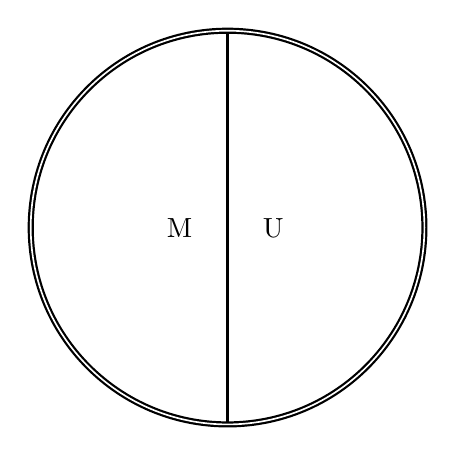
\begin{tikzpicture}[scale=.5]
			\draw[thick,double] (0,0) circle (5);
			\draw[thick] (0,-4.95) -- (0,4.95);
				\node[label={[label distance=2mm]180:M}] at (0,0) {};
				\node[label={[label distance=2mm]360:U}] at (0,0) {};
		\end{tikzpicture}}
\end{figure}